\documentclass[10pt,a4paper]{amsart}
\usepackage{amsmath,amssymb,amsthm,graphicx}
\usepackage{amsmath,amssymb,graphicx,xcolor,mathtools,listings}
\usepackage{fontspec}
\newfontfamily\proofcodefont{DejaVu Sans}
\lstset{basicstyle=\proofcodefont\tiny,breaklines=true,columns=fullflexible,keepspaces=true}
\title{Many-one reduction from simple semi-Thue zero-to-one reachability to higher-order beta-matching}
\author{Andrej Dudenhefner}
\date{doi:10.4230/LIPIcs.FSCD.2025.17; CC BY4.0 (paper); MPL2.0 (author formal library)}
\begin{document}
\maketitle
\noindent\textit{Editorial note.} Paper https://drops.dagstuhl.de/entities/document/10.4230/LIPIcs.FSCD.2025.17, CC BY4.0. Formal author code is separately MPL2.0, from snapshot70dfc56f33a6e4835281044e68aa68279989047e explicitly linked by the paper; original license is attached.\par\medskip
\noindent\textit{Editorial note.} Counted statement is Theorem39 many-one reduction. Theorem40 is its undecidability consequence and is not an additional item.\par\medskip
\noindent\textit{Allowed standard prerequisites (editorial).}\begin{itemize}
\item Simply typed lambda-calculus normalization, substitution and standard undecidability of the simple semi-Thue zero-to-one problem. Author §2, Theorem17 and referenced Coq-library foundations at fixed snapshot; core reduction code and directly linked term/type support included.
\end{itemize}\medskip
% BEGIN S2
 
\par\medskip\noindent\textbf{2 Preliminaries}\par
 
% BEGIN S2.p1
 
In this section we fix preliminaries and basic notation, following standard literature [2].\par
 
% END S2.p1
 
% BEGIN S2.SS0.SSS0.Px1
 
\par\medskip\noindent\textbf{Higher-order $\beta$-Matching in the Simply Typed $\lambda$-Calculus}\par
 
% BEGIN S2.SS0.SSS0.Px1.p1
 
The syntax of untyped $\lambda$-terms is given in the following Definition 1.\par
 
% END S2.SS0.SSS0.Px1.p1
 
% BEGIN Thmtheorem1
 
\par\medskip\noindent\textbf{Definition 1 ($\lambda$-Terms).}\par
 
% BEGIN Thmtheorem1.p1
 
$M,N::=x\mid M\,N\mid\lambda x.M$ where $a,\ldots,z$ range over term variables.\par
 
% END Thmtheorem1.p1
 
% END Thmtheorem1
 
% BEGIN S2.SS0.SSS0.Px1.p2
 
Substitution of the term variable $x$ in the term $M$ by the term $N$ is denoted $M[x:=N]$.As usual, term application associates to the left, and we may group consecutive $\lambda$-abstractions. We commonly refer to the term $\lambda x.x$ as $I$.\par
 
% END S2.SS0.SSS0.Px1.p2
 
% BEGIN Thmtheorem2
 
\par\medskip\noindent\textbf{Definition 2 ($\beta$-Reduction).}\par
 
% BEGIN Thmtheorem2.p1
 
The relation $\to_{\beta}$ on terms is the contextual closure of $(\lambda x.M)\,N\to_{\beta}M[x:=N]$.\par
 
% END Thmtheorem2.p1
 
% END Thmtheorem2
 
% BEGIN S2.SS0.SSS0.Px1.p3
 
The $\beta$-equivalence relation $=_{\beta}$ is the reflexive, transitive, symmetric closure of $\to_{\beta}$.\par
 
% END S2.SS0.SSS0.Px1.p3
 
% BEGIN S2.SS0.SSS0.Px1.p4
 
In the simply typed $\lambda$-calculus we may assign to a term $M$ a simple type $\tau$ in type environment $\Gamma$, written $\Gamma\vdash M:\tau$. Similarly to prior work [13], one ground atom $\iota$ in the construction of simple types suffices for the negative result in the present work. Definition 5 contains the rules (Var), ($\to$I), and ($\to$E) of the simple type system.\par
 
% END S2.SS0.SSS0.Px1.p4
  
% BEGIN Thmtheorem3
 
\par\medskip\noindent\textbf{Definition 3 (Simple Types with Ground Atom $\iota$).}\par
 
% BEGIN Thmtheorem3.p1
 
\par
    \[\sigma,\tau::=\iota\mid\sigma\to\tau\]    
% END Thmtheorem3.p1
 
% END Thmtheorem3
 
% BEGIN S2.SS0.SSS0.Px1.p5
 
The arrow type constructor $\to$ associates to the right.\par
 
% END S2.SS0.SSS0.Px1.p5
 
% BEGIN Thmtheorem4
 
\par\medskip\noindent\textbf{Definition 4 (Type Environments).}\par
 
% BEGIN Thmtheorem4.p1
    \[\Gamma::=\{x_{1}:\sigma_{1},\ldots,x_{n}:\sigma_{n}\}\text{ where }x_{i}\neq x%
_{j}\text{ for }i\neq j\]    
% END Thmtheorem4.p1
 
% END Thmtheorem4
 
% BEGIN Thmtheorem5
 
\par\medskip\noindent\textbf{Definition 5 (Simple Type System).}\par
 
% BEGIN Thmtheorem5.p1
 
\begin{center}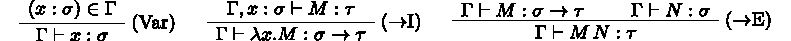
\includegraphics[width=0.95\linewidth,height=0.45\textheight,keepaspectratio]{formula-01.pdf}\end{center}\par
 
% END Thmtheorem5.p1
 
% END Thmtheorem5
 
% BEGIN S2.SS0.SSS0.Px1.p6
 
The following Example 6 illustrates a type derivation in the simple type system.\par
 
% END S2.SS0.SSS0.Px1.p6
 
% BEGIN Thmtheorem6
 
\par\medskip\noindent\textbf{Example 6.}\par
 
% BEGIN Thmtheorem6.p1
 
\begin{center}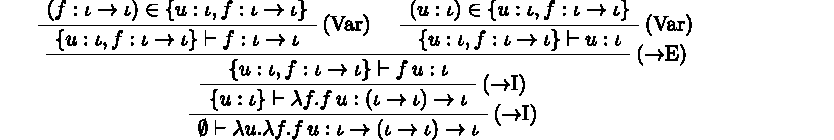
\includegraphics[width=0.95\linewidth,height=0.45\textheight,keepaspectratio]{formula-02.pdf}\end{center}
 
% END Thmtheorem6.p1
 
% END Thmtheorem6
 
% BEGIN S2.SS0.SSS0.Px1.p7
 
Higher-order $\beta$-matching is the following typed unification problem, for which only one side is subject to instantiation.\par
 
% END S2.SS0.SSS0.Px1.p7
 
% BEGIN Thmtheorem7
 
\par\medskip\noindent\textbf{Problem 7 (Higher-order $\beta$-Matching (${F}\,\mathsf{X}=N$)).}\par
 
% BEGIN Thmtheorem7.p1
 
Given terms $F,N$ and simple types $\sigma,\tau$ such that $\emptyset\vdash F:\sigma\to\tau$ and $\emptyset\vdash N:\tau$, is there a term $M$ such that $\emptyset\vdash M:\sigma$ and $F\,M=_{\beta}N$?\par
 
% END Thmtheorem7.p1
 
% END Thmtheorem7
 
% BEGIN S2.SS0.SSS0.Px1.p8
 
Undecidability of higher-order $\beta$-matching is shown by Loader [13] using a reduction from a variant of $\lambda$-definability.\par
 
% END S2.SS0.SSS0.Px1.p8
 
% BEGIN Thmtheorem8
 
\par\medskip\noindent\textbf{Theorem 8 ([13, Theorem 5.5]).}\par
 
% BEGIN Thmtheorem8.p1
 
Higher-order $\beta$-matching is undecidable.\par
 
% END Thmtheorem8.p1
 
% END Thmtheorem8
 
% BEGIN S2.SS0.SSS0.Px1.p9
 
For the remainder of the present work we use the term matching in order to refer to higher-order $\beta$-matching. Since simply typed terms are strongly normalizing and $\beta$-reduction is confluent [2], the it suffices in Problem 7 to consider terms $F,M,N$ in normal form.\par
 
% END S2.SS0.SSS0.Px1.p9
 
% BEGIN S2.SS0.SSS0.Px1.p10
 
Let us get familiar with matching by means of several illustrating examples. The following Example 9 illustrates a positive matching instance.\par
 
% END S2.SS0.SSS0.Px1.p10
 
% BEGIN Thmtheorem9
 
\par\medskip\noindent\textbf{Example 9.}\par
 
% BEGIN Thmtheorem9.p1
 
Consider the terms $F:=\lambda x.\lambda y.x\,y\,I$ and $N:=I$, for which we have $\emptyset\vdash F:(\iota\to(\iota\to\iota)\to\iota)\to(\iota\to\iota)$ and $\emptyset\vdash N:\iota\to\iota$.\par
 
% END Thmtheorem9.p1
 
% BEGIN Thmtheorem9.p2
 
The matching instance ${F}\,\mathsf{X}=N$ is solvable, including the solution $M:=\lambda u.\lambda f.f\,u$.To be precise, we have the following two properties:\par
  
\par\noindent  $\blacksquare$ 
% BEGIN S2.I1.i1.p1
 
$\emptyset\vdash M:\iota\to(\iota\to\iota)\to\iota$ (Example 6)\par
 
% END S2.I1.i1.p1
 
 
\par\noindent  $\blacksquare$ 
% BEGIN S2.I1.i2.p1
 
$F\,M=_{\beta}\lambda y.(\lambda u.\lambda f.f\,u)\,y\,I=_{\beta}\lambda y.I\,y%
=_{\beta}N$\par
 
% END S2.I1.i2.p1
 
  
% END Thmtheorem9.p2
 
% END Thmtheorem9
 
% BEGIN S2.SS0.SSS0.Px1.p11
 
We want to encode certain functional behavior as a matching instance. The following Example 10 shows a naive approach to such an encoding and its limitations.\par
 
% END S2.SS0.SSS0.Px1.p11
 
% BEGIN Thmtheorem10
 
\par\medskip\noindent\textbf{Example 10.}\par
 
% BEGIN Thmtheorem10.p1
 
Let us associate elements of the set $\{1,2,3\}$ with projections $\pi_{1}:=\lambda xyz.x$, $\pi_{2}:=\lambda xyz.y$, and $\pi_{3}:=\lambda xyz.z$ respectively. For the term $G:=\lambda h.\lambda xyz.h\,y\,z\,x$ we have $G\,\pi_{1}=_{\beta}\pi_{2}$, $G\,\pi_{2}=_{\beta}\pi_{3}$, and $G\,\pi_{3}=_{\beta}\pi_{1}$. Therefore, $G$ realizes a finite function $f_{G}:\{1,2,3\}\to\{1,2,3\}$ such that $f_{G}(1)=2$, $f_{G}(2)=3$, and $f_{G}(3)=1$.\par
 
% END Thmtheorem10.p1
 
% BEGIN Thmtheorem10.p2
 
Let $\kappa:=\iota\to\iota\to\iota\to\iota$ be a simple type for which we have $\emptyset\vdash\pi_{i}:\kappa$ for $i\in\{1,2,3\}$. Consider the matching instance $F\,\mathsf{X}=\pi_{3}$, where $F:=\lambda t.t\,G\,\pi_{1}$, and for which we have $\emptyset\vdash F:((\kappa\to\kappa)\to\kappa\to\kappa)\to\kappa$. The intended “meaning” of this matching instance is: starting with the element $1$, repeatedly apply the function $f_{G}$ in order to construct the element $3$.\par
 
% END Thmtheorem10.p2
 
% BEGIN Thmtheorem10.p3
 
One solution for this instance is the term $\lambda f.\lambda s.f\,(f\,s)$ for which we have:\par
    \[F\,(\lambda f.\lambda s.f\,(f\,s))=_{\beta}f\,(f\,s)[f:=G,s:=\pi_{1}]=_{\beta}%
G\,\pi_{2}=_{\beta}\pi_{3}\]    
This solution follows the intended meaning of the underlying representation, constructing the element $f_{G}(f_{G}(1))=3$. Another solution is $\lambda f.\lambda s.f\,(f\,(f\,(f\,(f\,s))))$, which utilizes $f_{G}(f_{G}(f_{G}(f_{G}(f_{G}(1)))))=3$.\par
 
% END Thmtheorem10.p3
 
% BEGIN Thmtheorem10.p4
 
Unfortunately, there are solutions to the above matching instance which behave differently. One such solution is $\lambda f.\lambda s.\pi_{3}$, for which we also have $F\,(\lambda f.\lambda s.\pi_{3})=_{\beta}\pi_{3}$. In this case, the element $3$ is constructed “ad hoc”, with no reference to the provided arguments. Another solution is the term $\lambda f.\lambda s.\lambda xyz.f\,s\,z\,z\,z$. This solution exploits the exact representation of elements via projections, disregarding any intended meaning of the underlying representation.\par
 
% END Thmtheorem10.p4
 
% END Thmtheorem10
 
% BEGIN S2.SS0.SSS0.Px1.p12
 
In the above Example 10 we would like to exclude certain ad hoc solutions, in order to faithfully encode intended functional behavior. Towards this aim, a known technique how to restrict the shape of solutions is illustrated in the following Example 11.\par
 
% END S2.SS0.SSS0.Px1.p12
 
% BEGIN Thmtheorem11
 
\par\medskip\noindent\textbf{Example 11 ([5, Proposition 3.4]).}\par
 
% BEGIN Thmtheorem11.p1
 
Consider a term $M$ in normal form such that $M\,I\,u=_{\beta}u$ where $u$ is a term variable, and $\emptyset\vdash M:(\kappa\to\kappa)\to\kappa\to\kappa$. By case analysis on $M$ we have that $M=\lambda f.\lambda s.N$ for some term $N$ in normal form. Furthermore, $\{f:\kappa\to\kappa,s:\kappa\}\vdash N:\kappa$ and $N[f:=\lambda x.x,s:=u]=_{\beta}u$. Therefore, the term $N$ is not an abstraction. By induction on the size of $N$ and case analysis of the normal form we have that $N=s$ or $N=f\,(\ldots(f\,s)\ldots)$. Since the term $M$ contains exactly two $\lambda$-abstractions, it cannot be an ad hoc solution from Example 10.\par
 
% END Thmtheorem11.p1
 
% END Thmtheorem11
 
% BEGIN S2.SS0.SSS0.Px1.p13
 
Combining Example 10 with Example 11, we formulate in the following Example 12 a matching instance which faithfully encodes the desired functional behavior.\par
 
% END S2.SS0.SSS0.Px1.p13
 
% BEGIN Thmtheorem12
 
\par\medskip\noindent\textbf{Example 12.}\par
 
% BEGIN Thmtheorem12.p1
 
Let $F:=\lambda t.\lambda r.r\,(t\,G\,\pi_{1})\,(\lambda u.t\,I\,u)$ and $N:=\lambda r.r\,\pi_{3}\,(\lambda u.u)$ where the term $G=\lambda h.\lambda xyz.h\,y\,z\,x$ is from Example 10. We have\par
  
\par\noindent  $\blacksquare$ 
% BEGIN S2.I2.i1.p1
 
$\emptyset\vdash F:((\kappa\to\kappa)\to\kappa\to\kappa)\to(\kappa\to(\kappa\to%
\kappa)\to\iota)\to\iota$\par
 
% END S2.I2.i1.p1
 
 
\par\noindent  $\blacksquare$ 
% BEGIN S2.I2.i2.p1
 
$\emptyset\vdash N:(\kappa\to(\kappa\to\kappa)\to\iota)\to\iota$\par
 
% END S2.I2.i2.p1
 
  
The matching instance $F\,\mathsf{X}=N$ combines the matching instance from Example 10 with the additional restriction from Example 11. Therefore, solutions such as $\lambda f.\lambda s.f\,(f\,s)$ and $\lambda f.\lambda s.f\,(f\,(f\,(f\,(f\,s))))$ from Example 10 which follow the intended “meaning” of the underlying representation still solve $F\,\mathsf{X}=N$. However, ad hoc solutions such as $\lambda f.\lambda s.\pi_{3}$ or $\lambda f.\lambda s.\lambda xyz.f\,s\,z\,z\,z$ from Example 10 do not solve $F\,\mathsf{X}=N$ because such solutions contain too many $\lambda$-abstractions.\par
 
% END Thmtheorem12.p1
 
% END Thmtheorem12
 
% BEGIN Thmtheorem13
 
\par\medskip\noindent\textbf{$\blacktriangleright$ Remark 13.}\par
 
% BEGIN Thmtheorem13.p1
 
Without the restriction $\emptyset\vdash M:(\kappa\to\kappa)\to\kappa\to\kappa$ in Example 11 the term $M:=\lambda f.\lambda s.f\,f\,s$ satisfies $M\,I\,u=_{\beta}u$. However, Example 12 does not admit $M$ as a solution. The present work relies on well-typedness, but might be adapted to an untyped scenario.\par
 
% END Thmtheorem13.p1
 
% END Thmtheorem13
 
% BEGIN S2.SS0.SSS0.Px1.p14
 
The following Remark 14 illustrates how the addition of $\eta$-reduction would make the technique from Example 12 (as well as Loader’s approach) unsuitable.\par
 
% END S2.SS0.SSS0.Px1.p14
 
% BEGIN Thmtheorem14
 
\par\medskip\noindent\textbf{$\blacktriangleright$ Remark 14.}\par
 
% BEGIN Thmtheorem14.p1
 
Example 11 demonstrates how to restrict the number of abstractions in solutions. However, in the presence of $\eta$-reduction (contextual closure of $\lambda x.f\,x\to_{\eta}f$) this does not work, as shown below. Consider the terms $G:=\lambda h.\lambda xyz.h\,y\,z\,x$, $\pi_{1}=\lambda xyz.x$, $\pi_{2}=\lambda xyz.y$, and $\pi_{3}=\lambda xyz.z$ from Example 11. The term $M:=\lambda g.\lambda h.\lambda xyz.h\,(g\,\pi_{1}x\,z\,y)\,y\,z$ solves the matching instance in Example 12 because:\par
    \[\begin{array}[t]{lclcl}M\,G\,\pi_{1}&=_{\beta}&\big{(}\lambda g.\lambda h.%
\lambda xyz.h\,(g\,\pi_{1}x\,z\,y)\,y\,z\big{)}\,G\,\pi_{1}&=_{\beta}&\lambda
xyz%
.\pi_{1}\,(G\,\pi_{1}x\,z\,y)\,y\,z\\
&=_{\beta}&\lambda xyz.G\,\pi_{1}x\,z\,y&=_{\beta}&\lambda xyz.\pi_{1}\,z\,y\,%
x=_{\beta}\lambda xyz.z=\pi_{3}\end{array}\]       \[\begin{array}[t]{lclcl}M\,I\,u&=_{\beta}&\big{(}\lambda g.\lambda h.\lambda xyz%
.h\,(g\,\pi_{1}x\,z\,y)\,y\,z\big{)}\,I\,u&=_{\beta}&\lambda xyz.u\,(I\,\pi_{1%
}x\,z\,y)\,y\,z\\
&=_{\beta}&\lambda xyz.u\,(\pi_{1}x\,z\,y)\,y\,z&=_{\beta}&\lambda xyz.u\,x\,y%
\,z\to_{\eta}^{*}u\end{array}\]    
In particular, $\eta$-reduction allows for additional $\lambda$-abstractions in the solution, making the technique from Example 11 unsuitable.\par
 
% END Thmtheorem14.p1
 
% END Thmtheorem14
 
% BEGIN S2.SS0.SSS0.Px1.p15
 
The observation from Example 12 is generalized by Loader to encode arbitrary families of finite functions. This results in undecidability of higher-order $\beta$-matching by reduction from a variant of $\lambda$-definability. Loader’s generalization is quite sophisticated, as it requires construction principles to restrict shapes of realizers of arbitrary higher-order finite functions. In the present work, we focus on a fragment which can be identified by inspection of intersection types occurring in the undecidability proof of intersection type inhabitation [20, 6] and their relationship to finite model theory [15]. This leads to a simpler undecidability proof and reveals a connection between matching, intersection type inhabitation, and $\lambda$-definability. The presented approach has similarities with Joly’s [11] refinement of Loader’s proof. Joly shifts the technical burden to a particular $\lambda$-definability problem, which then is simpler to handle. Instead, we avoid $\lambda$-definability altogether and use a rewriting problem in a restricted class of simple semi-Thue systems as a starting point.\par
 
% END S2.SS0.SSS0.Px1.p15
 
% END S2.SS0.SSS0.Px1
 
% BEGIN S2.SS0.SSS0.Px2
 
\par\medskip\noindent\textbf{Simple Semi-Thue Systems}\par
 
% BEGIN S2.SS0.SSS0.Px2.p1
 
A simple semi-Thue system (Definition 15) is a rewriting system of restricted shape, introduced by Urzyczyn [20] in order to show undecidability of intersection type inhabitation.\par
 
% END S2.SS0.SSS0.Px2.p1
 
% BEGIN Thmtheorem15
 
\par\medskip\noindent\textbf{Definition 15 (Simple Semi-Thue System).}\par
 
% BEGIN Thmtheorem15.p1
 
A semi-Thue system $\mathfrak{R}$ over an alphabet $\mathcal{A}$ is simple, if each rule has the shape $ab\Rightarrow cd$ for $a,b,c,d\in\mathcal{A}$.\par
 
% END Thmtheorem15.p1
 
% END Thmtheorem15
 
% BEGIN S2.SS0.SSS0.Px2.p2
 
The reflexive, transitive closure of the rewriting relation for a given simple semi-Thue system $\mathfrak{R}$ is denoted $\Rightarrow_{\mathfrak{R}}^{*}$. For arbitrary simple semi-Thue systems it is undecidable whether some non-empty sequence of $\mathbf{0}$s can be transformed into a non-empty sequence of $\mathbf{1}$s.\par
 
% END S2.SS0.SSS0.Px2.p2
 
% BEGIN Thmtheorem16
 
\par\medskip\noindent\textbf{Problem 16 ($\mathbf{0}^{+}\Rightarrow^{*}\mathbf{1}^{+}$).}\par
 
% BEGIN Thmtheorem16.p1
 
Given a simple semi-Thue system $\mathfrak{R}$, does $\mathbf{0}^{n}\Rightarrow^{*}_{\mathfrak{R}}\mathbf{1}^{n}$ hold for some $n>0$?\par
 
% END Thmtheorem16.p1
 
% END Thmtheorem16
 
% BEGIN Thmtheorem17
 
\par\medskip\noindent\textbf{Theorem 17 ([6, Lemma 3.3]).}\par
 
% BEGIN Thmtheorem17.p1
 
Problem $\mathbf{0}^{+}\Rightarrow^{*}\mathbf{1}^{+}$ is undecidable.\par
 
% END Thmtheorem17.p1
 
% END Thmtheorem17
 
% BEGIN S2.SS0.SSS0.Px2.p3
 
The following Example 18 illustrates a positive instance of Problem $\mathbf{0}^{+}\Rightarrow^{*}\mathbf{1}^{+}$.\par
 
% END S2.SS0.SSS0.Px2.p3
 
% BEGIN Thmtheorem18
 
\par\medskip\noindent\textbf{Example 18.}\par
 
% BEGIN Thmtheorem18.p1
 
Let $\mathfrak{R}:=\{\mathbf{0}\mathbf{0}\Rightarrow\mathbf{2}\mathbf{2},\mathbf{0}%
\mathbf{2}\Rightarrow\mathbf{1}\mathbf{1},\mathbf{2}\mathbf{0}\Rightarrow%
\mathbf{1}\mathbf{1}\}$ be a simple semi-Thue system over the alphabet $\{\mathbf{0},\mathbf{1},\mathbf{2}\}$. We have $\mathbf{0}\mathbf{0}\mathbf{0}\mathbf{0}\Rightarrow_{\mathfrak{R}}\mathbf{0}%
\mathbf{2}\mathbf{2}\mathbf{0}\Rightarrow_{\mathfrak{R}}\mathbf{1}\mathbf{1}%
\mathbf{2}\mathbf{0}\Rightarrow_{\mathfrak{R}}\mathbf{1}\mathbf{1}\mathbf{1}%
\mathbf{1}$. As a side note, we have $\mathbf{0}^{n}\;{\not\Rightarrow}_{\mathfrak{R}}^{*}\;\mathbf{1}^{n}$ for $n\in\{1,2,3\}$.\par
 
% END Thmtheorem18.p1
 
% END Thmtheorem18
 
% BEGIN Thmtheorem19
 
\par\medskip\noindent\textbf{$\blacktriangleright$ Remark 19.}\par
 
% BEGIN Thmtheorem19.p1
 
Problem $\mathbf{0}^{+}\Rightarrow^{*}\mathbf{1}^{+}$ is used as a starting point in a refinement [6, Lemma 4.4] of Urzyczyn’s undecidability result for intersection type inhabitation [20]. Undecidability of Problem $\mathbf{0}^{+}\Rightarrow^{*}\mathbf{1}^{+}$ is mechanized as part of Coq Library of Undecidability Proofs [8], making it a good starting point for further mechanized undecidability results.\par
 
% END Thmtheorem19.p1
 
% END Thmtheorem19
 
% END S2.SS0.SSS0.Px2
 
% END S2

% BEGIN S4
 
\par\medskip\noindent\textbf{4 Mechanization}\par
 
% BEGIN S4.p1
 
This section provides a brief overview over the mechanization of undecidability of higher-order $\beta$-matching (Theorem 40) using the Coq proof assistant [19]. The mechanization is constructive (in the technical sense of axiom-free Coq) and spans approximately $4000$ lines of code, consisting of the following parts:\par
  
\par\noindent  $\blacksquare$ 
% BEGIN S4.I1.i1.p1
 
HOMatching.v contains definitions of the simply typed $\lambda$-calculus [ ] and higher-order $\beta$-matching [ ].\par
 
% END S4.I1.i1.p1
 
 
\par\noindent  $\blacksquare$ 
% BEGIN S4.I1.i2.p1
 
Util/stlc\_facts.v and Util/term\_facts.v contain basic properties of the simply typed $\lambda$-calculus, such as confluence of $\beta$-reduction [ ], substitution lemmas [ ], and type preservation properties [ ].\par
 
% END S4.I1.i2.p1
 
 
\par\noindent  $\blacksquare$ 
% BEGIN S4.I1.i3.p1
 
Reductions/SSTS01\_to\_HOMbeta.v contains the reduction from Problem $\mathbf{0}^{+}\Rightarrow^{*}\mathbf{1}^{+}$ to higher-order $\beta$-matching [ ].\par
 
% END S4.I1.i3.p1
 
 
\par\noindent  $\blacksquare$ 
% BEGIN S4.I1.i4.p1
 
HOMatching\_undec.v contains the undecidability result for higher-order $\beta$-matching [ ].\par
 
% END S4.I1.i4.p1
 
  
% END S4.p1
 
% BEGIN S4.p2
 
The simple type system stlc is mechanized in HOMatching.v, borrowing the existing term definitions from the library [ ], for which variable binding is addressed via the unscoped de Bruijn approach [4]. The proposition stlc Gamma M t mechanizes that the term M is assigned the simple type t in the simple type environment Gamma.\par
  \ensuremath{\downarrow} 
% BEGIN lstnumberx1
 Inductive ty : Type := 
% END lstnumberx1
 
% BEGIN lstnumberx2
  | atom (* type variable *) 
% END lstnumberx2
 
% BEGIN lstnumberx3
  | arr (s t : ty). (* function type *) 
% END lstnumberx3
 
% BEGIN lstnumberx4
 
% END lstnumberx4
 
% BEGIN lstnumberx5
 Inductive term : Type := 
% END lstnumberx5
 
% BEGIN lstnumberx6
  | var (n : nat) : term (* term variable *) 
% END lstnumberx6
 
% BEGIN lstnumberx7
  | app (s : term) (t : term) : term (* application *) 
% END lstnumberx7
 
% BEGIN lstnumberx8
  | lam (s : term). (* abstraction *) 
% END lstnumberx8
 
% BEGIN lstnumberx9
 
% END lstnumberx9
 
% BEGIN lstnumberx10
 Inductive stlc (Gamma : list ty) : term -> ty -> Prop := 
% END lstnumberx10
 
% BEGIN lstnumberx11
  | stlc\_var x t : nth\_error Gamma x = Some t -> 
% END lstnumberx11
 
% BEGIN lstnumberx12
  stlc Gamma (var x) t (* variable rule *) 
% END lstnumberx12
 
% BEGIN lstnumberx13
  | stlc\_app M N s t : stlc Gamma M (arr s t) -> stlc Gamma N s -> 
% END lstnumberx13
 
% BEGIN lstnumberx14
  stlc Gamma (app M N) t (* application rule *) 
% END lstnumberx14
 
% BEGIN lstnumberx15
  | stlc\_lam M s t : stlc (cons s Gamma) M t -> 
% END lstnumberx15
 
% BEGIN lstnumberx16
  stlc Gamma (lam M) (arr s t). (* abstraction rule *) 
% END lstnumberx16
  
% END S4.p2
 
% BEGIN S4.p3
 
Higher-order $\beta$-matching is mechanized as the predicate HOMbeta: given terms F of type arr s t and N of type t, is there a simply typed term M of type s such that app F M is $\beta$-equivalent (reflexive, symmetric, transitive closure of step) to N?\par
  \ensuremath{\downarrow} 
% BEGIN lstnumberx17
 Definition HOMbeta : \{ ’(s, t, F, N) : (ty * ty * term * term) 
% END lstnumberx17
 
% BEGIN lstnumberx18
  | stlc nil F (arr s t) /\textbackslash{} stlc nil N t \} -> Prop := 
% END lstnumberx18
 
% BEGIN lstnumberx19
  fun ’(exist \_ (s, t, F, N) \_) => 
% END lstnumberx19
 
% BEGIN lstnumberx20
  exists (M : term), stlc nil M s /\textbackslash{} 
% END lstnumberx20
 
% BEGIN lstnumberx21
  clos\_refl\_sym\_trans term step (app F M) N. 
% END lstnumberx21
  
% END S4.p3
 
% BEGIN S4.p4
 
The proposition undecidable HOMbeta [ ] mechanizes the undecidability of the predicate HOMbeta, relying on the following library definition [7, Chapter 19]. A predicate p is undecidable, if existence of a computable decider for p implies recursive co-enumerability of the (Turing machine) Halting Problem.\par
  \ensuremath{\downarrow} 
% BEGIN lstnumberx22
 Definition undecidable \{X\} (p : X -> Prop) := 
% END lstnumberx22
 
% BEGIN lstnumberx23
  decidable p -> enumerable (complement SBTM\_HALT). 
% END lstnumberx23
  
Since the Halting Problem is recursively enumerable, decidability of p would imply decidability of the Halting Problem.\par
 
% END S4.p4
 
% END S4

% BEGIN Thmtheorem39
 
\par\medskip\noindent\textbf{Theorem 39.}\par
 
% BEGIN Thmtheorem39.p1
 
Problem $\mathbf{0}^{+}\Rightarrow^{*}\mathbf{1}^{+}$ many-one reduces to higher-order $\beta$-matching.\par
 
% END Thmtheorem39.p1
 
% END Thmtheorem39

% BEGIN S3
 
\par\medskip\noindent\textbf{3 Undecidability of Higher-order $\beta$-Matching}\par
 
% BEGIN S3.p1
 
In this section we develop our main result (Theorem 39): a reduction from the rewriting problem $\mathbf{0}^{+}\Rightarrow^{*}\mathbf{1}^{+}$ to higher-order $\beta$-matching.\par
 
% END S3.p1
 
% BEGIN S3.p2
 
For the remainder of the section we fix the simple semi-Thue system $\mathfrak{R}:=\{R_{1},\ldots,R_{L}\}$ with $L>0$ rules over the finite alphabet $\{\mathbf{0},\mathbf{1},\mathbf{2},\ldots,\mathbf{K}\}$. Our approach is to construct simply typed terms which capture the two main aspects of the rewriting problem $\mathbf{0}^{+}\Rightarrow^{*}\mathbf{1}^{+}$: the search for a sufficiently long starting sequence of $\mathbf{0}$s, and the individual rewriting steps to the desired sequence of $\mathbf{1}$s.\par
 
% END S3.p2
 
% BEGIN S3.p3
 
The remainder of the present section is structured as follows. First, we fix basic notation, encoding, and properties of the rewriting in the system $\mathfrak{R}$. Second, we restrict the shape of potential solutions for the constructed matching instance, similarly to Example 11. Third, for solutions of restricted shape we capture the functional properties of the rewriting problem $\mathbf{0}^{+}\Rightarrow^{*}\mathbf{1}^{+}$.\par
 
% END S3.p3
 
% BEGIN S3.SSx1
 
\par\medskip\noindent\textbf{Notation}\par
 
% BEGIN S3.SSx1.p1
 
We introduce four additional symbols in extended alphabet $\mathcal{A}:=\{\mathbf{0},\mathbf{1},\ldots,\mathbf{K}\}\cup\{\$,\bullet,\top,\bot\}$. We represent an alphabet symbol $i\in\mathcal{A}$ as the projection $\pi_{i}:=\lambda s_{\mathbf{0}}s_{\mathbf{1}}\ldots s_{\mathbf{K}}s_{\$}s_{%
\bullet}s_{\top}s_{\bot}.s_{i}$ typed by the simple type $\kappa:=\underbracket{\iota\to\ldots\to\iota}_{|\mathcal{A}|\leavevmode%
\nobreak\ \text{times}}\to\iota$. The intended meaning of the additional symbols in the extended alphabet is as follows. The symbol $\$$ marks the beginning of a word for word expansion, $\bullet$ serves as symbol different from $\mathbf{0}$ and $\mathbf{1}$ for case analysis, $\top$ serves as a constructible symbol, and $\bot$ serves as a non-constructible symbol.\par
 
% END S3.SSx1.p1
 
% BEGIN S3.SSx1.p2
 
For readability, we use the following case notation to match individual symbols.\par
 
% END S3.SSx1.p2
 
% BEGIN Thmtheorem20
 
\par\medskip\noindent\textbf{Definition 20 (case).}\par
 
% BEGIN Thmtheorem20.p1
 
For $k\in\mathbb{N}$, distinct $i_{1},\ldots,i_{k}\in\mathcal{A}$, and terms $M_{1},\ldots,M_{k}$:\par
    $\displaystyle\textnormal{{case }}{x}\textnormal{{ of }}\langle M\mid i_{1}%
\mapsto M_{1}\mid\ldots\mid i_{k}\mapsto M_{k}\rangle:=$ $\displaystyle\leavevmode\nobreak\ x\,N_{\mathbf{0}}\,N_{\mathbf{1}}\ldots N_{%
\mathbf{K}}\,N_{\$}\,N_{\bullet}\,N_{\top}\,N_{\bot}$      $\displaystyle\text{ where }N_{i}=\begin{cases}M_{j}&\text{if }i=i_{j}\\
M&\text{otherwise}\end{cases}$    
% END Thmtheorem20.p1
 
% END Thmtheorem20
 
% BEGIN S3.SSx1.p3
 
A particular term $\delta_{i}$ for $i\in\mathcal{A}$, which we use commonly is:\par
    \[\delta_{i}:=\lambda x.\lambda s_{\mathbf{0}}s_{\mathbf{1}}\ldots s_{\mathbf{K}%
}s_{\$}s_{\bullet}s_{\top}s_{\bot}.\textnormal{{case }}{x}\textnormal{{ of }}%
\langle s_{\bot}\mid\top\mapsto s_{i}\rangle\]    
We have $\emptyset\vdash\delta_{i}:\kappa\to\kappa$, and the following Lemma 21 specifies the behavior of $\delta_{i}$.\par
 
% END S3.SSx1.p3
 
% BEGIN Thmtheorem21
 
\par\medskip\noindent\textbf{Lemma 21.}\par
 
% BEGIN Thmtheorem21.p1
 
For $i,j\in\mathcal{A}$ such that $i\neq j$ we have $\delta_{i}\,\pi_{\top}=_{\beta}\pi_{i}$ and $\delta_{i}\,\pi_{j}=_{\beta}\pi_{\bot}$.\par
 
% END Thmtheorem21.p1
 
% END Thmtheorem21
 
% END S3.SSx1
 
% BEGIN S3.SSx2
 
\par\medskip\noindent\textbf{Syntactic Constraints}\par
 
% BEGIN S3.SSx2.p1
 
We identify the shape of “well-formed” terms, suitable to represent rewriting. In the following Definition 22 terms in the set $\mathcal{Q}_{m}$ capture consecutive rule application for a word of length $m+1$, ending in the word $\mathbf{1}^{m+1}$ (represented by $z_{\mathbf{1}}\in\mathcal{Q}_{m}$). The subterm $r_{i}\,p_{j}$ (and $r_{i}\,(\lambda w.p_{j}\,w)$) for $i\in\{1,\ldots,L\}$ and $j\in\{1,\ldots,m\}$ indicates an application of the rule $R_{i}$ at position $j$. Additionally, terms in the set $\mathcal{R}_{m}$ capture consecutive increase of word length starting with $m+1$, and initialization with $\mathbf{0}$s before rewriting (represented by $z_{\mathbf{0}}\,N\,M\in\mathcal{R}_{m}$ for $M\in\mathcal{Q}_{m}$). Specifically, the subterm $z_{\star}\,N\,(\lambda p_{m+1}.M)$ introduces an additional bound variable $p_{m+1}$ in order to argue about rule application at position $m+1$ in the longer word. Consequently, terms in $\mathcal{R}_{1}$ represent witnesses for an arbitrary expansion of a word starting with length $2$, followed by initialization with $\mathbf{0}$s, and consecutive rule application (potentially ending in $\mathbf{1}$s).\par
 
% END S3.SSx2.p1
 
% BEGIN Thmtheorem22
 
\par\medskip\noindent\textbf{Definition 22 (Sets $\mathcal{Q}_{m}$, $\mathcal{R}_{m}$ of Terms).}\par
 
% BEGIN Thmtheorem22.p1
 
For $m>0$, let $\mathcal{Q}_{m}$ and $\mathcal{R}_{m}$ be the smallest sets of terms satisfying the following rules:\par
  
\par\noindent  $\blacksquare$ 
% BEGIN S3.I1.i1.p1
 
$z_{\mathbf{1}}\in\mathcal{Q}_{m}$\par
 
% END S3.I1.i1.p1
 
 
\par\noindent  $\blacksquare$ 
% BEGIN S3.I1.i2.p1
 
if $M\in\mathcal{Q}_{m}$ then $(r_{i}\,p_{j}\,M)\in\mathcal{Q}_{m}$ for $i\in\{1,\ldots,L\}$ and $j\in\{1,\ldots,m\}$\par
 
% END S3.I1.i2.p1
 
 
\par\noindent  $\blacksquare$ 
% BEGIN S3.I1.i3.p1
 
if $M\in\mathcal{Q}_{m}$ then $(r_{i}\,(\lambda w.p_{j}\,w)\,M)\in\mathcal{Q}_{m}$ for $i\in\{1,\ldots,L\}$ and $j\in\{1,\ldots,m\}$\par
 
% END S3.I1.i3.p1
 
 
\par\noindent  $\blacksquare$ 
% BEGIN S3.I1.i4.p1
 
if $M\in\mathcal{Q}_{m}$ then $(z_{\mathbf{0}}\,N\,M)\in\mathcal{R}_{m}$\par
 
% END S3.I1.i4.p1
 
 
\par\noindent  $\blacksquare$ 
% BEGIN S3.I1.i5.p1
 
if $M\in\mathcal{R}_{m+1}$ then $(z_{\star}\,N\,(\lambda p_{m+1}.M))\in\mathcal{R}_{m}$\par
 
% END S3.I1.i5.p1
 
  
% END Thmtheorem22.p1
 
% END Thmtheorem22
 
% BEGIN Thmtheorem23
 
\par\medskip\noindent\textbf{$\blacktriangleright$ Remark 23.}\par
 
% BEGIN Thmtheorem23.p1
 
Terms in $\mathcal{R}_{1}$ are inspired by inhabitants in a refinement [6, Lemma 4.4] of Urzyczyn’s undecidability result for intersection type inhabitation [20].\par
 
% END Thmtheorem23.p1
 
% END Thmtheorem23
 
% BEGIN S3.SSx2.p2
 
Free variables occurring in terms in $\mathcal{Q}_{m}$ and $\mathcal{R}_{m}$ are assigned simple types according to the following type environment $\Gamma_{m}$, such that terms in $\mathcal{Q}_{m}$ and $\mathcal{R}_{m}$ can be assigned the simple type $\kappa$.\par
 
% END S3.SSx2.p2
 
% BEGIN Thmtheorem24
 
\par\medskip\noindent\textbf{Definition 24 (Type Environment $\Gamma_{m}$).}\par
 
% BEGIN Thmtheorem24.p1
 
For $m>0$ let\par
    $\displaystyle\Gamma_{m}$ $\displaystyle:=\{\begin{aligned} &z_{\mathbf{1}}:\kappa,z_{\mathbf{0}}:(\kappa%
\to\kappa)\to\kappa\to\kappa,z_{\star}:(\kappa\to\kappa)\to((\kappa\to\kappa)%
\to\kappa)\to\kappa,\\
&p_{1}:\kappa\to\kappa,\ldots,p_{m}:\kappa\to\kappa,\\
&r_{1}:(\kappa\to\kappa)\to\kappa\to\kappa,\ldots,r_{L}:(\kappa\to\kappa)\to%
\kappa\to\kappa\}\end{aligned}$    
% END Thmtheorem24.p1
 
% END Thmtheorem24
 
% BEGIN S3.SSx2.p3
 
Similarly to Example 11, we formulate typed terms (Definition 25) and $\beta$-equivalence constraints characterizing members of $\mathcal{Q}_{m}$ (Lemma 27) and $\mathcal{R}_{m}$ (Lemma 28).\par
 
% END S3.SSx2.p3
 
% BEGIN Thmtheorem25
 
\par\medskip\noindent\textbf{Definition 25 (Typed Terms $H_{\star}$, $H_{\mathbf{0}}$, $H_{R}$).}\par
 
% BEGIN Thmtheorem25.p1
    $\displaystyle H_{\star}:=$ $\displaystyle\lambda h.\lambda g.\lambda s_{\mathbf{0}}s_{\mathbf{1}}\ldots s_%
{\mathbf{K}}s_{\$}s_{\bullet}s_{\top}s_{\bot}.\textnormal{{case }}{g\,\delta_{%
\bullet}}\textnormal{{ of }}\langle s_{\bot}\mid\$\mapsto s_{\$}\rangle$     $\displaystyle H_{\mathbf{0}}:=$ $\displaystyle\lambda h.\lambda x.\lambda s_{\mathbf{0}}s_{\mathbf{1}}\ldots s_%
{\mathbf{K}}s_{\$}s_{\bullet}s_{\top}s_{\bot}.\textnormal{{case }}{x}%
\textnormal{{ of }}\langle s_{\bot}\mid\mathbf{1}\mapsto s_{\$}\rangle$     $\displaystyle H_{R}:=$ $\displaystyle\lambda h.\lambda x.\lambda s_{\mathbf{0}}s_{\mathbf{1}}\ldots s_%
{\mathbf{K}}s_{\$}s_{\bullet}s_{\top}s_{\bot}.\textnormal{{case }}{h\,\pi_{%
\top}}\textnormal{{ of }}\langle s_{\bot}\mid\bullet\mapsto\textnormal{{case }%
}{x}\textnormal{{ of }}\langle s_{\bot}\mid\mathbf{1}\mapsto s_{\mathbf{1}}\rangle\rangle$       \[\emptyset\vdash H_{\star}:\Gamma_{m}(z_{\star})\qquad\quad\emptyset\vdash H_{%
\mathbf{0}}:\Gamma_{m}(z_{\mathbf{0}})\qquad\quad\emptyset\vdash H_{R}:\Gamma_%
{m}(r_{i})\text{ for }i\in\{1,\ldots,L\}\]    
% END Thmtheorem25.p1
 
% END Thmtheorem25
 
% BEGIN S3.SSx2.p4
 
We introduce substitutions $S_{F}$ and $S_{H}$ acting on the term variables $z_{\star},z_{\mathbf{1}},z_{\mathbf{0}},r_{1},\ldots,r_{L}$, which occur in terms in $\mathcal{Q}_{m}$ and $\mathcal{R}_{m}$.\par
 
% END S3.SSx2.p4
 
% BEGIN Thmtheorem26
 
\par\medskip\noindent\textbf{Definition 26 (Substitutions $S_{F}$, $S_{H}$).}\par
 
% BEGIN Thmtheorem26.p1
    \[\begin{array}[]{llll}S_{F}(z_{\star}):=\lambda h.\lambda g.g\,I\nobreak%
\leavevmode&S_{F}(z_{\mathbf{1}}):=u\nobreak\leavevmode&S_{F}(z_{\mathbf{0}}):%
=\lambda h.I\nobreak\leavevmode&S_{F}(r_{j}):=I\text{ for }j\in{1,\ldots L}\\
S_{H}(z_{\star}):=H_{\star}&S_{H}(z_{\mathbf{1}}):=\pi_{\mathbf{1}}&S_{H}(z_{%
\mathbf{0}}):=H_{\mathbf{0}}&S_{H}(r_{j}):=H_{R}\text{ for }j\in{1,\ldots L}%
\end{array}\]    
% END Thmtheorem26.p1
 
% END Thmtheorem26
 
% BEGIN Thmtheorem27
 
\par\medskip\noindent\textbf{Lemma 27.}\par
 
% BEGIN Thmtheorem27.p1
 
For $m>0$, if a term $M$ is in normal form such that $\Gamma_{m}\vdash M:\kappa$, $S_{F}(M)[p_{1}{\,:=\,}I,\ldots,p_{m}{\,:=\,}I]=_{\beta}u$, and $S_{H}(M)[p_{1}:=\delta_{\bullet},\ldots,p_{m}:=\delta_{\bullet}]=_{\beta}\pi_{%
\mathbf{1}}$, then $M\in\mathcal{Q}_{m}$.\par
 
% END Thmtheorem27.p1
 
% END Thmtheorem27
 
% BEGIN S3.SSx2.SSS0.P0.SPx1
 
\par\medskip\noindent\textbf{Proof.}\par
 
% BEGIN S3.SSx2.SSS0.P0.SPx1.p1
 
Induction on the size of $M$ and case analysis of the normal form. $\hfill\blacktriangleleft$\par
 
% END S3.SSx2.SSS0.P0.SPx1.p1
 
% BEGIN Thmtheorem28
 
\par\medskip\noindent\textbf{Lemma 28.}\par
 
% BEGIN Thmtheorem28.p1
 
For $m>0$, if a term $M$ is in normal form such that $\Gamma_{m}\vdash M:\kappa$, $S_{F}(M)[p_{1}{\,:=\,}I,\ldots,p_{m}{\,:=\,}I]=_{\beta}u$, and $S_{H}(M)[p_{1}:=\delta_{\bullet},\ldots,p_{m}:=\delta_{\bullet}]=_{\beta}\pi_{\$}$, then $M\in\mathcal{R}_{m}$.\par
 
% END Thmtheorem28.p1
 
% END Thmtheorem28
 
% END S3.SSx2.SSS0.P0.SPx1
 
% BEGIN S3.SSx2.SSS0.P0.SPx2
 
\par\medskip\noindent\textbf{Proof.}\par
 
% BEGIN S3.SSx2.SSS0.P0.SPx2.p1
 
Induction on the size of $M$, case analysis of the normal form, and Lemma 27. $\hfill\blacktriangleleft$\par
 
% END S3.SSx2.SSS0.P0.SPx2.p1
 
% BEGIN S3.SSx2.SSS0.P0.SPx2.p2
 
As a consequence of the above Lemma 28, the following Theorem 29 presents $\beta$-equivalence constraints which suffice to restrict the shape of terms under consideration.\par
 
% END S3.SSx2.SSS0.P0.SPx2.p2
 
% BEGIN Thmtheorem29
 
\par\medskip\noindent\textbf{Theorem 29.}\par
 
% BEGIN Thmtheorem29.p1
 
If a term $M$ is in normal form such that $\emptyset\vdash M:\Gamma_{1}(r_{1})\to\cdots\to\Gamma_{1}(r_{L})\to\Gamma_{1}(%
z_{\mathbf{0}})\to\Gamma_{1}(z_{\mathbf{1}})\to\Gamma_{1}(z_{\star})\to\Gamma_%
{1}(p_{1})\to\kappa$, $M\,I\ldots I\,(\lambda h.I)\,u\,(\lambda h.\lambda g.g\,I)\,I=_{\beta}u$, and $M\,H_{R}\ldots H_{R}\,H_{\mathbf{0}}\,\pi_{\mathbf{1}}\,H_{\star}\,\delta_{%
\bullet}=_{\beta}\pi_{\$}$, then $M=\lambda r_{1}\ldots r_{L}.\lambda z_{\mathbf{0}}z_{\mathbf{1}}z_{\star}p_{1}.N$ for some term $N$ such that $N\in\mathcal{R}_{1}$.\par
 
% END Thmtheorem29.p1
 
% END Thmtheorem29
 
% END S3.SSx2.SSS0.P0.SPx2
 
% BEGIN S3.SSx2.SSS0.P0.SPx3
 
\par\medskip\noindent\textbf{Proof.}\par
 
% BEGIN S3.SSx2.SSS0.P0.SPx3.p1
 
Induction on the size of $M$, case analysis of the normal form, and Lemma 28. $\hfill\blacktriangleleft$\par
 
% END S3.SSx2.SSS0.P0.SPx3.p1
 
% BEGIN Thmtheorem30
 
\par\medskip\noindent\textbf{Example 30.}\par
 
% BEGIN Thmtheorem30.p1
 
Assume $\mathfrak{R}=\{\mathbf{0}\mathbf{0}\Rightarrow\mathbf{2}\mathbf{2},\mathbf{0}%
\mathbf{2}\Rightarrow\mathbf{1}\mathbf{1},\mathbf{2}\mathbf{0}\Rightarrow%
\mathbf{1}\mathbf{1}\}$ over the alphabet $\{\mathbf{0},\mathbf{1},\mathbf{2}\}$ from Example 18. Let $N:=r_{1}\,p_{2}\,(r_{2}\,p_{1}\,(r_{3}\,p_{3}\,z_{\mathbf{1}}))$ and $M:=z_{\star}\,p_{1}\,(\lambda p_{2}.z_{\star}\,p_{2}\,(\lambda p_{3}.z_{%
\mathbf{0}}\,p_{3}\,N))$. We have $N\in\mathcal{Q}_{3}$ and $M\in\mathcal{R}_{1}$. In congruence with Theorem 29 we have:\par
    \[\begin{array}[]{ll}(\lambda r_{1}r_{2}r_{3}.\lambda z_{\mathbf{0}}z_{\mathbf{1%
}}z_{\star}p_{1}.M)\,I\,I\,I\,(\lambda h.I)\,u\,(\lambda h.\lambda g.g\,I)\,I&%
=_{\beta}u\\
(\lambda r_{1}r_{2}r_{3}.\lambda z_{\mathbf{0}}z_{\mathbf{1}}z_{\star}p_{1}.M)%
\,H_{R}\,H_{R}\,H_{R}\,H_{\mathbf{0}}\,\pi_{\mathbf{1}}\,H_{\star}\,\delta_{%
\bullet}&=_{\beta}\pi_{\$}\end{array}\]    
While Theorem 29 only establishes “well-formedness”, the term $M$ has an intended meaning: An initial word of length $2$ is expanded twice (using $z_{\star}$) to a word of length $4$ and initialized to $\mathbf{0}$s (using $z_{\mathbf{0}}$). The introduced variables $p_{2}$ and $p_{3}$ are used to address positions in the longer word. The intended meaning of $N$ is that the first rule (using $r_{1}$) is applied at position $2$ (using $p_{2}$), followed by the second rule at position $1$, and third rule at position $3$ accordingly. The resulting word contains only $\mathbf{1}$s (indicated by $z_{\mathbf{1}}$). Overall, this corresponds to $\mathbf{0}\mathbf{0}\mathbf{0}\mathbf{0}\Rightarrow_{\mathfrak{R}}\mathbf{0}%
\mathbf{2}\mathbf{2}\mathbf{0}\Rightarrow_{\mathfrak{R}}\mathbf{1}\mathbf{1}%
\mathbf{2}\mathbf{0}\Rightarrow_{\mathfrak{R}}\mathbf{1}\mathbf{1}\mathbf{1}%
\mathbf{1}$.\par
 
% END Thmtheorem30.p1
 
% END Thmtheorem30
 
% BEGIN S3.SSx2.SSS0.P0.SPx3.p2
 
Having only “well-formed” terms to consider (cf. Example 10 and Example 11), we can focus on the functional properties of rewriting.\par
 
% END S3.SSx2.SSS0.P0.SPx3.p2
 
% END S3.SSx2.SSS0.P0.SPx3
 
% END S3.SSx2
 
% BEGIN S3.SSx3
 
\par\medskip\noindent\textbf{Semantic Constraints}\par
 
% BEGIN S3.SSx3.p1
 
We formulate typed terms (Definition 31) and $\beta$-equivalence constraints characterizing word expansion (Lemma 36) and rewriting (Lemma 34). The presented terms are programs which realize the intended meaning (Example 30) of “well-formed” terms in $\mathcal{Q}_{m}$ and $\mathcal{R}_{m}$. Specifically, $G_{\star}$ realizes word expansion, $G_{\mathbf{0}}$ realizes initialization with $\mathbf{0}$s, $G_{ab\Rightarrow cd}$ realizes rule application, and $G_{j}^{i}$ controls the effect at position $i$ for rule application at position $j$. A word of length $m$ is represented by $m+1$ right-hand sides of $\beta$-equivalences.\par
 
% END S3.SSx3.p1
 
% BEGIN Thmtheorem31
 
\par\medskip\noindent\textbf{Definition 31 (Typed Terms $G_{\star}$, $G_{\mathbf{0}}$, $G_{ab\Rightarrow cd}$, $G_{i}^{j}$).}\par
 
% BEGIN Thmtheorem31.p1
    $\displaystyle G_{\star}:=$ $\displaystyle\lambda h.\lambda g.\lambda s_{\mathbf{0}}s_{\mathbf{1}}\ldots s_%
{\mathbf{K}}s_{\$}s_{\bullet}s_{\top}s_{\bot}.\textnormal{{case }}h\,\pi_{\top%
}\textnormal{{ of }}\langle s_{\bot}$      $\displaystyle\hskip 10.00002pt\mid\bullet\mapsto\textnormal{{case }}{g\,\delta%
_{\bullet}}\textnormal{{ of }}\langle s_{\bot}\mid\mathbf{0}\mapsto s_{\mathbf%
{0}}\mid\$\mapsto\textnormal{{case }}{g\,\delta_{\mathbf{0}}}\textnormal{{ of %
}}\langle s_{\bot}\mid\mathbf{1}\mapsto s_{\$}\rangle\rangle$      $\displaystyle\hskip 10.00002pt\mid\mathbf{0}\mapsto\textnormal{{case }}{g\,%
\delta_{\mathbf{1}}}\textnormal{{ of }}\langle s_{\bot}\mid\mathbf{0}\mapsto s%
_{\mathbf{1}}\rangle$      $\displaystyle\hskip 10.00002pt\mid\mathbf{1}\mapsto\textnormal{{case }}{g\,%
\delta_{\bullet}}\textnormal{{ of }}\langle s_{\bot}\mid\mathbf{0}\mapsto s_{%
\mathbf{0}}\rangle\rangle$     $\displaystyle G_{\mathbf{0}}:=$ $\displaystyle\lambda h.\lambda x.\lambda s_{\mathbf{0}}s_{\mathbf{1}}\ldots s_%
{\mathbf{K}}s_{\$}s_{\bullet}s_{\top}s_{\bot}.\textnormal{{case }}h\,\pi_{\top%
}\textnormal{{ of }}\langle s_{\bot}$      $\displaystyle\quad\mid\bullet\mapsto\textnormal{{case }}{x}\textnormal{{ of }}%
\langle s_{\bot}\mid\mathbf{0}\mapsto s_{\mathbf{0}}\mid\mathbf{1}\mapsto s_{%
\$}\rangle$      $\displaystyle\quad\mid\mathbf{0}\mapsto\textnormal{{case }}{x}\textnormal{{ of%
 }}\langle s_{\bot}\mid\mathbf{0}\mapsto s_{\mathbf{1}}\rangle$      $\displaystyle\quad\mid\mathbf{1}\mapsto\textnormal{{case }}{x}\textnormal{{ of%
 }}\langle s_{\bot}\mid\mathbf{0}\mapsto s_{\mathbf{0}}\rangle\rangle$     $\displaystyle G_{ab\Rightarrow cd}:=$ $\displaystyle\lambda h.\lambda x.\lambda s_{\mathbf{0}}s_{\mathbf{1}}\ldots s_%
{\mathbf{K}}s_{\$}s_{\bullet}s_{\top}s_{\bot}.\textnormal{{case }}h\,\pi_{\top%
}\textnormal{{ of }}\langle s_{\bot}$      $\displaystyle\quad\mid\bullet\mapsto x\,s_{\mathbf{0}}\,s_{\mathbf{1}}\,\ldots
s%
_{\mathbf{K}}\,s_{\$}\,s_{\bullet}\,s_{\top}\,s_{\bot}$      $\displaystyle\quad\mid\mathbf{0}\mapsto\textnormal{{case }}{x}\textnormal{{ of%
 }}\langle s_{\bot}\mid d\mapsto s_{b}\rangle$      $\displaystyle\quad\mid\mathbf{1}\mapsto\textnormal{{case }}{x}\textnormal{{ of%
 }}\langle s_{\bot}\mid c\mapsto s_{a}\rangle\rangle$     $\displaystyle G_{j}^{i}:=$ $\displaystyle\begin{cases}\delta_{\mathbf{1}}&\text{if }i=j\\
\delta_{\mathbf{0}}&\text{if }i=j+1\\
\delta_{\bullet}&\text{else}\end{cases}$       \[\emptyset\vdash G_{\star}:\Gamma_{m}(z_{\star})\qquad\quad\emptyset\vdash G_{%
\mathbf{0}}:\Gamma_{m}(z_{\mathbf{0}})\qquad\quad\emptyset\vdash G_{ab%
\Rightarrow cd}:\Gamma_{m}(r_{i})\text{ for }i\in\{1,\ldots,L\}\]    
% END Thmtheorem31.p1
 
% END Thmtheorem31
 
% BEGIN S3.SSx3.p2
 
Similarly to substitutions $S_{F}$ and $S_{H}$, we introduce the following substitution $S_{G}$.\par
 
% END S3.SSx3.p2
 
% BEGIN Thmtheorem32
 
\par\medskip\noindent\textbf{Definition 32 (Substitution $S_{G}$).}\par
 
% BEGIN Thmtheorem32.p1
 
\par
    \[S_{G}(z_{\star}):=G_{\star}\qquad S_{G}(z_{\mathbf{1}}):=\pi_{\mathbf{1}}%
\qquad S_{G}(z_{\mathbf{0}}):=G_{\mathbf{0}}\qquad S_{G}(r_{j}):=G_{R_{j}}%
\text{ for }j\in{1,\ldots L}\]    
% END Thmtheorem32.p1
 
% END Thmtheorem32
 
% BEGIN S3.SSx3.p3
 
The following Example 33 illustrates how the term $G_{ab\Rightarrow cd}$ represents rule application.\par
 
% END S3.SSx3.p3
 
% BEGIN Thmtheorem33
 
\par\medskip\noindent\textbf{Example 33.}\par
 
% BEGIN Thmtheorem33.p1
 
Consider for symbols $\mathbf{0},\mathbf{1},\ldots,\mathbf{5}$ an application of the rule $\mathbf{1}\mathbf{2}\Rightarrow\mathbf{4}\mathbf{5}$ at position $2$ in order to rewrite the word $\mathbf{0}\mathbf{1}\mathbf{2}\mathbf{3}$ to $\mathbf{0}\mathbf{4}\mathbf{5}\mathbf{3}$. Accordingly, we have:\par
  Position $1$:  
% BEGIN S3.I2.ix1.p1
 
$G_{\mathbf{1}\mathbf{2}\Rightarrow\mathbf{4}\mathbf{5}}\,G_{2}^{1}\,\pi_{%
\mathbf{0}}=_{\beta}\pi_{\mathbf{0}}$\par
 
% END S3.I2.ix1.p1
  Position $2$:  
% BEGIN S3.I2.ix2.p1
 
$G_{\mathbf{1}\mathbf{2}\Rightarrow\mathbf{4}\mathbf{5}}\,G_{2}^{2}\,\pi_{%
\mathbf{4}}=_{\beta}\pi_{\mathbf{1}}$\par
 
% END S3.I2.ix2.p1
  Position $3$:  
% BEGIN S3.I2.ix3.p1
 
$G_{\mathbf{1}\mathbf{2}\Rightarrow\mathbf{4}\mathbf{5}}\,G_{2}^{3}\,\pi_{%
\mathbf{5}}=_{\beta}\pi_{\mathbf{2}}$\par
 
% END S3.I2.ix3.p1
  Position $4$:  
% BEGIN S3.I2.ix4.p1
 
$G_{\mathbf{1}\mathbf{2}\Rightarrow\mathbf{4}\mathbf{5}}\,G_{2}^{4}\,\pi_{%
\mathbf{3}}=_{\beta}\pi_{\mathbf{3}}$\par
 
% END S3.I2.ix4.p1
   
% END Thmtheorem33.p1
 
% END Thmtheorem33
 
% BEGIN S3.SSx3.p4
 
The above observation is generalized for terms in $\mathcal{Q}_{m}$ in the following Lemma 34.\par
 
% END S3.SSx3.p4
 
% BEGIN Thmtheorem34
 
\par\medskip\noindent\textbf{Lemma 34.}\par
 
% BEGIN Thmtheorem34.p1
 
For $m>0$, let $a_{1},\ldots,a_{m+1}\in\{\mathbf{0},\mathbf{1},\ldots,\mathbf{K}\}$ and $M\in\mathcal{Q}_{m}$. If $\Gamma_{m}\vdash M:\kappa$, $S_{G}(M)[p_{1}:=G_{1}^{0},\ldots,p_{m}:=G_{m}^{0}]=_{\beta}\pi_{\mathbf{1}}$, and $S_{G}(M)[p_{1}:=G_{1}^{i},\ldots,p_{m}:=G_{m}^{i}]=_{\beta}\pi_{a_{i}}$ for $i\in\{1,\ldots,m+1\}$, then $a_{1}\ldots a_{m+1}\Rightarrow_{\mathfrak{R}}^{*}\mathbf{1}^{m+1}$.\par
 
% END Thmtheorem34.p1
 
% END Thmtheorem34
 
% BEGIN S3.SSx3.SSS0.P0.SPx1
 
\par\medskip\noindent\textbf{Proof.}\par
 
% BEGIN S3.SSx3.SSS0.P0.SPx1.p1
 
Induction on the size of $M$ and case analysis using Definition 22. $\hfill\blacktriangleleft$\par
 
% END S3.SSx3.SSS0.P0.SPx1.p1
 
% BEGIN S3.SSx3.SSS0.P0.SPx1.p2
 
The following Example 35 builds upon the previous Example 30 and illustrates the intended meaning (rewriting $\mathbf{0}$s to $\mathbf{1}$s) of a “well-formed” example term in $\mathcal{Q}_{3}$.\par
 
% END S3.SSx3.SSS0.P0.SPx1.p2
 
% BEGIN Thmtheorem35
 
\par\medskip\noindent\textbf{Example 35.}\par
 
% BEGIN Thmtheorem35.p1
 
Assume $\mathfrak{R}=\{\mathbf{0}\mathbf{0}\Rightarrow\mathbf{2}\mathbf{2},\mathbf{0}%
\mathbf{2}\Rightarrow\mathbf{1}\mathbf{1},\mathbf{2}\mathbf{0}\Rightarrow%
\mathbf{1}\mathbf{1}\}$ over the alphabet $\{\mathbf{0},\mathbf{1},\mathbf{2}\}$, and consider the term $N=r_{1}\,p_{2}\,(r_{2}\,p_{1}\,(r_{3}\,p_{3}\,z_{\mathbf{1}}))$ from Example 30. Replacing $G_{j}^{i}$ accordingly for $i\in\{0,\ldots,5\}$ and $j\in\{1,2,3\}$, we have the following $\beta$-equivalences $(0)$ – $(4)$.\par
    \[\begin{array}[]{lll}(0)&&S_{G}(N)[p_{1}:=\delta_{\bullet},p_{2}:=\delta_{%
\bullet},p_{3}:=\delta_{\bullet}]=_{\beta}\pi_{\mathbf{1}}\\
(1)&&S_{G}(N)[p_{1}:=\delta_{\mathbf{1}},p_{2}:=\delta_{\bullet},p_{3}:=\delta%
_{\bullet}]=_{\beta}\pi_{\mathbf{0}}\\
(2)&&S_{G}(N)[p_{1}:=\delta_{\mathbf{0}},p_{2}:=\delta_{\mathbf{1}},p_{3}:=%
\delta_{\bullet}]=_{\beta}\pi_{\mathbf{0}}\\
(3)&&S_{G}(N)[p_{1}:=\delta_{\bullet},p_{2}:=\delta_{\mathbf{0}},p_{3}:=\delta%
_{\mathbf{1}}]=_{\beta}\pi_{\mathbf{0}}\\
(4)&&S_{G}(N)[p_{1}:=\delta_{\bullet},p_{2}:=\delta_{\bullet},p_{3}:=\delta_{%
\mathbf{0}}]=_{\beta}\pi_{\mathbf{0}}\end{array}\]    
% END Thmtheorem35.p1
  
% BEGIN Thmtheorem35.p2
 
In accordance with Lemma 34, we have that $\mathbf{0}^{4}\Rightarrow_{\mathfrak{R}}^{*}\mathbf{1}^{4}$. Equivalences $(1)$ – $(4)$ witness the particular rewriting steps at positions $1$ – $4$ (cf. Example 30 and Example 33).\par
 
% END Thmtheorem35.p2
 
% END Thmtheorem35
 
% BEGIN S3.SSx3.SSS0.P0.SPx1.p3
 
Complementarily to word rewriting, the following Lemma 36 characterizes word expansion and initialization with $\mathbf{0}$s.\par
 
% END S3.SSx3.SSS0.P0.SPx1.p3
 
% BEGIN Thmtheorem36
 
\par\medskip\noindent\textbf{Lemma 36.}\par
 
% BEGIN Thmtheorem36.p1
 
If $M\in\mathcal{R}_{1}$ such that $\Gamma_{1}\vdash M:\kappa$, $S_{G}(M)[p_{1}:=\delta_{\bullet}]=_{\beta}\pi_{\$}$, $S_{G}(M)[p_{1}:=\delta_{\mathbf{1}}]=_{\beta}\pi_{\mathbf{0}}$, and $S_{G}(M)[p_{1}:=\delta_{\mathbf{0}}]=_{\beta}\pi_{\mathbf{1}}$, then there exists an $m>0$ and an $N\in\mathcal{Q}_{m}$ such that $\Gamma_{m}\vdash N:\kappa$, $S_{G}(N)[p_{1}:=G_{1}^{0},\ldots,p_{m}:=G_{m}^{0}]=_{\beta}\pi_{\mathbf{1}}$, and $S_{G}(N)[p_{1}:=G_{1}^{i},\ldots,p_{m}:=G_{m}^{i}]=_{\beta}\pi_{\mathbf{0}}$ for $i\in\{1,\ldots,m+1\}$.\par
 
% END Thmtheorem36.p1
 
% END Thmtheorem36
 
% END S3.SSx3.SSS0.P0.SPx1
 
% BEGIN S3.SSx3.SSS0.P0.SPx2
 
\par\medskip\noindent\textbf{Proof.}\par
 
% BEGIN S3.SSx3.SSS0.P0.SPx2.p1
 
Considering the general case $M\in\mathcal{R}_{m^{\prime}}$ for $m^{\prime}>0$, induction on the size of $M$ and case analysis using Definition 22. $\hfill\blacktriangleleft$\par
 
% END S3.SSx3.SSS0.P0.SPx2.p1
 
% BEGIN S3.SSx3.SSS0.P0.SPx2.p2
 
The following Example 37 complements the previous Example 35 and illustrates the intended meaning (word expansion and initialization with $\mathbf{0}$s) of a “well-formed” term in $\mathcal{R}_{1}$.\par
 
% END S3.SSx3.SSS0.P0.SPx2.p2
 
% BEGIN Thmtheorem37
 
\par\medskip\noindent\textbf{Example 37.}\par
 
% BEGIN Thmtheorem37.p1
 
Assume $\mathfrak{R}=\{\mathbf{0}\mathbf{0}\Rightarrow\mathbf{2}\mathbf{2},\mathbf{0}%
\mathbf{2}\Rightarrow\mathbf{1}\mathbf{1},\mathbf{2}\mathbf{0}\Rightarrow%
\mathbf{1}\mathbf{1}\}$ over the alphabet $\{\mathbf{0},\mathbf{1},\mathbf{2}\}$, and consider the terms $M_{1}:=z_{\star}\,p_{1}\,(\lambda p_{2}.M_{2})$, $M_{2}:=z_{\star}\,p_{2}\,(\lambda p_{3}.M_{3})$, $M_{3}:=z_{\mathbf{0}}\,p_{3}\,N$, and $N:=r_{1}\,p_{2}\,(r_{2}\,p_{1}\,(r_{3}\,p_{3}\,z_{\mathbf{1}}))$ from Example 35. Proceeding bottom up, we have $M_{3}\in\mathcal{R}_{3}$ and the following $\beta$-equivalences hold:\par
    \[\begin{array}[]{l}S_{G}(M_{3})[p_{1}:=\delta_{\bullet},p_{2}:=\delta_{\bullet}%
,p_{3}:=\delta_{\bullet}]=_{\beta}\pi_{\$}\\
S_{G}(M_{3})[p_{1}:=\delta_{\mathbf{1}},p_{2}:=\delta_{\bullet},p_{3}:=\delta_%
{\bullet}]=_{\beta}\pi_{\mathbf{0}}\\
S_{G}(M_{3})[p_{1}:=\delta_{\mathbf{0}},p_{2}:=\delta_{\mathbf{1}},p_{3}:=%
\delta_{\bullet}]=_{\beta}\pi_{\mathbf{0}}\\
S_{G}(M_{3})[p_{1}:=\delta_{\bullet},p_{2}:=\delta_{\mathbf{0}},p_{3}:=\delta_%
{\mathbf{1}}]=_{\beta}\pi_{\mathbf{0}}\\
S_{G}(M_{3})[p_{1}:=\delta_{\bullet},p_{2}:=\delta_{\bullet},p_{3}:=\delta_{%
\mathbf{0}}]=_{\beta}\pi_{\mathbf{1}}\end{array}\]    
Additionally, $M_{2}\in\mathcal{R}_{2}$, $M_{1}\in\mathcal{R}_{1}$, and the following $\beta$-equivalences hold:\par
    \[\begin{array}[]{l}S_{G}(M_{2})[p_{1}:=\delta_{\bullet},p_{2}:=\delta_{\bullet}%
]=_{\beta}\pi_{\$}\qquad\qquad S_{G}(M_{1})[p_{1}:=\delta_{\bullet}]=_{\beta}%
\pi_{\$}\\
S_{G}(M_{2})[p_{1}:=\delta_{\mathbf{1}},p_{2}:=\delta_{\bullet}]=_{\beta}\pi_{%
\mathbf{0}}\qquad\qquad S_{G}(M_{1})[p_{1}:=\delta_{\mathbf{1}}]=_{\beta}\pi_{%
\mathbf{0}}\\
S_{G}(M_{2})[p_{1}:=\delta_{\mathbf{0}},p_{2}:=\delta_{\mathbf{1}}]=_{\beta}%
\pi_{\mathbf{0}}\qquad\qquad S_{G}(M_{1})[p_{1}:=\delta_{\mathbf{0}}]=_{\beta}%
\pi_{\mathbf{1}}\\
S_{G}(M_{2})[p_{1}:=\delta_{\bullet},p_{2}:=\delta_{\mathbf{0}}]=_{\beta}\pi_{%
\mathbf{1}}\end{array}\]    
% END Thmtheorem37.p1
 
% BEGIN Thmtheorem37.p2
 
In combination with the previous Example 35, the term $M_{1}\in\mathcal{R}_{1}$ represents word expansion up to length $4$, followed by initialization with $\mathbf{0}$s, and rewriting to $\mathbf{1}$s.\par
 
% END Thmtheorem37.p2
 
% END Thmtheorem37
 
% BEGIN S3.SSx3.SSS0.P0.SPx2.p3
 
Next, we combine syntactic and semantic constraints in the following key Lemma 38.\par
 
% END S3.SSx3.SSS0.P0.SPx2.p3
 
% BEGIN Thmtheorem38
 
\par\medskip\noindent\textbf{Lemma 38.}\par
 
% BEGIN Thmtheorem38.p1
 
There exists an $n\in\mathbb{N}$ such that $\mathbf{0}^{n+1}\Rightarrow_{\mathfrak{R}}^{*}\mathbf{1}^{n+1}$ iff there exists a term $M$ in normal form, such that the following conditions hold:\par
 
% END Thmtheorem38.p1
 
% BEGIN Thmtheorem38.p2
 
\begin{center}
\includegraphics[width=0.95\linewidth,height=0.45\textheight,keepaspectratio]{formula-03.pdf}\end{center}
 
% END Thmtheorem38.p2
 
% BEGIN Thmtheorem38.p3
 
\begin{center}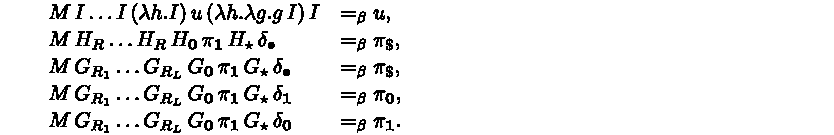
\includegraphics[width=0.95\linewidth,height=0.45\textheight,keepaspectratio]{formula-04.pdf}\end{center}
 
% END Thmtheorem38.p3
 
% END Thmtheorem38
 
% END S3.SSx3.SSS0.P0.SPx2
 
% BEGIN S3.SSx3.SSS0.P0.SPx3
 
\par\medskip\noindent\textbf{Proof.}\par
 
% BEGIN S3.SSx3.SSS0.P0.SPx3.p1
 
The direction from left to right proceeds in two steps. First, by induction on the number of rewriting steps we construct a term $N\in\mathcal{Q}_{n}$ (easy converse of Lemma 34). Second, by induction on $n$ we construct a term $M^{\prime}\in\mathcal{R}_{1}$ containing $N\in\mathcal{Q}_{n}$ as a subterm (easy converse of Lemma 36). Then, the solution is $M:=\lambda r_{1}\ldots r_{L}.\lambda z_{\mathbf{0}}z_{\mathbf{1}}z_{\star}p_{1%
}.M^{\prime}$.\par
 
% END S3.SSx3.SSS0.P0.SPx3.p1
 
% BEGIN S3.SSx3.SSS0.P0.SPx3.p2
 
The direction from right to left proceeds in two steps. First, by Theorem 29 we have $\lambda r_{1}\ldots r_{L}.\lambda z_{\mathbf{0}}z_{\mathbf{1}}z_{\star}p_{1}.M%
^{\prime}$ for some $M^{\prime}\in\mathcal{R}_{1}$. Second, by Lemma 36 and Lemma 34 we have $\mathbf{0}^{n+1}\Rightarrow_{\mathfrak{R}}^{*}\mathbf{1}^{n+1}$ for some $n\in\mathbb{N}$. $\hfill\blacktriangleleft$\par
 
% END S3.SSx3.SSS0.P0.SPx3.p2
 
% BEGIN S3.SSx3.SSS0.P0.SPx3.p3
 
Finally, we present the combination of constraints from the above Lemma 38 as a matching instance $F_{\mathfrak{R}}\,\mathsf{X}=_{\beta}N_{\mathfrak{R}}$. This constitutes the main result of the present work.\par
 
% END S3.SSx3.SSS0.P0.SPx3.p3

% END S3.SSx3.SSS0.P0.SPx3
 
% BEGIN S3.SSx3.SSS0.P0.SPx4
 
\par\medskip\noindent\textbf{Proof.}\par
 
% BEGIN S3.SSx3.SSS0.P0.SPx4.p1
 
Given a simple semi-Thue system $\mathfrak{R}=\{R_{1},\ldots,R_{L}\}$ due to Lemma 38 there exists an $n\in\mathbb{N}$ such that $\mathbf{0}^{n+1}\Rightarrow_{\mathfrak{R}}^{*}\mathbf{1}^{n+1}$ iff the instance $F_{\mathfrak{R}}\,\mathsf{X}=_{\beta}N_{\mathfrak{R}}$ of higher-order $\beta$-matching is solvable, where\par
  
\par\noindent  $\blacksquare$ 
% BEGIN S3.I3.i1.p1
 
\begin{center}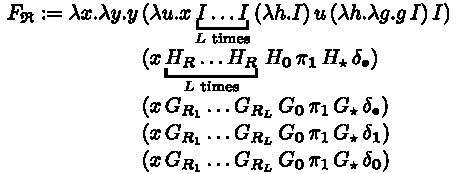
\includegraphics[width=0.95\linewidth,height=0.45\textheight,keepaspectratio]{formula-05.pdf}\end{center}
 
% END S3.I3.i1.p1
 
 
\par\noindent  $\blacksquare$ 
% BEGIN S3.I3.i2.p1
 
$N_{\mathfrak{R}}:=\lambda y.y\,(\lambda u.u)\,\pi_{\$}\,\pi_{\$}\,\pi_{\mathbf%
{0}}\,\pi_{\mathbf{1}}$\par
 
% END S3.I3.i2.p1
 
 
\par\noindent  $\blacksquare$ 
% BEGIN S3.I3.i3.p1
 
$\sigma_{\mathfrak{R}}:=\Gamma_{1}(r_{1})\to\cdots\to\Gamma_{1}(r_{L})\to\Gamma%
_{1}(z_{\mathbf{0}})\to\Gamma_{1}(z_{\mathbf{1}})\to\Gamma_{1}(z_{\star})\to%
\Gamma_{1}(p_{1})\to\kappa$\par
 
% END S3.I3.i3.p1
 
 
\par\noindent  $\blacksquare$ 
% BEGIN S3.I3.i4.p1
 
$\tau_{\mathfrak{R}}:=((\kappa\to\kappa)\to\kappa\to\kappa\to\kappa\to\kappa\to%
\iota)\to\iota$\par
 
% END S3.I3.i4.p1
 
 
\par\noindent  $\blacksquare$ 
% BEGIN S3.I3.i5.p1
 
$\emptyset\vdash F_{\mathfrak{R}}:\sigma_{\mathfrak{R}}\to\tau_{\mathfrak{R}}$\par
 
% END S3.I3.i5.p1
 
 
\par\noindent  $\blacksquare$ 
% BEGIN S3.I3.i6.p1
 
$\emptyset\vdash N_{\mathfrak{R}}:\tau_{\mathfrak{R}}$\par
 
% END S3.I3.i6.p1
 
  
$\hfill\blacktriangleleft$\par
 
% END S3.SSx3.SSS0.P0.SPx4.p1
 
% BEGIN Thmtheorem40
 
\par\medskip\noindent\textbf{Theorem 40.}\par
 
% BEGIN Thmtheorem40.p1
 
Higher-order $\beta$-matching (Problem 7) is undecidable.\par
 
% END Thmtheorem40.p1
 
% END Thmtheorem40
 
% END S3.SSx3.SSS0.P0.SPx4
 
% BEGIN S3.SSx3.SSS0.P0.SPx5
 
\par\medskip\noindent\textbf{Proof.}\par
 
% BEGIN S3.SSx3.SSS0.P0.SPx5.p1
 
By reduction from the undecidable Problem $\mathbf{0}^{+}\Rightarrow^{*}\mathbf{1}^{+}$ (Theorem 17 and Theorem 39). $\hfill\blacktriangleleft$\par
 
% END S3.SSx3.SSS0.P0.SPx5.p1
 
% END S3.SSx3.SSS0.P0.SPx5
 
% END S3.SSx3
 
% END S3

\clearpage
\section*{Complete author formal source for the reduction}
Author library snapshot 70dfc56f33a6e4835281044e68aa68279989047e. Formal code: Mozilla Public License 2.0 (original LICENSE attached). The paper links these proof files; this is collection without a new Coq check. Other named library foundations remain prerequisites of this fixed library version.

\subsection*{L.v}
\begin{lstlisting}
(** * Halting problem for the weak call-by-value lambda-calculus HaltL  *)

(* * The call-by-value lambda calculus L *)

(* ** Syntax   *)

(* The terms of L are the terms of the full lambda-calculus, using de Bruijn encoding  *)
Inductive term : Type :=
| var (n : nat) : term
| app (s : term) (t : term) : term
| lam (s : term).

(* We define a simple, capturing substitution operation *)
Fixpoint subst (s : term) (k : nat) (u : term) :=
  match s with
      | var n => if Nat.eqb n k then u else var n
      | app s t => app (subst s k u) (subst t k u)
      | lam s => lam (subst s (S k) u)
  end.

(* ** Evaluation   *)

(* Big-step evaluation is weak (no evaluations below abstractions) and call-by-value (arguments are fully evaluated when pased) *)
Inductive eval : term -> term -> Prop :=
| eval_abs s : eval (lam s) (lam s)
| eval_app s u t t' v :
    eval s (lam u) -> eval t t' -> eval (subst u 0 t') v -> eval (app s t) v.

(* The L-halting problem  *)
Definition HaltL (s : term) := exists t, eval s t.

(* Scott encoding of natural numbers  *)
Fixpoint nat_enc (n : nat) := 
  match n with
  | 0 => lam (lam (var 1))
  | S n => lam (lam (app (var 0) (nat_enc n)))
  end.

(* ** L-computable relations  *)

Require Import Vector.

Definition L_computable {k} (R : Vector.t nat k -> nat -> Prop) := 
  exists s, forall v : Vector.t nat k, 
      (forall m, R v m <-> L.eval (Vector.fold_left (fun s n => L.app s (nat_enc n)) s v) (nat_enc m)) /\
      (forall o, L.eval (Vector.fold_left (fun s n => L.app s (nat_enc n)) s v) o -> exists m, o = nat_enc m).

Definition closed s := forall n u, subst s n u = s.

Definition L_computable_closed {k} (R : Vector.t nat k -> nat -> Prop) := 
  exists s, closed s /\ forall v : Vector.t nat k, 
      (forall m, R v m <-> L.eval (Vector.fold_left (fun s n => L.app s (nat_enc n)) s v) (nat_enc m)) /\
      (forall o, L.eval (Vector.fold_left (fun s n => L.app s (nat_enc n)) s v) o -> exists m, o = nat_enc m).

\end{lstlisting}

\subsection*{Lambda.v}
\begin{lstlisting}
(*
  Author(s):
    Andrej Dudenhefner (1)
  Affiliation(s):
    (1) TU Dortmund University, Dortmund, Germany
*)

(*
  Problem(s):
    Weak call-by-name leftmost outermost normalization for given closed lambda-terms (wCBNclosed)
    Strong normalization for given closed lambda-terms (SNclosed)

  Literature:
    [1] Plotkin, Gordon.
    "Call-by-name, call-by-value and the λ-calculus."
    Theoretical computer science 1.2 (1975): 125-159.
*)

Require Undecidability.L.L.
Import L (term, var, app, lam).

Require Import Relation_Operators.

(* function composition *)
Definition funcomp {X Y Z} (g : Y -> Z) (f : X -> Y) :=
  fun x => g (f x).

Arguments funcomp {X Y Z} (g f) /.

(* stream cons *)
Definition scons {X : Type} (x : X) (xi : nat -> X) :=
  fun n => match n with | 0 => x | S n => xi n end.

(* parallel term renaming *)
Fixpoint ren (xi : nat -> nat) (t : term) : term  :=
  match t with
  | var x => var (xi x)
  | app s t => app (ren xi s) (ren xi t)
  | lam t => lam (ren (scons 0 (funcomp S xi)) t)
  end.

(* parallel term substitution *)
Fixpoint subst (sigma: nat -> term) (s: term) : term :=
  match s with
  | var n => sigma n
  | app s t => app (subst sigma s) (subst sigma t)
  | lam s => lam (subst (scons (var 0) (funcomp (ren S) sigma)) s)
  end.

Notation closed t := (forall (sigma: nat -> term), subst sigma t = t).

(* beta-reduction (strong call-by-name reduction) *)
Inductive step : term -> term -> Prop :=
  | stepSubst s t   : step (app (lam s) t) (subst (scons t (fun x => var x)) s)
  | stepAppL s s' t : step s s' -> step (app s t) (app s' t)
  | stepAppR s t t' : step t t' -> step (app s t) (app s t')
  | stepLam s s'    : step s s' -> step (lam s) (lam s').

(* given a closed lambda-term s, is it strongly normalizing wrt. beta-reduction? *)
Definition SNclosed : { s : term | closed s } -> Prop :=
  fun '(exist _ s _) => Acc (fun x y => step y x) s.

(* left-most outer-most call-by-name reduction on closed labda-terms *)
Inductive wCBN_step : term -> term -> Prop :=
  | wCBN_stepSubst s t  : wCBN_step (app (lam s) t) (subst (scons t var) s)
  | wCBN_stepApp s s' t : wCBN_step s s' -> wCBN_step (app s t) (app s' t).

(* given a closed lambda-term s, is it normalizing wrt. call-by-name leftmost outermost reduction? *)
Definition wCBNclosed : { s : term | closed s } -> Prop :=
  fun '(exist _ s _) => exists t, clos_refl_trans term wCBN_step s (lam t).

\end{lstlisting}

\subsection*{HOMatching.v}
\begin{lstlisting}
(*
  Author(s):
    Andrej Dudenhefner (TU Dortmund University, Germany)

  Problem(s):
    Higher-Order Matching wrt. beta-equivalence (HOMbeta)

  Literature:
  [1] Loader, Ralph. "Higher order β-matching is undecidable." Logic Journal of the IGPL 11.1 (2003): 51-68.
*)

Require Import List Relation_Operators.

Require Undecidability.L.L Undecidability.LambdaCalculus.Lambda.

(* lambda-term syntax *)
Import L (term, var, app, lam).

(* beta-reduction (strong call-by-name reduction) *)
Import Lambda (step).

(* simple types with a single atom *)
Inductive ty : Type :=
  | atom (* type variable *)
  | arr (s t : ty). (* function type *)

(*
  simply typed lambda-calculus with a single atom
  "stlc Gamma M s" means that in the type environment Gamma the term M is assigned the type s
*)
Inductive stlc (Gamma : list ty) : term -> ty -> Prop :=
  | stlc_var x t : nth_error Gamma x = Some t -> stlc Gamma (var x) t
  | stlc_app M N s t : stlc Gamma M (arr s t) -> stlc Gamma N s -> stlc Gamma (app M N) t
  | stlc_lam M s t : stlc (cons s Gamma) M t -> stlc Gamma (lam M) (arr s t).

(* Higher-Order Matching wrt. beta-equivalence *)
Definition HOMbeta : { '(s, t, F, N) : (ty * ty * term * term) | stlc nil F (arr s t) /\ stlc nil N t } -> Prop :=
  (* given simply typed terms F : s -> t and N : t *)
  fun '(exist _ (s, t, F, N) _) =>
    (* is there a simply typed term M : s such that F A is beta-equivalent to B? *)
    exists (M : term), stlc nil M s /\ clos_refl_sym_trans term step (app F M) N.

\end{lstlisting}

\subsection*{SSTS.v}
\begin{lstlisting}
(* 
  Author(s):
    Andrej Dudenhefner (1) 
  Affiliation(s):
    (1) Saarland University, Saarbrücken, Germany
*)

(* 
  Problem(s):
    Simple Semi-Thue System 01 Rewriting (SSTS01)
*)

(*
  Literature:
  [1] Dudenhefner, Andrej, and Jakob Rehof. 
      "Undecidability of Intersection Type Inhabitation at Rank 3 and its Formalization." 
      Fundamenta Informaticae 170.1-3 (2019): 93-110.
*)

Require Import List Relation_Operators.

(* A simple semi-Thue system consists of rules "ab -> cd" where a, b, c, d : nat *)
Definition Ssts := list ((nat * nat) * (nat * nat)).

(* one-step rewriting relation 
   if (ab -> cd) in ssts, then uabv -> ucdv where u, v : list nat *)
Inductive step (ssts: Ssts) : list nat -> list nat -> Prop := 
  | step_intro {u v: list nat} {a b c d: nat} : 
      In ((a, b), (c, d)) ssts -> step ssts (u ++ a :: b :: v) (u ++ c :: d :: v).

(* reflexive, transitive closure of one-step rewriting *)
Definition multi_step (ssts: Ssts) : list nat -> list nat -> Prop := 
  clos_refl_trans (list nat) (step ssts).

(* simple semi-Thue system 01 rewriting, that is
   for given a simple semi-Thue system, does 0^(1+n) ->> 1^(1+n) hold for some n? *)
Definition SSTS01 : Ssts -> Prop :=
  fun ssts => exists n, multi_step ssts (repeat 0 (1+n)) (repeat 1 (1+n)).
  
\end{lstlisting}

\subsection*{facts.v}
\begin{lstlisting}
Require Import Relations List Lia PeanoNat.
Import ListNotations.
Require Import ssreflect.

#[local] Arguments in_combine_l {A B l l' x y}.
#[local] Arguments app_inj_tail {A x y a b}.

Lemma Forall2_repeat {X Y : Type} (P : X -> Y -> Prop) x y n : P x y -> Forall2 P (repeat x n) (repeat y n).
Proof.
  move=> ?. elim: n; by constructor.
Qed.

Lemma Forall_Forall_impl {X : Type} (P Q : X -> Prop) l : (Forall (fun x => P x -> Q x) l) -> Forall P l -> Forall Q l.
Proof.
  elim; first done.
  move=> > H ? IH /Forall_cons_iff [/H] ??.
  by constructor; auto.
Qed.

Lemma Forall2_repeat_r {X Y : Type} {P : X -> Y -> Prop} {l y n} : Forall2 P l (repeat y n) -> Forall (fun x => P x y) l.
Proof.
  move E: (repeat y n)=> l' H.
  elim: H n E; first done.
  move=> > ?? IH [|n]; first done.
  move=> [? /IH] ?. subst.
  by constructor; auto.
Qed.

Lemma Forall2_repeat_r' {X Y : Type} (P : X -> Y -> Prop) l y n : Forall (fun x => P x y) l -> length l = n -> Forall2 P l (repeat y n).
Proof.
  move=> + <-. elim; first done.
  move=> > ?? IH. by constructor.
Qed.

Lemma nth_error_seq i k : i < k -> nth_error (seq 0 k) i = Some i.
Proof.
  elim: k i; first lia.
  move=> k IH [|i]; first done.
  move=> ? /=.
  rewrite -seq_shift nth_error_map IH; by [|lia].
Qed.

Lemma nth_error_Some' {X : Type} {l : list X} {i : nat} {x : X} : nth_error l i = Some x -> i < length l.
Proof.
  move=> E. apply /nth_error_Some. by rewrite E.
Qed.

Lemma Forall2_change {X Y : Type} (P Q : X -> Y -> Prop) l l1 l2 :
  length l1 = length l2 ->
  (forall i, match (nth_error l i, nth_error l1 i, nth_error l2 i) with (Some x, Some y1, Some y2) => P x y1 -> Q x y2 | _ => True end) ->
  Forall2 P l l1 -> Forall2 Q l l2.
Proof.
  move=> ++ H. elim: H l2; first by case.
  move=> x y1 {}l {}l1 ?? IH [|y2 l2]; first done.
  move=> /= [] /IH {}IH H. constructor; first by apply: (H 0).
  apply: IH=> i. by apply: (H (S i)).
Qed.

Lemma Forall2_change2 {Y : Type} (P Q : nat -> Y -> Prop) m l1 l2 x1 x2 x'1 x'2 :
  (P (length l1) x1 -> Q (length l1) x'1) ->
  (P (S (length l1)) x2 -> Q (S (length l1)) x'2) ->
  (forall i x, i < S (S m) -> i <> length l1 -> i <> S (length l1) -> P i x -> Q i x) ->
  Forall2 P (seq 0 (S (S m))) (l1 ++ x1 :: x2 :: l2) ->
  Forall2 Q (seq 0 (S (S m))) (l1 ++ x'1 :: x'2 :: l2).
Proof.
  move=> Hx1 Hx2 H'. apply: Forall2_change; first by rewrite !length_app.
  move=> i.
  case Ex: (nth_error (seq _ _) i) => [x|]; last done.
  case Ey1: (nth_error (l1 ++ x1 :: x2 :: l2) i) => [y1|]; last done.
  case Ey2: (nth_error (l1 ++ x'1 :: x'2 :: l2) i) => [y2|]; last done.
  move: (Ex) => /nth_error_Some'. rewrite length_seq=> Hx.
  move: Ex. rewrite nth_error_seq; first done.
  move=> [?]. subst i.
  have [?|[?|[??]]] : x = length l1 \/ x = S (length l1) \/ (x <> length l1 /\ x <> S (length l1)) by lia.
  - subst x. move: Ey1. rewrite nth_error_app2; first done.
    rewrite Nat.sub_diag=> - [<-].
    move: Ey2. rewrite nth_error_app2; first done.
    rewrite Nat.sub_diag=> - [<-]. by apply: Hx1.
  - subst x. move: Ey1. rewrite nth_error_app2; first lia.
    have ->: S (length l1) - length l1 = 1 by lia.
    move=> [<-]. move: Ey2. rewrite nth_error_app2; first lia.
    have ->: S (length l1) - length l1 = 1 by lia.
    move=> [<-]. by apply: Hx2.
  - suff ->: y1 = y2 by apply: H'.
    have [?|?] : x < length l1 \/ x > S (length l1) by lia.
    + move: Ey1. rewrite nth_error_app1; first done.
      move: Ey2. rewrite nth_error_app1; first done.
      by move=> -> [<-].
    + move: Ey1 Ey2.
      change (l1 ++ x1 :: x2 :: l2) with (l1 ++ [x1; x2] ++ l2).
      change (l1 ++ x'1 :: x'2 :: l2) with (l1 ++ [x'1; x'2] ++ l2).
      rewrite !app_assoc. rewrite !nth_error_app2 ?length_app /=; [lia..|].
      by move=> -> [<-].
Qed.

Lemma Forall2_map_r {X Y Z : Type} (f : Y -> Z) (P : X -> Z -> Prop) l1 l2 : Forall2 P l1 (map f l2) <-> Forall2 (fun x y => P x (f y)) l1 l2.
Proof.
  split.
  - move E: (map f l2) => l3 H.
    elim: H l2 E; first by case.
    move=> > ??? [|??]; first done.
    move=> /= [??]. subst.
    by auto using Forall2.
  - elim; by constructor.
Qed.

Lemma Forall2_map_l {X Y Z : Type} (f : X -> Z) (P : Z -> Y -> Prop) l1 l2 : Forall2 P (map f l1) l2 <-> Forall2 (fun x y => P (f x) y) l1 l2.
Proof.
  split.
  - move E: (map f l1) => l3 H.
    elim: H l1 E; first by case.
    move=> > ??? [|??]; first done.
    move=> /= [??]. subst.
    by auto using Forall2.
  - elim; by constructor.
Qed.

Lemma Forall2_trans {X Y Z : Type} (P : X -> Y -> Prop) (Q : Y -> Z -> Prop) (R : X -> Z -> Prop) l1 l2 l3 :
  (forall x y z, P x y -> Q y z -> R x z) -> Forall2 P l1 l2 -> Forall2 Q l2 l3 -> Forall2 R l1 l3.
Proof.
  move=> H H'. elim: H' l3.
  - by move=> [|??] /Forall2_length.
  - move=> > ?? IH [|??] /[dup] /Forall2_length; first done.
    move=> _ /Forall2_cons_iff [? /IH ?]. constructor; last done.
    apply: H; by eassumption.
Qed.

\end{lstlisting}

\subsection*{term\_facts.v}
\begin{lstlisting}
(* Key definitions and properties of lambda-terms *)

From Undecidability.L Require L Util.L_facts.
From Undecidability.LambdaCalculus Require Import Lambda Util.facts Util.confluence.
Require Import PeanoNat Lia List Relations.
Import ListNotations.

Import L (term, var, app, lam).
Import L_facts (bound, closed_dcl, dclvar, dclApp, dcllam).

Require Import ssreflect.

Set Default Goal Selector "!".

#[local] Unset Implicit Arguments.

Fixpoint allfv (P : nat -> Prop) t := 
  match t with
  | var x => P x
  | app s t => allfv P s /\ allfv P t
  | lam t => allfv (scons True P) t
  end.

(* P-neutral term *)
Inductive neutral (P : term -> Prop) : term -> Prop :=
  | neutral_var x : neutral P (var x)
  | neutral_app M N : neutral P M -> P N -> neutral P (app M N).

Inductive normal_form : term -> Prop :=
  | normal_var x : normal_form (var x)
  | normal_abs M : normal_form M -> normal_form (lam M)
  | normal_form_app_var x N : normal_form N -> normal_form (app (var x) N)
  | normal_form_app_app M1 M2 N : normal_form (app M1 M2) -> normal_form N -> normal_form (app (app M1 M2) N).

Fixpoint term_size (M : term) :=
  match M with
  | var _ => 1
  | app M' N' => 1 + term_size M' + term_size N'
  | lam M' => 1 + term_size M'
  end.

#[local] Notation sn := (Acc (fun x y => step y x)).
#[local] Notation rt_steps := (clos_refl_trans _ step).
#[local] Notation t_steps := (clos_trans _ step).
#[local] Notation many_app M Ns := (fold_left app Ns M).
#[local] Notation lams k M := (Nat.iter k lam M).

Lemma P_equal {X : Type} (P : X -> Prop) x1 x2 : P x1 -> x2 = x1 -> P x2.
Proof. congruence. Qed.

Lemma clos_trans_flip {X : Type} {R : X -> X -> Prop} {x y} : clos_trans _ R x y ->
  clos_trans _ (fun y x => R x y) y x.
Proof. by elim; eauto using clos_trans. Qed.

Lemma clos_refl_trans_flip {X : Type} {R : X -> X -> Prop} {x y} : clos_refl_trans _ R x y ->
  clos_refl_trans _ (fun y x => R x y) y x.
Proof. by elim; eauto using clos_refl_trans. Qed.

Lemma clos_rt_t' {X : Type} (R : X -> X -> Prop) x y z :
  clos_trans _ R x y -> clos_refl_trans _ R y z -> clos_trans _ R x z.
Proof. move=> H /clos_rt_rtn1_iff H'. elim: H' H; by eauto using clos_trans. Qed.

Lemma neutralE P M : neutral P M ->
  match M with
  | var _ => True
  | app M N => neutral P M /\ P N
  | lam _ => False
  end.
Proof. by case. Qed.

Lemma neutralE' (P : term -> Prop) M : neutral P M -> exists x Ms, M = many_app (var x) Ms /\ Forall P Ms.
Proof.
  elim.
  - move=> x. by exists x, [].
  - move=> {}M N ? [x] [Ms] [->] ??.
    exists x, (Ms ++ [N]). split.
    + by rewrite fold_left_app /=.
    + apply /Forall_app. split; first done.
      by constructor.
Qed.

Lemma ext_ren_term xi1 xi2 t : (forall n, xi1 n = xi2 n) -> ren xi1 t = ren xi2 t.
Proof.
  elim: t xi1 xi2.
  - move=> > /= ?. by congr var.
  - move=> ? IH1 ? IH2 ?? Hxi /=. congr app; [by apply: IH1 | by apply: IH2].
  - move=> ? IH > Hxi /=. congr lam. apply: IH.
    case; first done. move=> ?. by congr S.
Qed.

Lemma ext_subst_term sigma1 sigma2 t : (forall n, sigma1 n = sigma2 n) ->
  subst sigma1 t = subst sigma2 t.
Proof.
  elim: t sigma1 sigma2.
  - by move=> > /= ?.
  - move=> ? IH1 ? IH2 ?? Hsigma /=. congr app; [by apply: IH1 | by apply: IH2].
  - move=> ? IH > Hsigma /=. congr lam. apply: IH.
    case; first done. move=> ?. by rewrite /= Hsigma.
Qed.

Lemma ren_ren_term xi1 xi2 t : ren xi2 (ren xi1 t) = ren (funcomp xi2 xi1) t.
Proof.
  elim: t xi1 xi2 => /=.
  - done.
  - move=> ? IH1 ? IH2 ??. by rewrite IH1 IH2.
  - move=> ? IH ??. rewrite IH.
    congr lam. apply: ext_ren_term. by case.
Qed.

Lemma ren_as_subst_term xi t : ren xi t = subst (funcomp var xi) t.
Proof.
  elim: t xi => /=.
  - done.
  - move=> ? IH1 ? IH2 ?. by rewrite IH1 IH2.
  - move=> ? IH ?. rewrite IH.
    congr lam. apply: ext_subst_term. by case.
Qed.

Lemma ren_subst_term xi sigma t : ren xi (subst sigma t) = subst (funcomp (ren xi) sigma) t.
Proof.
  elim: t xi sigma => /=.
  - done.
  - move=> ? IH1 ? IH2 ??. by rewrite IH1 IH2.
  - move=> ? IH ??. rewrite IH.
    congr lam. apply: ext_subst_term.
    case; first done. move=> ?. by rewrite /= !ren_ren_term.
Qed.

Lemma subst_ren_term xi sigma t : subst sigma (ren xi t) = subst (funcomp sigma xi) t.
Proof.
  elim: t xi sigma => /=.
  - done.
  - move=> ? IH1 ? IH2 ??. by rewrite IH1 IH2.
  - move=> ? IH ??. rewrite IH.
    congr lam. apply: ext_subst_term. by case.
Qed.

Lemma subst_subst_term sigma1 sigma2 t : subst sigma2 (subst sigma1 t) = subst (funcomp (subst sigma2) sigma1) t.
Proof.
  elim: t sigma1 sigma2 => /=.
  - done.
  - move=> ? IH1 ? IH2 ??. by rewrite IH1 IH2.
  - move=> ? IH ??. rewrite IH.
    congr lam. apply: ext_subst_term.
    case; first done. move=> ?.
    by rewrite /= !ren_subst_term !subst_ren_term.
Qed.

Lemma subst_var_term s : subst var s = s.
Proof.
  elim: s.
  - done.
  - move=> ? IH1 ? IH2 /=. by rewrite IH1 IH2.
  - move=> ? IH /=. congr lam. rewrite -[RHS]IH.
    apply: ext_subst_term. by case.
Qed.

Lemma ren_id_term s : ren id s = s.
Proof. by rewrite ren_as_subst_term subst_var_term. Qed.

Definition simpl_term := (ren_ren_term, ren_subst_term, subst_ren_term, subst_subst_term, subst_var_term, ren_id_term).

Lemma allfv_impl (P Q : nat -> Prop) t : 
  (forall x, P x -> Q x) -> allfv P t -> allfv Q t.
Proof.
  elim: t P Q => /=.
  - move=> >. by apply.
  - move=> ? IH1 ? IH2 > /[dup] /IH1 {}IH1 /IH2 {}IH2. tauto.
  - move=> > IH > H /=. apply: IH.
    by case.
Qed.

Lemma ext_allfv_subst_term sigma1 sigma2 t : allfv (fun x=> sigma1 x = sigma2 x) t ->
  subst sigma1 t = subst sigma2 t.
Proof.
  elim: t sigma1 sigma2.
  - by move=> > /= ?.
  - by move=> ? IH1 ? IH2 ?? /= [/IH1 -> /IH2 ->].
  - move=> ? IH > /= Hsigma. congr lam. apply: IH.
    apply: allfv_impl Hsigma.
    by move=> [|x] /= => [|->].
Qed.

Lemma ext_allfv_ren_term xi1 xi2 t : allfv (fun x=> xi1 x = xi2 x) t -> ren xi1 t = ren xi2 t.
Proof.
  move=> H. rewrite !ren_as_subst_term. apply: ext_allfv_subst_term.
  by apply: allfv_impl H => ? /= ->.
Qed.

Lemma boundE k s : bound k s ->
  match s with
  | var n => k > n
  | app s t => bound k s /\ bound k t
  | lam s => bound (S k) s
  end.
Proof. by case. Qed.

Lemma bound_ext_subst_term {k sigma1 sigma2 s} : bound k s -> (forall n, n < k -> sigma1 n = sigma2 n) ->
  subst sigma1 s = subst sigma2 s.
Proof.
  elim: s k sigma1 sigma2.
  - move=> > /boundE /= ?. by apply.
  - move=> ? IH1 ? IH2 k sigma1 sigma2 /boundE + ? /=.
    move=> [/IH1] => /(_ sigma1 sigma2) ->; first done.
    by move=> /IH2 => /(_ sigma1 sigma2) ->.
  - move=> ? IH k sigma1 sigma2 /boundE /IH {}IH H /=. congr lam.
    apply: IH.
    move=> [|n]; first done.
    move=> /= ?. rewrite H; [lia|done].
Qed.

Lemma allfv_closed M : (forall P, allfv P M) -> closed M.
Proof.
  move=> HM sigma. rewrite -[RHS]subst_var_term.
  apply: ext_allfv_subst_term. by apply: HM.
Qed.

Lemma subst_closed sigma M : closed M -> subst sigma M = M.
Proof. by apply. Qed.

Lemma ren_closed xi M : closed M -> ren xi M = M.
Proof. rewrite ren_as_subst_term. by apply. Qed.

Lemma subst_L_closed {sigma t} : L.closed t -> subst sigma t = t.
Proof.
  move=> /closed_dcl /bound_ext_subst_term.
  rewrite -[RHS]subst_var_term. apply. lia.
Qed.

Lemma ren_L_closed {xi t} : L.closed t -> ren xi t = t.
Proof. rewrite ren_as_subst_term. by apply: subst_L_closed. Qed.

Lemma L_subst_Lambda_subst s k t :
  L.closed t -> L.subst s k t = subst (fun n => if Nat.eqb n k then t else var n) s.
Proof.
  move=> Ht. elim: s k.
  - done. 
  - move=> ? IH1 ? IH2 ? /=. by rewrite IH1 IH2.
  - move=> ? IH k /=. rewrite IH.
    congr lam. apply: ext_subst_term.
    move=> [|n] /=; first done.
    case: (Nat.eqb n k); last done.
    by rewrite (ren_L_closed Ht).
Qed.

Lemma bound_ren {k k' xi t} : bound k t -> (forall n, n < k -> xi n < k') -> bound k' (ren xi t).
Proof.
  elim: t k k' xi.
  - move=> > /boundE ? H /=. apply: dclvar. by apply: H.
  - move=> ? IH1 ? IH2 > /boundE + ? /=.
    move=> [/IH1 {}IH1 /IH2 {}IH2]. apply: dclApp; [by apply: IH1|by apply: IH2].
  - move=> ? IH > /boundE /IH {}IH H /=.
    apply: dcllam. apply: IH.
    move=> [|n] /=; [|have := H n]; lia.
Qed.

Lemma bound_subst {k k' sigma t} : bound k t -> (forall n, n < k -> bound k' (sigma n)) -> bound k' (subst sigma t).
Proof.
  elim: t k k' sigma.
  - move=> > /boundE ? H /=. by apply: H.
  - move=> ? IH1 ? IH2 > /boundE + ? /=.
    move=> [/IH1 {}IH1 /IH2 {}IH2]. apply: dclApp; [by apply: IH1|by apply: IH2].
  - move=> ? IH > /boundE /IH {}IH H /=.
    apply: dcllam. apply: IH.
    move=> [|n] /=.
    + move=> _. apply: dclvar. lia.
    + move=> ?. apply: bound_ren; [apply: H|]; lia.
Qed.

Lemma not_closed_var n : L.closed (var n) -> False.
Proof. move=> /(_ n (lam (var 0))) /=. by rewrite Nat.eqb_refl. Qed.

Lemma closed_I s : (forall k, L.subst s k (lam (var 0)) = s) -> L.closed s.
Proof.
  move=> H k u. elim: s k u {H}(H k).
  - move=> /=. move=> n k u. by case: (Nat.eqb n k).
  - by move=> ? IH1 ? IH2 k ? /= [/IH1 -> /IH2 ->].
  - by move=> ? IH k ? /= [/IH ->].
Qed.

Lemma snE M : sn M ->
  match M with
  | var x => True
  | app M N => sn M /\ sn N
  | lam M => sn M
  end.
Proof.
  elim. case.
  - done.
  - move=> M1 M2 IH1 IH2. split.
    + by constructor=> ? /(stepAppL _ _ M2) /IH2 [].
    + by constructor=> ? /(stepAppR M1) /IH2 [].
  - move=> M1 IH1 IH2. by constructor=> ? /stepLam /IH2.
Qed.

Lemma stepE M N : step M N ->
  match M with
  | var _ => False
  | app M1 M2 =>
    (exists M3, M1 = lam M3 /\ N = (subst (scons M2 var) M3)) \/
    (exists M1', step M1 M1' /\ N = app M1' M2) \/
    (exists M2', step M2 M2' /\ N = app M1 M2')
  | lam M => exists M', step M M' /\ N = lam M' 
  end.
Proof.
  case=> *.
  - left. by eexists.
  - right. left. eexists. by split; [eassumption|].
  - right. right. eexists. by split; [eassumption|].
  - eexists. by split; [eassumption|].
Qed.

Lemma normal_form_not_step {M} : normal_form M -> forall N, not (step M N).
Proof.
  elim.
  - by move=> > /stepE.
  - by move=> > _ IH ? /stepE [?] [/IH].
  - move=> > ? IH ? /stepE.
    by move=> [|[|]] [?] [] => [|/stepE|/IH].
  - move=> > _ IH1 _ IH2 ? /stepE.
    by move=> [|[|]] [?] [] => [|/IH1|/IH2].
Qed.

Lemma normal_formE M : normal_form M ->
  match M with
  | var _ => True
  | app M N =>
    match M with
    | var _ => normal_form N
    | app _ _ => normal_form M /\ normal_form N 
    | lam _ => False
    end
  | lam M => normal_form M
  end.
Proof. by case. Qed.

Lemma not_step_normal_form {M} : (forall N, not (step M N)) -> normal_form M.
Proof.
  rewrite /not. elim: M.
  - by do ? constructor.
  - move=> [?|M1 M2|?] IH1 N IH2 H; [..|exfalso].
    all: do ? constructor; by eauto using step.
  - do ? constructor. by eauto using step.
Qed.

Lemma step_dec M : (exists N, step M N) \/ (forall N, not (step M N)).
Proof.
  elim: M.
  - move=> ?. by right=> ? /stepE.
  - move=> M [[M' IH1]|IH1].
    { move=> ? _. left. eexists. apply: stepAppL. by eassumption. }
    move=> N [[N' IH2]|IH2].
    { left. eexists. apply: stepAppR. by eassumption. }
    case: M IH1.
    + move=> > IH1. by right=> ? /stepE [|[|]] [?] [] => [|/IH1|/IH2].
    + move=> > IH1. by right=> ? /stepE [|[|]] [?] [] => [|/IH1|/IH2].
    + move=> *. left. eexists. by apply: stepSubst.
  - move=> M [[??]|IH].
    + left. eexists. apply: stepLam. by eassumption.
    + by right=> ? /stepE [?] [/IH].
Qed.

Lemma normal_form_dec M : (normal_form M) \/ not (normal_form M).
Proof.
  case: (step_dec M).
  - move=> [N] /normal_form_not_step HMN. by right.
  - move=> /not_step_normal_form ?. by left.
Qed.

Lemma t_stepsAppL M M' N : t_steps M M' -> t_steps (app M N) (app M' N).
Proof. by elim; eauto using clos_trans, step. Qed.

Lemma t_stepsAppR M N N' : t_steps N N' -> t_steps (app M N) (app M N').
Proof. by elim; eauto using clos_trans, step. Qed.

Lemma t_stepsLam M M' : t_steps M M' -> t_steps (lam M) (lam M').
Proof. by elim; eauto using clos_trans, step. Qed.

Lemma rt_stepsAppL M M' N :rt_steps M M' -> rt_steps (app M N) (app M' N).
Proof. by elim; eauto using clos_refl_trans, step. Qed.

Lemma rt_stepsAppR M N N' : rt_steps N N' -> rt_steps (app M N) (app M N').
Proof. by elim; eauto using clos_refl_trans, step. Qed.

Lemma rt_stepsLam M M' : rt_steps M M' -> rt_steps (lam M) (lam M').
Proof. by elim; eauto using clos_refl_trans, step. Qed.

Lemma ren_step xi M M' : step M M' -> step (ren xi M) (ren xi M').
Proof.
  move=> H. elim: H xi; [|by eauto using step..].
  move=> > /=. apply: P_equal; [by apply: stepSubst|].
  rewrite !simpl_term. apply: ext_subst_term. by case.
Qed.

Lemma subst_step M N sigma : step M N ->
  step (subst sigma M) (subst sigma N).
Proof.
  move=> H. elim: H sigma; [|by eauto using step..].
  move=> > /=.
  apply: P_equal; [apply: stepSubst|].
  rewrite !simpl_term. apply: ext_subst_term=> - [|?]; [done|].
  by rewrite /= !simpl_term.
Qed.

Lemma ren_steps xi M M' : clos_refl_trans _ step M M' ->
  clos_refl_trans _ step (ren xi M) (ren xi M').
Proof. by elim; eauto using clos_refl_trans, ren_step. Qed.

Lemma subst_steps sigma sigma' M : (forall n, clos_refl_trans _ step (sigma n) (sigma' n)) ->
  clos_refl_trans _ step (subst sigma M) (subst sigma' M).
Proof.
  elim: M sigma sigma'.
  - move=> ???. by apply.
  - move=> * /=. apply: rt_trans; [apply: rt_stepsAppR|apply: rt_stepsAppL]; by auto.
  - move=> ? IH * /=. apply: rt_stepsLam. apply: IH.
    move=> [|?] /=; [by apply rt_refl|].
    by apply: ren_steps.
Qed.

(* weak normalization property *)
Inductive wn M : Prop :=
  | wn_intro N : clos_refl_trans term step M N -> normal_form N -> wn M.

Arguments wn_intro {M}.

Lemma allfv_trivial (P : nat -> Prop) t : (forall x, P x) -> allfv P t.
Proof.
  elim: t P=> /=; [by auto..|].
  move=> ? IH *. by apply: IH => - [|?].
Qed.

Lemma allfv_allfv_impl (P Q : nat -> Prop) t : 
  allfv (fun x => P x -> Q x) t -> allfv P t -> allfv Q t.
Proof.
  elim: t P Q => /=.
  - move=> >. by apply.
  - move=> ? IH1 ? IH2 > [/IH1 {}IH1] /IH2 {}IH2.
    by move=> [/IH1] {}IH1 /IH2 {}IH2.
  - move=> ? > IH > H /=. apply: IH.
    apply: allfv_impl H. by case.
Qed.

Lemma allfv_dec P M : (forall x, P x \/ not (P x)) -> allfv P M \/ not (allfv P M).
Proof.
  elim: M P=> /=.
  - done.
  - move=> s IH1 t IH2 ? /[dup] /IH1 {}IH1 /IH2 {}IH2. tauto.
  - move=> ? IH P H.
    case: (IH (scons True P)); [|by auto..].
    move=> [|?] /=; by auto.
Qed.

Lemma allfv_ren (P : nat -> Prop) xi t :
  allfv (funcomp P xi) t ->  allfv P (ren xi t).
Proof.
  elim: t P xi.
  - done.
  - move=> ? IH1 ? IH2 > /= [??]. by auto.
  - move=> ? IH > /= H. apply: IH.
    by apply: allfv_impl H => - [|?].
Qed.

Lemma allfv_ren' (P : nat -> Prop) xi t :
  allfv P (ren xi t) -> allfv (funcomp P xi) t.
Proof.
  elim: t P xi.
  - done.
  - move=> ? IH1 ? IH2 > /= [??]. split.
    + by apply: IH1.
    + by apply: IH2.
  - move=> ? IH > /= /IH.
    by apply: allfv_impl => - [|?].
Qed.

Lemma allfv_subst (P : nat -> Prop) sigma t :
  allfv (fun x => allfv P (sigma x)) t ->  allfv P (subst sigma t).
Proof.
  elim: t P sigma.
  - done.
  - move=> ? IH1 ? IH2 > /= [??]. by auto.
  - move=> ? IH > /= H. apply: IH.
    apply: allfv_impl H => - [|?] /= H; [done|].
    apply: allfv_ren. by apply: allfv_impl H. 
Qed.

Lemma allfv_subst' (P : nat -> Prop) sigma t :
  allfv P (subst sigma t) -> allfv (fun x => allfv P (sigma x)) t.
Proof.
  elim: t P sigma.
  - done.
  - move=> ? IH1 ? IH2 > /= [??]. by auto.
  - move=> ? IH > /= /IH.
    apply: allfv_impl => - [|?] /=; [done|].
    move=> /allfv_ren'. by apply: allfv_impl.
Qed.

Lemma stepSubst' s t u : u = subst (scons t var) s -> step (app (lam s) t) u.
Proof. move=> ->. by apply: stepSubst. Qed.

Lemma subst_as_ren M x : subst (scons (var x) var) M = ren (scons x id) M.
Proof.
  rewrite ren_as_subst_term /=. apply: ext_subst_term. by case.
Qed.

Lemma step_ren xi M N : step M N -> step (ren xi M) (ren xi N).
Proof.
  move=> H. elim: H xi.
  { move=> > /=.
    apply: stepSubst'.
    rewrite !simpl_term. apply: ext_subst_term.
    by case. }
  all: by eauto using step with nocore.
Qed.

Fact normal_form_ren xi M : 
  normal_form M -> normal_form (ren xi M).
Proof.
  move=> H. elim: H xi; cbn; by eauto using normal_form.
Qed.

Fact normal_form_ren' xi M : 
  normal_form (ren xi M) -> normal_form M.
Proof.
  elim: M xi=> /=.
  - by eauto using normal_form.
  - move=> [?|??|?] /= IH1 ? IH2 ? /normal_formE.
    + by eauto using normal_form.
    + move=> [??]. by eauto using normal_form.
    + done.
  - move=> ??? /normal_formE. by eauto using normal_form.
Qed.

Lemma step_renE xi M N : step (ren xi M) N -> exists N', N = ren xi N' /\ step M N'.
Proof.
  move E: (ren xi M) => M' H. elim: H xi M E.
  - move=> ??? [] //.
    move=> [] // ?? /= [<- <-]. eexists.
    split; first last. { by apply: stepSubst. }
    rewrite !simpl_term. apply: ext_subst_term.
    by case.
  - move=> > ? IH ? [] //= ?? [??]. subst.
    have [? [? ?]] := IH _ _ eq_refl. subst.
    eexists.
    split; first last. { apply: stepAppL. eassumption. }
    done.
  - move=> > ? IH ? [] //= ?? [??]. subst.
    have [? [? ?]] := IH _ _ eq_refl. subst.
    eexists.
    split; first last. { apply: stepAppR. eassumption. }
    done.
  - move=> > ? IH ? [] //= ? [?]. subst.
    have [? [? ?]] := IH _ _ eq_refl. subst.
    eexists.
    split; first last. { apply: stepLam. eassumption. }
    done.
Qed.

Lemma steps_renE xi M N : clos_refl_trans term step (ren xi M) N -> exists N', N = ren xi N' /\ clos_refl_trans term step M N'.
Proof.
  move E: (ren xi M) => M' /clos_rt_rt1n_iff H.
  elim: H xi M E.
  { move=> > <-. eexists. split;[done|]. by apply: rt_refl. }
  move=> > +++ > ?. subst. move=> /step_renE [?] [->] ? _.
  move=> /(_ _ _ eq_refl) [?] [->] ?.
  eexists. split; [done|].
  apply: rt_trans; [apply: rt_step|]; eassumption.
Qed.

Lemma term_size_many_app M Ns : term_size (many_app M Ns) = list_sum (map (fun N => S (term_size N)) Ns) + term_size M.
Proof.
  elim: Ns M.
  - done.
  - move=> ?? IH ? /=. rewrite IH /=. lia.
Qed.

Lemma neutral_normal_form M :
  neutral normal_form M -> normal_form M.
Proof.
  elim.
  - by constructor.
  - move=> > []; do ? constructor; by auto.
Qed.

Lemma normal_form_neutral M : normal_form M ->
  neutral normal_form M \/
  (exists N, M = lam N /\ normal_form N).
Proof.
  elim.
  - move=> >. left. by constructor.
  - move=> *. right. by do ? econstructor.
  - move=> *. left. by do ? constructor.
  - move=> > ? [?| [? [??]]]; [|done].
    left. by constructor.
Qed.

Lemma normal_form_app_neutral M N : normal_form (app M N) -> neutral normal_form (app M N).
Proof. by move=> > /normal_form_neutral [?|[?] [??]]. Qed.

Lemma neutral_impl (P Q : term -> Prop) M :
  (forall N, P N -> Q N) ->
  neutral P M -> neutral Q M.
Proof. move=> H. elim; by auto using neutral. Qed.

Lemma neutral_dec P M : (forall M, P M \/ not (P M)) ->
  neutral P M \/ not (neutral P M).
Proof.
  move=> H. elim: M.
  - left. by constructor.
  - move=> M [].
    + move=> ? N _. case: (H N).
      * left. by constructor.
      * move=> ?. by right => /neutralE [].
    + move=> *. by right => /neutralE [].
  - by right=> /neutralE.
Qed.

Lemma ren_many_app xi M Ns : ren xi (many_app M Ns) = many_app (ren xi M) (map (ren xi) Ns).
Proof. elim: Ns M; [done|]. move=> > IH ? /=. by rewrite IH. Qed.

Lemma subst_many_app sigma M Ns : subst sigma (many_app M Ns) = many_app (subst sigma M) (map (subst sigma) Ns).
Proof. elim: Ns M; [done|]. move=> > IH ? /=. by rewrite IH. Qed.

Lemma normal_form_steps N M : normal_form N -> rt_steps N M -> N = M. 
Proof.
  move=> /normal_form_not_step H /clos_rt_rt1n_iff H'.
  case: H' H; first done.
  by move=> > + _ H => /H.
Qed.

Lemma ren_apps xi M Ns : ren xi (many_app M Ns) = many_app (ren xi M) (map (ren xi) Ns).
Proof.
  elim: Ns M; first done.
  move=> ?? IH M /=. by rewrite IH.
Qed.

Lemma subst_apps sigma M Ns : subst sigma (many_app M Ns) = many_app (subst sigma M) (map (subst sigma) Ns).
Proof.
  elim: Ns M; first done.
  move=> ?? IH M /=. by rewrite IH.
Qed.

Lemma allfv_step P M N : step M N -> allfv P M -> allfv P N.
Proof.
  move=> H. elim: H P.
  - move=> /= > [HM HN]. apply: allfv_subst.
    apply: allfv_impl HM. by case.
  - by move=> > ? IH ? /= [/IH ??].
  - by move=> > ? IH ? /= [? /IH ?].
  - move=> > ? IH ?. by apply: IH.
Qed.

Lemma allfv_steps P M N : rt_steps M N -> allfv P M -> allfv P N.
Proof.
  elim.
  - move=> > /allfv_step. by apply.
  - done.
  - by auto.
Qed.

Lemma allfv_apps P M Ms : allfv P M -> Forall (allfv P) Ms -> allfv P (many_app M Ms).
Proof.
  elim: Ms M; first done.
  move=> M' Ms IH M ? /Forall_cons_iff [? /IH] /=. by apply.
Qed.

Lemma allfv_lams P n M : allfv (Nat.iter n (scons True) P) M -> allfv P (lams n M).
Proof.
  elim: n P; first done.
  move=> n IH P.
  rewrite Nat.iter_succ_r.
  by apply: IH.
Qed.

Lemma steps_ren xi M N : rt_steps M N -> rt_steps (ren xi M) (ren xi N).
Proof.
  elim=> *.
  - apply: rt_step. by apply: step_ren.
  - by apply: rt_refl.
  - apply: rt_trans; by eassumption.
Qed.

Lemma steps_ren' xi M N : rt_steps (ren xi M) N -> exists N', N = ren xi N' /\ rt_steps M N'.
Proof.
  move=> /clos_rt_rtn1_iff. elim.
  - exists M. by split; [|apply: rt_refl].
  - move=> > H ? [?] [??]. subst.
    move: H=> /step_renE [?] [??]. subst.
    eexists. subst. split; first done.
    by apply: rt_trans; [|apply: rt_step]; eassumption.
Qed.

Lemma steps_subst sigma M N : rt_steps M N -> rt_steps (subst sigma M) (subst sigma N).
Proof.
  elim=> *.
  - apply: rt_step. by apply: subst_step.
  - by apply: rt_refl.
  - apply: rt_trans; by eassumption.
Qed.

Lemma stepsAppL N M M' : rt_steps M M' -> rt_steps (app M N) (app M' N).
Proof.
  elim=> *.
  - apply: rt_step. by apply: stepAppL.
  - by apply: rt_refl.
  - apply: rt_trans; by eassumption.
Qed.

Lemma stepsAppR N M M' : rt_steps M M' -> rt_steps (app N M) (app N M').
Proof.
  elim=> *.
  - apply: rt_step. by apply: stepAppR.
  - by apply: rt_refl.
  - apply: rt_trans; by eassumption.
Qed.

Lemma stepsLam M M' : rt_steps M M' -> rt_steps (lam M) (lam M').
Proof.
  elim=> *.
  - apply: rt_step. by apply: stepLam.
  - by apply: rt_refl.
  - apply: rt_trans; by eassumption.
Qed.

Lemma steps_subst' sigma sigma' M : (forall x, rt_steps (sigma x) (sigma' x)) -> rt_steps (subst sigma M) (subst sigma' M).
Proof.
  elim: M sigma sigma'.
  - move=> >. by apply.
  - move=> M IHM N IHN > H /=. apply: rt_trans.
    + apply: stepsAppL. apply IHM. by eassumption.
    + apply: stepsAppR. apply IHN. by eassumption.
  - move=> M IH > H /=. apply stepsLam. apply: IH.
    move=> [|x] /=; first by apply: rt_refl.
    apply: steps_ren. by apply: H.
Qed.

Lemma steps_subst'' sigma sigma' M M' : (forall x, rt_steps (sigma x) (sigma' x)) -> rt_steps M M' -> rt_steps (subst sigma M) (subst sigma' M').
Proof.
  move=> H /(steps_subst sigma'). apply: rt_trans. by apply: steps_subst'.
Qed.

Lemma stepAppsL M M' Ns : step M M' -> step (many_app M Ns) (many_app M' Ns).
Proof.
  move: M M'.
  elim: Ns; first done.
  move=> N Ns IH /= M M' H. apply: IH. by apply: stepAppL.
Qed.

Lemma stepsAppsL M M' Ns : rt_steps M M' -> rt_steps (many_app M Ns) (many_app M' Ns).
Proof.
  elim=> *.
  - apply: rt_step. by apply: stepAppsL.
  - apply: rt_refl.
  - apply: rt_trans; by eassumption.
Qed.

Lemma stepsAppsR M Ms M's : Forall2 rt_steps Ms M's -> rt_steps (many_app M Ms) (many_app M M's).
Proof.
  move=> H. elim: H M; first by apply: rt_refl.
  move=> > ?? IH M /=.
  apply: rt_trans.
  { apply: stepsAppsL. apply: stepsAppR. by eassumption. }
  by apply: IH.
Qed.

Lemma stepsLams k M M' : rt_steps M M' -> rt_steps (lams k M) (lams k M').
Proof.
  move=> ?. elim: k; first done.
  move=> *. rewrite /=. apply: stepsLam. by eassumption.
Qed.

Definition up (sigma: nat -> term) := scons (var 0) (funcomp (ren S) sigma).

Lemma subst_lams sigma k M : subst sigma (lams k M) = lams k (subst (Nat.iter k up sigma) M).
Proof.
  elim: k sigma M; first done.
  move=> k IH sigma M.
  rewrite !Nat.iter_succ_r /=.
  rewrite IH /=. congr (lams _ _).
  by rewrite -Nat.iter_succ_r /=.
Qed.

Lemma steps_refl M N : M = N -> rt_steps M N.
Proof.
  move=> <-. by apply: rt_refl.
Qed.

Lemma stepsReds M Ns : rt_steps (many_app (lams (length Ns) M) Ns) (subst (fold_left (fun sigma N => scons N sigma) Ns var) M).
Proof.
  suff: forall sigma, rt_steps (many_app (lams (length Ns) (subst (Nat.iter (length Ns) up sigma) M)) Ns) (subst (fold_left (fun sigma N => scons N sigma) Ns sigma) M).
  { move=> /(_ var) H. apply: rt_trans; [|by apply: H].
    apply: steps_refl. congr (many_app _ _). congr (lams _ _).
    rewrite -[LHS]subst_var_term. apply: ext_subst_term.
    elim: Ns {H}; first done.
    move=> N Ns IH [|x] /=; first done.
    by rewrite -IH. }
  elim: Ns M.
  - move=> ? sigma /=. by apply: rt_refl.
  - move=> N Ns IH M sigma /=.
    apply: rt_trans.
    + apply: stepsAppsL. apply: rt_step. by apply: stepSubst.
    + apply: rt_trans; [|by apply: IH]. apply: steps_refl.
      rewrite subst_lams. congr (many_app _ _). congr (lams _ _).
      rewrite subst_subst_term. apply: ext_subst_term.
      move: sigma {IH}. elim: Ns.
      { move=> sigma [|x] /=; first done.
        rewrite subst_ren_term. by apply: subst_var_term. }
      move=> n' Ns IH sigma [|x] /=; first done.
      by rewrite -IH subst_ren_term ren_subst_term /=.
Qed.

Lemma iter_up_lt k x sigma : x < k -> Nat.iter k up sigma x = var x.
Proof.
  elim: k sigma x.
  - lia.
  - move=> k IH sigma [|x] ? /=; first done.
    change (var (S x)) with (ren S (var x)).
    congr ren. apply: IH. lia.
Qed.

Lemma iter_up_ge k x sigma : x >= k -> Nat.iter k up sigma x = ren (fun y => k + y) (sigma (x - k)).
Proof.
  elim: k sigma x.
  - move=> *. by rewrite Nat.sub_0_r ren_id_term. 
  - move=> k IH sigma [|x] ? /=; first by lia.
    rewrite IH; first by lia.
    by rewrite ren_ren_term.
Qed.

Lemma iter_up_eq (x : nat) (sigma : nat -> term) :
  Nat.iter x up sigma x = ren (Nat.add x) (sigma 0).
Proof.
  by rewrite iter_up_ge ?Nat.sub_diag.
Qed.

Lemma apps_apps M M1s M2s : many_app (many_app M M1s) M2s = many_app M (M1s ++ M2s).
Proof.
  elim: M1s M; first done.
  move=> > + ?. by apply.
Qed.

Lemma lams_lams k1 k2 M : lams k1 (lams k2 M) = lams (k1 + k2) M.
Proof.
  elim: k1; first done.
  by move=> ? /= ->.
Qed.

Lemma stepsRed M N : rt_steps (app (lam M) N) (subst (scons N var) M).
Proof. apply: rt_step. by apply: stepSubst. Qed.

Lemma stepsReds' k (M : term) (Ns : list term) : length Ns = k ->
  rt_steps (many_app (lams k M) Ns) (subst (fold_left (fun sigma N => scons N sigma) Ns var) M).
Proof. move=> <-. by apply: stepsReds. Qed.

Lemma allfv_var (P : nat -> Prop) (x : nat) : P x -> allfv P (var x).
Proof. done. Qed.

Lemma allfv_app P M1 M2 : allfv P M1 -> allfv P M2 -> allfv P (app M1 M2).
Proof.
  move=> *. by split.
Qed.

Lemma apps_inj M Ms M's : many_app M Ms = many_app M M's -> Ms = M's.
Proof.
  elim /rev_ind: Ms M M's.
  - move=> ? [|??]; first done.
    move=> /(f_equal term_size) /=. rewrite term_size_many_app /=. lia.
  - move=> > IH ? M's. elim /rev_ind: M's.
    + move=> /(f_equal term_size) /=. rewrite term_size_many_app map_app list_sum_app /=. lia.
    + move=> ?? _. rewrite !fold_left_app /=.
      by move=> [] /IH <- <-.
Qed.

Lemma Forall2_steps_refl Ms : Forall2 rt_steps Ms Ms.
Proof.
  elim: Ms; first done.
  move=> *. constructor; last done.
  by apply: rt_refl.
Qed.

Lemma apps_last M Ms N : many_app M (Ms ++ [N]) = app (many_app M Ms) N.
Proof. by rewrite fold_left_app. Qed.

Lemma step_apps_varE x Ms M : step (many_app (var x) Ms) M -> exists M's, M = many_app (var x) M's /\ Forall2 rt_steps Ms M's.
Proof.
  move E: (many_app (var x) Ms) => M' H. elim: H Ms E.
  - move=> ?? Ms. elim /rev_ind: Ms; first done.
    move=> ? M's _. rewrite apps_last.
    move=> []. elim /rev_ind: M's; first done.
    move=> ?? _. by rewrite apps_last.
  - move=> > ? IH Ms. elim /rev_ind: Ms; first done.
    move=> ?? _. rewrite apps_last.
    move=> [??]. subst.
    move: (IH _ eq_refl) => [M's] [??]. subst.
    eexists. split; first by rewrite -apps_last.
    apply: Forall2_app; first done.
    by apply: Forall2_steps_refl.
  - move=> > ? IH Ms. elim /rev_ind: Ms; first done.
    move=> ? M's _. rewrite apps_last.
    move=> [??]. subst.
    eexists. split; first by rewrite -apps_last.
    apply: Forall2_app.
    + by apply: Forall2_steps_refl.
    + constructor; last done. by apply: rt_step.
  - move=> > ?? Ms. elim /rev_ind: Ms; first done.
    move=> > _. by rewrite apps_last.
Qed.

Lemma steps_apps_varE x Ms M's : rt_steps (many_app (var x) Ms) (many_app (var x) M's) -> Forall2 rt_steps Ms M's.
Proof.
  move E: (many_app (var x) Ms)=> M.
  move E': (many_app (var x) M's)=> M' /clos_rt_rt1n_iff H.
  elim: H Ms M's E E'.
  - move=> ? Ms M's <- /apps_inj <-.
    by apply: Forall2_steps_refl.
  - move=> > H ? IH > ??. subst.
    move: H => /step_apps_varE [M's] [?] H. subst.
    apply: Forall2_trans H (IH _ _ eq_refl eq_refl).
    move=> >. by apply: rt_trans.
Qed.

Lemma step_lamE M N : step (lam M) N -> match N with lam N' => step M N' | _ => False end.
Proof.
  intros H. by inversion H; subst.
Qed.

Lemma steps_lamE M N : rt_steps (lam M) N -> match N with lam N' => rt_steps M N' | _ => False end.
Proof.
  move E: (lam M) => M' /clos_rt_rt1n_iff H.
  elim: H M E.
  - move=> ?? <-. by apply: rt_refl.
  - move=> ? {}M M'' H _ IH ??. subst.
    move=> /step_lamE in H.
    move: M H IH=> [?|??|?]; [done..|].
    move=> ? /(_ _ eq_refl).
    move: M''=> [?|??|?]; [done..|].
    move=> ?. by apply: rt_trans; [apply: rt_step|]; eassumption.
Qed.

Lemma steps_lamsE k M N : rt_steps (lams k M) (lams k N) -> rt_steps M N.
Proof.
  elim: k; first done.
  by move=> k IH /= /steps_lamE /IH.
Qed.

Lemma steps_var_absurd (P : Prop) M x : allfv (fun y => y <> x) M -> rt_steps M (var x) -> P.
Proof.
  by move=> /allfv_steps /[apply].
Qed.

Lemma subst_lam sigma M : subst sigma (lam M) = lam (subst (up sigma) M).
Proof. done. Qed.

Lemma allfv_ren_lt i n M :
  i < n -> allfv (fun y : nat => y <> i) (ren (Nat.add n) M).
Proof.
  move=> ?. apply: allfv_ren. apply: allfv_trivial.
  move=> /=. lia.
Qed.

Module Confluence.
(* parallel reduction *)
Inductive par : term -> term -> Prop :=
  | par_var x : par (var x) (var x)
  | par_lam M M' : par M M' -> par (lam M) (lam M')
  | par_step M M' N N': par M M' -> par N N' -> par (app (lam M) N) (subst (scons N' var) M')
  | par_app M M' N N': par M M' -> par N N' -> par (app M N) (app M' N').

Lemma par_step' M M' N N' T : par M M' -> par N N' -> T = (subst (scons N' var) M') -> par (app (lam M) N) T.
Proof.
  intros ?? ->. now apply par_step.
Qed.

Lemma reflexive_par : reflexive term par.
Proof.
  intros M. now induction M; auto using par.
Qed.

Lemma inclusion_step_par : inclusion term step par.
Proof.
  intros M N H. now induction H; auto using par, reflexive_par.
Qed.

Lemma inclusion_par_steps : inclusion term par rt_steps.
Proof.
  intros M N H. induction H.
  - now apply rt_refl.
  - now apply stepsLam.
  - eapply rt_trans.
    + apply rt_step. now apply stepSubst.
    + apply steps_subst''; [|assumption].
      intros [|x]; [assumption|].
      apply rt_refl.
  - eapply rt_trans.
    + apply stepsAppL. eassumption.
    + apply stepsAppR. eassumption.
Qed.

Fixpoint rho (M : term) :=
  match M with
  | var x => var x
  | lam M => lam (rho M)
  | app (lam M) N => subst (scons (rho N) var) (rho M)
  | app M N => app (rho M) (rho N)
  end.

Lemma par_ren xi M M' : par M M' -> par (ren xi M) (ren xi M').
Proof.
  intros H. revert xi. induction H; intros xi; cbn.
  - now apply par_var.
  - now apply par_lam; auto.
  - eapply par_step'; [auto..|].
    rewrite ren_subst_term subst_ren_term.
    apply ext_subst_term. now intros [|x].
  - now apply par_app; auto.
Qed.

Lemma par_subst sigma sigma' M M' : (forall x, par (sigma x) (sigma' x)) -> par M M' -> par (subst sigma M) (subst sigma' M').
Proof.
  intros E H. revert sigma sigma' E.
  induction H as [x|M M' H IH|M M' N N' H1 IH1 H2 IH2|M M' N N' H1 IH1 H2 IH2].
  - intros ?? E. now apply E.
  - intros ?? E. cbn. apply par_lam. apply IH.
    intros [|x]; cbn.
    + now apply reflexive_par.
    + apply par_ren. now apply E.
  - intros ?? E. cbn. eapply (par_step' _ (subst (up sigma') M') _ (subst sigma' N')).
    + apply IH1. intros [|x]; cbn.
      * apply reflexive_par.
      * apply par_ren. apply E.
    + apply IH2. apply E.
    + rewrite !subst_subst_term. apply ext_subst_term. intros [|x]; cbn.
      * easy.
      * now rewrite subst_ren_term subst_var_term.
  - intros ?? E. cbn. apply par_app.
    + now apply IH1.
    + now apply IH2.
Qed.

Lemma tak_fun_par_rho : tak_fun term par rho.
Proof.
  intros M N H.
  induction H as [x|M M' H IH|M M' N N' H1 IH1 H2 IH2|M M' N N' H1 IH1 H2 IH2]; cbn.
  - now apply par_var.
  - now apply par_lam.
  - apply par_subst; [|assumption].
    intros [|x]; [assumption|].
    apply reflexive_par.
  - destruct M.
    + now apply par_app.
    + now apply par_app.
    + inversion H1. subst. apply par_step; [|assumption].
      inversion IH1. now subst.
Qed.
End Confluence.

Lemma confluence_step: confluent step.
Proof.
  eapply TMT.
  - apply Confluence.inclusion_step_par.
  - apply Confluence.inclusion_par_steps.
  - apply Confluence.reflexive_par.
  - apply Confluence.tak_fun_par_rho.
Qed.

Lemma steps_nf_elim {P : Prop} {M M' N : term} : normal_form N -> rt_steps M M' -> (rt_steps M' N -> P) -> rt_steps M N -> P.
Proof.
  move=> HN /confluence_step HM H /HM [N'] [H'] H''. apply: H.
  apply: rt_trans; first by eassumption.
  move: H'' HN => /clos_rt_rt1n_iff [].
  - move=> *. by apply: rt_refl.
  - by move=> > /normal_form_not_step.
Qed.

Lemma steps_var_elim {P : Prop} {M M' : term} {x : nat} : rt_steps M M' -> (rt_steps M' (var x) -> P) -> rt_steps M (var x) -> P.
Proof.
  apply: steps_nf_elim. by do 2 constructor.
Qed.

Module TermNotations.
(* strong normalization *)
Notation sn := (Acc (fun x y => step y x)).
(* reflexive, transite closure of step *)
Notation rt_steps := (clos_refl_trans _ step).
(* transite closure of step *)
Notation t_steps := (clos_trans _ step).
(* iterated term application *)
Notation many_app M Ns := (fold_left app Ns M).
End TermNotations.

\end{lstlisting}

\subsection*{stlc\_facts.v}
\begin{lstlisting}
(*
  facts about the simplty typed lambda-calculus
*)

Require Import Lia List Relations PeanoNat.
Import ListNotations.

Require Undecidability.L.L.
Import L (term, var, app, lam).

From Undecidability.LambdaCalculus Require Import Lambda HOMatching Util.facts Util.term_facts.
Require Import ssreflect ssrbool.

#[local] Unset Implicit Arguments.

Set Default Goal Selector "!".

#[local] Notation lams k M := (Nat.iter k lam M).
#[local] Notation apps M Ns := (fold_left app Ns M).
#[local] Notation arrs ss t := (fold_right arr t ss).
#[local] Notation steps := (clos_refl_trans _ step).

Fixpoint ty_size (t : ty) : nat :=
  match t with
  | atom => 1
  | arr s t => 1 + ty_size s + ty_size t
  end.

Lemma ty_size_arrs ss B : ty_size (arrs ss B) = list_sum (map (fun s => 1 + ty_size s) ss) + ty_size B.
Proof.
  elim: ss; first done.
  move=> ?? IH /=. rewrite IH /=. lia.
Qed.

Lemma arrs_inj s1s s2s t : arrs s1s t = arrs s2s t -> s1s = s2s.
Proof.
  elim: s1s s2s.
  - move=> [|??]; first done.
    move=> /= /(f_equal ty_size) /=. rewrite ty_size_arrs. lia.
  - move=> ?? IH [|??].
    + move=> /= /(f_equal ty_size) /=. rewrite ty_size_arrs. lia.
    + by move=> [<-] /IH <-.
Qed.

Lemma arrs_arrs s1s s2s t : arrs s1s (arrs s2s t) = arrs (s1s ++ s2s) t.
Proof.
  by rewrite fold_right_app.
Qed.

Inductive stlc_app_spec (Gamma : list ty) (t : ty) (M N : term) : Prop :=
  | stlc_app_spec_intro s : stlc Gamma M (arr s t) -> stlc Gamma N s -> stlc_app_spec Gamma t M N.
Inductive stlc_lam_spec (Gamma : list ty) (t : ty) (M : term) : Prop :=
  | stlc_lam_spec_intro s' t' : t = arr s' t' -> stlc (cons s' Gamma) M t' -> stlc_lam_spec Gamma t M.

Lemma stlcE Gamma M t : stlc Gamma M t ->
  match M with
  | var x => nth_error Gamma x = Some t
  | app M N => stlc_app_spec Gamma t M N
  | lam M => stlc_lam_spec Gamma t M
  end.
Proof. case; [|econstructor..]; by eauto. Qed.

Lemma stlc_appsE Gamma M Ns t : stlc Gamma (apps M Ns) t ->
  exists ss, Forall2 (stlc Gamma) Ns ss /\ stlc Gamma M (arrs ss t).
Proof.
  elim: Ns M t.
  - move=> M t /= ?. by exists [].
  - move=> N Ns IH M t /= /IH [ss] [?].
    move=> /stlcE [] s *. exists (s :: ss). by split; [constructor|].
Qed.

Lemma stlc_lamsE Gamma M ss B : stlc Gamma (lams (length ss) M) (arrs ss B) -> stlc (rev ss ++ Gamma) M B.
Proof.
  elim: ss Gamma; first done.
  move=> ?? IH ? /= /stlcE [] ?? [<- <-] /IH.
  by rewrite -app_assoc.
Qed.

Lemma stlc_lamsE' Gamma M n ss B : n = length ss -> stlc Gamma (lams n M) (arrs ss B) -> stlc (rev ss ++ Gamma) M B.
Proof. move=> ->. by apply: stlc_lamsE. Qed.

Lemma stlc_allfv_ren Gamma Delta xi M t : allfv (fun x => forall s, nth_error Gamma x = Some s -> nth_error Delta (xi x) = Some s) M ->
  stlc Gamma M t -> stlc Delta (ren xi M) t.
Proof.
  move=> + H. elim: H xi Delta.
  - move=> > ? > /= H. constructor. by apply: H.
  - move=> > ? IH1 ? IH2 > /= [] /IH1 {}IH1 /IH2 {}IH2.
    econstructor; by eassumption.
  - move=> > ? IH > /= H. constructor.
    apply: IH. by apply: allfv_impl H => - [|?] /=.
Qed.

Lemma stlc_ren Gamma Delta xi M t : (forall x s, nth_error Gamma x = Some s -> nth_error Delta (xi x) = Some s) ->
  stlc Gamma M t -> stlc Delta (ren xi M) t.
Proof.
  move=> ?. apply: stlc_allfv_ren. by apply: allfv_trivial.
Qed.

(* typing is preserved under substitutions *)
Theorem stlc_subst {Gamma Delta M t} sigma :
  stlc Gamma M t ->
  (forall n s, nth_error Gamma n = Some s -> stlc Delta (sigma n) s) ->
  stlc Delta (subst sigma M) t.
Proof.
  move=> H. elim: H Delta sigma.
  - move=> > ??? H /=. by apply: H.
  - move=> > ? IH1 ? IH2 > H /=. econstructor.
    + by apply: IH1.
    + by apply: IH2.
  - move=> > ? IH > H /=. constructor.
    apply: IH=> - [|n] /=.
    + move=> ? [<-]. by constructor.
    + move=> ? /H ?. by apply: stlc_ren; last by eassumption.
Qed.

Lemma stlc_step Gamma M N t : step M N -> stlc Gamma M t -> stlc Gamma N t.
Proof.
  move=> H. elim: H Gamma t.
  - move=> > /stlcE [] ? /stlcE [] ?? [<- <-] H1 H2.
    apply: stlc_subst; first by eassumption.
    move=> [|?] ? /=.
    + by move=> [<-].
    + by apply: stlc_var.
  - move=> > ? IH > /stlcE [] ? /IH ??. by apply: stlc_app; eassumption.
  - move=> > ? IH > /stlcE [] ?? /IH ?. by apply: stlc_app; eassumption.
  - move=> > ? IH > /stlcE [] ?? -> /IH ?. by constructor.
Qed.

(* subject reduction *)
Lemma stlc_steps Gamma M N t : steps M N -> stlc Gamma M t -> stlc Gamma N t.
Proof.
  by elim=> >; [apply: stlc_step|auto..].
Qed.

Lemma stlc_allfv_not_None Gamma M t :
  stlc Gamma M t ->
  allfv (fun x => nth_error Gamma x <> None) M.
Proof.
  elim.
  - by move=> > /= ->.
  - by move=> > /=.
  - move=> > /= ?. by apply: allfv_impl => -[|?].
Qed.

Lemma stlc_lams Gamma k M ss t : length ss = k -> stlc (rev ss ++ Gamma) M t -> stlc Gamma (lams k M) (arrs ss t).
Proof.
  elim: k ss Gamma t; first by case.
  move=> k IH [|? ss] Gamma t /=; first done.
  move=> [/IH]. rewrite -app_assoc=> /[apply]. by apply: stlc_lam.
Qed.

Lemma stlc_apps Gamma M Ms ss t : stlc Gamma M (arrs ss t) -> Forall2 (stlc Gamma) Ms ss -> stlc Gamma (apps M Ms) t.
Proof.
  move=> + H. elim: H M t; first done.
  move=> M' s' {}Ms {}ss ?? IH M t /= H. apply IH.
  by apply: stlc_app; first eassumption.
Qed.

Lemma stlc_closed M t : stlc [] M t -> forall P, allfv P M.
Proof.
  move=> /stlc_allfv_not_None H ?. apply: allfv_impl H. by case.
Qed.

Lemma ext_stlc_subst_term {Gamma M A sigma1 sigma2} : (forall x, nth_error Gamma x <> None -> sigma1 x = sigma2 x) -> stlc Gamma M A -> subst sigma1 M = subst sigma2 M.
Proof.
  move=> H' /stlc_allfv_not_None H. apply: ext_allfv_subst_term. by apply: allfv_impl H.
Qed.

Module Fundamental.

Definition Arr (P Q : term -> Prop) (M : term) := forall N, P N -> Q (app M N).

#[local] Notation all P l := (fold_right and True (map P l)).

Fixpoint interp (P : term -> Prop) (M : term) (s : ty) : Prop :=
  match s with
  | atom => P M
  | arr s t => Arr (fun N => interp P N s) (fun N => interp P N t) M
  end.

(* P-compatible head expansion *)
Inductive head_exp (P : term -> Prop) : term -> term -> Prop :=
  | head_exp_lam M N : P N -> head_exp P (subst (scons N var) M) (app (lam M) N)
  | head_exp_app M M' N : head_exp P M M' -> P N -> head_exp P (app M N) (app M' N).

Record Saturated (Q P : term -> Prop) :=
  { Saturated_incl : forall M, P M -> Q M;
    Saturated_neutral : forall M, neutral Q M -> P M }.

Arguments Saturated_incl {Q P}.
Arguments Saturated_neutral {Q P}.

Record Admissible (P : term -> Prop) :=
  { Admissible_head_exp M N : head_exp P M N -> P M -> P N;
    Admissible_neutral M : neutral P M -> P M;
    Admissible_app_var M x : P (app M (var x)) -> P M }.

Lemma head_expE (P : term -> Prop) M N : head_exp P M N ->
  match N with
  | var _ => False
  | app N1 N2 =>
      (exists N1', N1 = lam N1' /\ M = (subst (scons N2 var) N1') /\ P N2) \/
      (exists M1, M = app M1 N2 /\ head_exp P M1 N1 /\ P N2) 
  | lam _ => False
  end.
Proof.
  case=> *; [left|right]; by do ? econstructor.
Qed.

Lemma Admissible_Saturated_interp {P} : Admissible P -> forall t, Saturated P (fun M => interp P M t).
Proof.
  move=> HP. elim.
  { constructor=> ?.
    - done.
    - by apply: (Admissible_neutral P HP). }
  move=> s IHs t IHt. constructor=> M /= HM.
  - have /HM : interp P (var 0) s.
    { apply: (Saturated_neutral IHs). by constructor. }
    move=> /(Saturated_incl IHt). by apply: (Admissible_app_var P HP).
  - move=> N /(Saturated_incl IHs) ?.
    apply: (Saturated_neutral IHt). by constructor.
Qed.

Lemma interp_head_exp {P : term -> Prop} {M N t} : Admissible P ->
  head_exp P M N -> interp P M t -> interp P N t.
Proof.
  move=> HP. have HQ := Admissible_Saturated_interp HP. elim: t M N.
  { move=> *. apply: (Admissible_head_exp _ HP); eassumption. }
  move=> s IH t IH' M N /= ? IH'' N' Hs.
  apply: IH'. { constructor; [|apply: (Saturated_incl (HQ _))]; eassumption. }
  by apply: IH''.
Qed.

Definition satis (P : term -> Prop) (Gamma : list ty) M t :=
  forall sigma, (forall i s, nth_error Gamma i = Some s -> interp P (sigma i) s) ->
  interp P (subst sigma M) t.

Arguments satis P Gamma M !t /.

Lemma satisI P Gamma M t : Admissible P -> stlc Gamma M t -> satis P Gamma M t.
Proof.
  move=> HP. have HQ := Admissible_Saturated_interp HP. elim.
  - move=> > + sigma H => /H. apply.
  - move=> > ? IH1 ? IH2 sigma H /=. apply: (IH1 sigma H). by apply IH2.
  - move=> > ? IH sigma H /= N HN. apply: (interp_head_exp HP).
    + apply: head_exp_lam. apply: (Saturated_incl (HQ _)). by eassumption.
    + rewrite subst_subst_term. apply: IH=> - [|i] /=.
      * by move=> ? [<-].
      * move=> ? /H. by rewrite subst_ren_term subst_var_term.
Qed.

(* fundamental theorem for admissible predicates *)
Theorem fundamental (P : term -> Prop) Gamma M t : Admissible P ->
  stlc Gamma M t -> P M.
Proof.
  move=> /[dup] HP /satisI /[apply] /(_ var).
  rewrite subst_var_term.
  have HQ := Admissible_Saturated_interp HP.
  move=> H. apply: (Saturated_incl (HQ _)).
  apply: H=> i *. have : neutral P (var i) by constructor.
  by apply: (Saturated_neutral (HQ _)).
Qed.

End Fundamental.

Module Admissible_wn.

Lemma neutal_wn_wn M : neutral wn M -> wn M.
Proof.
  suff: neutral wn M -> exists N, clos_refl_trans term step M N /\ neutral normal_form N.
  { move=> /[apply] - [N] [??]. exists N; [done|by apply: neutral_normal_form]. }
  elim. { move=> x. exists (var x). by split; [apply: rt_refl|constructor]. }
  move=> {}M N H1M [M'] [HMM' HM'] [N'] HNN' HN'.
  exists (app M' N'). split; [|by constructor].
  apply: (rt_trans _ _ _ (app M' N)).
  - by apply: rt_stepsAppL.
  - by apply: rt_stepsAppR.
Qed.

Lemma head_exp_step M N : Fundamental.head_exp wn M N -> step N M.
Proof.
  elim. { move=> *. by apply: stepSubst. }
  move=> *. by apply: stepAppL.
Qed.

Lemma step_wn M N : step M N -> wn N -> wn M.
Proof.
  move=> ? [???]. econstructor; [|eassumption].
  by apply: rt_trans; [apply: rt_step|]; eassumption.
Qed.

Lemma head_exp_wn M N : Fundamental.head_exp wn M N -> wn M -> wn N.
Proof.
  by move=> /head_exp_step /step_wn.
Qed.

Lemma wn_ren xi M : wn (ren xi M) -> wn M.
Proof.
  case=> N /steps_renE [?] [->] ? /normal_form_ren' /wn_intro. by apply.
Qed.

Lemma wn_lam M : wn M -> wn (lam M).
Proof.
  case=> N HMN ?. apply: (wn_intro (lam N)); [|by constructor].
  elim: HMN; by eauto using clos_refl_trans, step with nocore.
Qed.

Lemma wn_app_var M x : wn (app M (var x)) -> wn M.
Proof.
  case=> N /clos_rt_rt1n_iff.
  move E: (app M (var x)) => M' H. elim: H M E.
  { move=> ?? E H. case: H E; [done|done|..].
    - move=> > ? [] -> _. by econstructor; [apply: rt_refl|constructor].
    - move=> > ?? [] -> _. by econstructor; [apply: rt_refl|]. }
  move=> > [].
  - move=> > IH ?? [??]. subst.
    move: IH. rewrite subst_as_ren.
    by move=> /clos_rt_rt1n_iff /wn_intro /[apply] /wn_ren /wn_lam.
  - move=> > ?? IH ? [??]. subst.
    move: (IH _ eq_refl) => /[apply].
    by apply: step_wn.
  - move=> > H ? IH ? [??]. subst.
    by move=> /stepE in H.
  - done.
Qed.

Lemma Admissible_wn : Fundamental.Admissible wn.
Proof.
  constructor.
  - by apply: head_exp_wn.
  - by apply: neutal_wn_wn.
  - by apply: wn_app_var.
Qed.

End Admissible_wn.

(* weak normalization property of stlc *)
Lemma stlc_wn Gamma M t : stlc Gamma M t -> wn M.
Proof.
  apply: Fundamental.fundamental.
  by apply: Admissible_wn.Admissible_wn.
Qed.

\end{lstlisting}

\subsection*{SSTS01\_to\_HOMbeta.v}
\begin{lstlisting}
(*
  Author(s):
    Andrej Dudenhefner (TU Dortmund University, Germany)

  Reduction from:
    Simple semi-Thue system 01 rewriting (SSTS01)
  to:
    Higher-Order Matching wrt. beta-equivalence (HOMbeta)
*)

Require Import List PeanoNat Relations Lia.
Import ListNotations.

Require Undecidability.L.L.
Import L (term, var, app, lam).
From Undecidability.LambdaCalculus Require Import Lambda HOMatching Util.facts Util.stlc_facts Util.term_facts.
Require Undecidability.StringRewriting.SSTS.

Require Import ssreflect.

Set Default Proof Using "Type".

(* Set Default Goal Selector "!". *)

#[local] Unset Implicit Arguments.

(* used only for debugging 
Create HintDb shelf.
Hint Extern 99 => shelve : shelf. *)

(* solve allfv constraints *)
Create HintDb allfv.
Hint Resolve allfv_apps allfv_app allfv_subst allfv_ren allfv_var Nat.neq_0_succ allfv_ren_lt : allfv.

(* solve stlc constraints *)
Create HintDb stlc.
Hint Resolve stlc_app Forall2_repeat_r' : stlc.

(* transforms a goal (A -> B) -> C into goals A and B -> C *)
Lemma unnest : forall (A B C : Type), A -> (B -> C) -> (A -> B) -> C.
Proof. auto. Qed.

#[local] Notation lams k M := (Nat.iter k lam M).
#[local] Notation apps M Ns := (fold_left app Ns M).
#[local] Notation arrs ss t := (fold_right arr t ss).
#[local] Notation closed M := (forall (P : nat -> Prop), allfv P M).
#[local] Notation steps := (clos_refl_trans _ step).

#[local] Arguments nth_error_In {A l n x}.

Section Argument.

(* symbols is the number of additional symbols besides 0, 1 *)
Context {rules : list ((nat*nat)*(nat*nat))}.

(* upper bound on rule symbols *)
Definition symbols := 2 + list_sum (map (fun '((a, b), (c, d)) => a+b+c+d) rules).

(* upper bound on all symbols *)
Notation n := (symbols + 6). (* bot, top, bullet, $, 0, 1 *)

Definition sym a := 4 + a.

(* each symbol in rule respects upper bound n *)
Inductive wf_rule (rule : ((nat*nat)*(nat*nat))) : Prop :=
  | wf_rule_intro : 
      sym (fst (fst rule)) < n -> sym (fst (snd rule)) < n ->
      sym (snd (fst rule)) < n -> sym (snd (snd rule)) < n -> wf_rule rule.

(* each rule respects the symbol bound *)
Lemma wf_rules : Forall wf_rule rules.
Proof.
  suff: (Forall (fun rule => sym (fst (fst rule)) < n /\ sym (fst (snd rule)) < n /\
    sym (snd (fst rule)) < n /\ sym (snd (snd rule)) < n) rules).
  { apply: Forall_impl=> *. constructor; lia. }
  rewrite /sym /symbols. elim: (rules); first done.
  move=> [[a b]] [c d] ? IH /=. constructor.
  - move=> /=. lia.
  - apply: Forall_impl IH=> - [[a' b']] [c' d'] /=. lia.
Qed.

Opaque symbols sym.

(* special symbols *)
Definition bot := 0.
Definition top := 1.
Definition bullet := 2.
Definition dollar := 3.
Definition zero := 4.
Definition one := 5.

Definition A := fold_right arr atom (repeat atom n).

(* N .. N M N .. N where M is at position y *)
Definition single (y : nat) (M : term) (N : term) := repeat N (n - 1 - y) ++ M :: (repeat N y).

Definition delta (i : nat) := lam (lams n (apps (var n) (single top (var i) (var 0)))).
Definition pi (i : nat) := lams n (var i).

(* case M of bullet |-> N1, zero |-> N2, one |-> N3, else N *)
Definition case_of (M N1 N2 N3 N : term) := apps M (single bullet N1 (apps M (single zero N2 (apps M (single one N3 N))))).

Lemma nth_error_wf_rule x rule : nth_error rules x = Some rule -> wf_rule rule.
Proof.
  move=> /nth_error_In. by move: (wf_rules)=> /Forall_forall /[apply].
Qed.

Lemma dollar_lt_n : dollar < n.
Proof. rewrite /dollar. lia. Qed.

Lemma dollar_lt_Sn : dollar < S n.
Proof. rewrite /dollar. lia. Qed.

Lemma zero_lt_n : zero < n.
Proof. rewrite /zero. lia. Qed.

Lemma zero_lt_Sn : zero < S n.
Proof. rewrite /zero. lia. Qed.

Lemma one_lt_n : one < n.
Proof. rewrite /one. lia. Qed.

Lemma one_lt_Sn : one < S n.
Proof. rewrite /one. lia. Qed.

Lemma bullet_lt_n : bullet < n.
Proof. rewrite /bullet. lia. Qed.

Lemma bot_lt_n : bot < n.
Proof. rewrite /bot. lia. Qed.

Lemma bot_lt_Sn : bot < S n.
Proof. rewrite /bot. lia. Qed.

Lemma top_lt_n : top < n.
Proof. rewrite /top. lia. Qed.

Lemma zero_neq_dollar : zero <> dollar.
Proof. done. Qed.

Lemma one_neq_dollar : one <> dollar.
Proof. done. Qed.

Lemma bot_neq_dollar : bot <> dollar.
Proof. done. Qed.

#[local] Hint Resolve dollar_lt_n dollar_lt_Sn bullet_lt_n top_lt_n bot_lt_n bot_lt_Sn
  zero_lt_n zero_lt_Sn one_lt_n one_lt_Sn zero_neq_dollar one_neq_dollar bot_neq_dollar : core.

Lemma map_single (f : term -> term) M N x : map f (single x M N) = single x (f M) (f N).
Proof. by rewrite /single !map_app /= !map_repeat. Qed.

Lemma length_single M N i : i < n -> length (single i M N) = n.
Proof. rewrite /single length_app /= !repeat_length. lia. Qed.

Lemma nth_single_eq i N1 N2 M : nth i (rev (single i N1 N2)) M = N1.
Proof.
  rewrite /single rev_app_distr /= -app_assoc.
  by rewrite app_nth2 !length_rev !repeat_length ?Nat.sub_diag.
Qed.

Lemma nth_single_neq i j N1 N2 M : i < n -> j < n -> i <> j -> nth j (rev (single i N1 N2)) M = N2.
Proof.
  move=> ???. rewrite /single rev_app_distr /= -app_assoc.
  have [?|?] : j < i \/ j > i by lia.
  - rewrite app_nth1; first by rewrite length_rev repeat_length.
    rewrite rev_repeat (nth_indep _ _ N2); first by rewrite repeat_length.
    by apply: nth_repeat.
  - rewrite app_nth2 !length_rev !repeat_length; first lia.
    have ->: j - i = S (j - i - 1) by lia.
    rewrite /= rev_repeat (nth_indep _ _ N2); first by (rewrite repeat_length; lia).
    by apply: nth_repeat.
Qed.

Lemma Forall_single P M N i : P M -> P N -> Forall P (single i M N).
Proof.
  move=> ??. rewrite /single. apply /Forall_app. split.
  - by apply /Forall_forall=> ? /(@repeat_spec term) ->.
  - by constructor; [|apply /Forall_forall=> ? /(@repeat_spec term) ->].
Qed.

Lemma Forall2_single P i N1 N2 N'2 N'1 : P N1 N'1 -> P N2 N'2 -> Forall2 P (single i N1 N2) (single i N'1 N'2).
Proof.
  move=> ??. rewrite /single. apply: Forall2_app.
  - by apply: Forall2_repeat.
  - constructor; first done.
    by apply: Forall2_repeat.
Qed.

Lemma stlc_var_atom i Gamma : i < n -> stlc (repeat atom n ++ Gamma) (var i) atom.
Proof.
  move=> ?. apply: stlc_var. rewrite nth_error_app1; first by rewrite repeat_length.
  by rewrite nth_error_repeat.
Qed.

Lemma stlc_pi Gamma i : i < n -> stlc Gamma (pi i) A.
Proof.
  rewrite /pi /A=> ?. apply: stlc_lams.
  - by apply: repeat_length.
  - rewrite rev_repeat. by apply: stlc_var_atom.
Qed.

Lemma pi_closed i : i < n -> closed (pi i).
Proof. move=> /(stlc_pi []). by apply: stlc_closed. Qed.

Hint Resolve allfv_closed pi_closed : allfv.

Lemma ren_pi xi i : i < n -> ren xi (pi i) = pi i.
Proof. move=> ?. by rewrite ren_closed; auto with allfv. Qed.

Lemma subst_pi i sigma : i < n -> subst sigma (pi i) = pi i.
Proof. move=> ?. by rewrite subst_closed; auto with allfv. Qed.

Lemma stlc_apps_single Gamma M i N1 N2 : i < n ->
  stlc Gamma M A -> stlc Gamma N1 atom -> stlc Gamma N2 atom -> stlc Gamma (apps M (single i N1 N2)) atom.
Proof.
  move=> ????. apply: stlc_apps; first by eassumption.
  apply: Forall2_repeat_r'; last by apply: length_single.
  by apply: Forall_single.
Qed.

Lemma stlc_repeat_var_lt Gamma i : i < n -> stlc (repeat atom n ++ Gamma) (var i) atom.
Proof.
  move=> ?. constructor.
  rewrite nth_error_app1; first by rewrite repeat_length.
  by apply nth_error_repeat.
Qed.

Lemma stlc_repeat_var_eq Gamma x t : stlc (repeat atom x ++ t :: Gamma) (var x) t.
Proof.
  apply: stlc_var. by rewrite nth_error_app2 repeat_length ?Nat.sub_diag.
Qed.

Lemma stlc_delta Gamma i : i < n -> stlc Gamma (delta i) (arr A A).
Proof.
  rewrite /delta=> ?. constructor.
  apply: stlc_lams; first by apply: repeat_length.
  rewrite rev_repeat. apply: stlc_apps_single; first done.
  - constructor. by rewrite nth_error_app2 repeat_length ?Nat.sub_diag.
  - by apply: stlc_repeat_var_lt.
  - by apply: stlc_repeat_var_lt.
Qed.

Lemma delta_closed i : i < n -> closed (delta i).
Proof. move=> /(stlc_delta []). by apply: stlc_closed. Qed.

Hint Resolve delta_closed : allfv.

Lemma ren_delta xi i : i < n -> ren xi (delta i) = delta i.
Proof. move=> ?. by rewrite ren_closed; auto with allfv. Qed.

Lemma subst_delta i sigma : i < n -> subst sigma (delta i) = delta i.
Proof. move=> ?. by rewrite subst_closed; auto with allfv. Qed.

Lemma fold_left_lt Ms x : x < length Ms -> fold_left (fun sigma N => scons N sigma) Ms var x = nth x (rev Ms) (var 0).
Proof.
  elim /rev_ind: Ms x.
  - move=> /=. lia.
  - move=> M Ms IH. rewrite fold_left_app rev_app_distr /=.
    move=> [|?] /=; first done.
    rewrite length_app=> /= ?. apply: IH. lia.
Qed.

Lemma fold_left_single_ge N1 N2 i x : i < n -> x >= n -> fold_left (fun sigma N => scons N sigma) (single i N1 N2) var x = var (x - n).
Proof.
  move=> Hi Hx.
  have := length_single N1 N2 i Hi.
  rewrite -length_rev -fold_left_rev_right.
  elim: (rev (single i N1 N2)) (n) x Hx.
  - move=> > ? /= <-. by rewrite Nat.sub_0_r.
  - move=> ?? IH [|?]; first done.
    move=> [|x] /=; first by lia.
    by move=> ? [/IH] ->; first by lia.
Qed.

Lemma fold_left_single_eq N1 N2 i : i < n -> fold_left (fun sigma N => scons N sigma) (single i N1 N2) var i = N1.
Proof.
  move=> ?. rewrite fold_left_lt.
  - by rewrite length_single.
  - by apply: nth_single_eq.
Qed.

Lemma fold_left_single_neq N1 N2 i x : i < n -> x < n -> x <> i -> fold_left (fun sigma N => scons N sigma) (single i N1 N2) var x = N2.
Proof.
  move=> ???. rewrite fold_left_lt.
  - by rewrite length_single.
  - apply: nth_single_neq; lia.
Qed.

Lemma steps_apps_lams_n_single M N1 N2 i :
  i < n -> steps (apps (lams n M) (single i N1 N2)) (subst (fold_left (fun sigma N => scons N sigma) (single i N1 N2) var) M).
Proof. move=> ?. apply: stepsReds'. by apply: length_single. Qed.

Lemma steps_pi_eq i N1 N2 : i < n -> steps (apps (pi i) (single i N1 N2)) N1.
Proof.
  move=> ?. rewrite /pi. apply: rt_trans; first by apply: steps_apps_lams_n_single.
  apply: steps_refl. by rewrite /= fold_left_single_eq.
Qed.

Lemma steps_pi_neq i j N1 N2 : i < n -> j < n -> i <> j -> steps (apps (pi i) (single j N1 N2)) N2.
Proof.
  move=> ???. rewrite /pi. apply: rt_trans; first by apply: steps_apps_lams_n_single.
  apply: steps_refl. by rewrite /= fold_left_single_neq.
Qed.

Lemma step_delta i M : i < n -> steps (app (delta i) M) (lams n (apps (ren (Nat.add n) M) (single top (var i) (var bot)))).
Proof.
  move=> ?. apply: rt_trans; first by apply: stepsRed.
  rewrite subst_lams subst_apps /= iter_up_ge; first done.
  rewrite Nat.sub_diag map_single /=.
  rewrite iter_up_lt; first done.
  rewrite iter_up_lt; first done.
  by apply: steps_refl.
Qed.

Lemma steps_delta_eq i M N1 N2 : S i < n ->
  steps (apps (app (delta (S i)) M) (single (S i) N1 N2)) (apps M (single top N1 N2)).
Proof.
  move=> ?. apply: rt_trans.
  { apply: stepsAppsL. by apply: step_delta. }
  apply: rt_trans; first by apply: steps_apps_lams_n_single.
  apply: steps_refl. rewrite subst_apps !map_single /=. congr (apps _ _).
  - rewrite fold_left_single_eq; first done.
    by rewrite fold_left_single_neq.
  - rewrite subst_ren_term /= -[RHS]subst_var_term. apply: ext_subst_term.
    move=> ?. rewrite fold_left_single_ge; [..|congr var]; lia.
Qed.

Lemma steps_delta_pi_top i : i < n -> steps (app (delta i) (pi top)) (pi i).
Proof.
  move=> ?. apply: rt_trans; first by apply: step_delta.
  apply: stepsLams. rewrite ren_pi; first done. by apply: steps_pi_eq.
Qed.

Hint Resolve Forall_single pi_closed delta_closed : allfv.
Hint Resolve stlc_delta stlc_var_atom stlc_apps_single stlc_pi Forall_single length_single stlc_repeat_var_lt stlc_repeat_var_eq stlc_var stlc_lam : stlc.
Hint Extern 1 (stlc _ (app _ _) _) => simple eapply stlc_app : stlc.

Lemma normal_form_pi i : normal_form (pi i).
Proof. rewrite /pi. elim: (n)=> *; by do ? constructor. Qed.

Lemma steps_pi_elim {P : Prop} {M M' : term} {i : nat} : steps M M' -> (steps M' (pi i) -> P) -> steps M (pi i) -> P.
Proof. apply: steps_nf_elim. by apply: normal_form_pi. Qed.

Inductive nf : term -> Prop :=
  | nf_lam M : normal_form M -> nf (lam M)
  | nf_neutral M : neutral normal_form M -> nf M.

Lemma normal_form_nf M : normal_form M -> nf M.
Proof.
  move=> /normal_form_neutral [].
  - by apply: nf_neutral.
  - move=> [?] [->]. by apply: nf_lam.
Qed.

Lemma stlc_normal_form_pi M : normal_form M -> stlc [] M A -> exists i, i < n /\ M = pi i.
Proof.
  move=> HM.
  suff: forall k, stlc (repeat atom k) M A -> exists i, i < k + n /\ M = pi i by move=> /(_ 0); apply.
  rewrite /A /pi. elim /(Nat.measure_induction _ term_size): M HM (n).
  move=> M + /normal_form_nf HM. case: HM.
  - move=> {}M + IH [|n] k /stlcE []; first done.
    move=> /IH {}IH ?? [<- <-] /(IH _ n (S k)) [] /=; first done.
    move=> i [? ->]. exists i. by split; [lia|].
  - move=> {}M /neutralE' [x] [Ms] [-> _] IH n k /stlc_appsE [ss] [HMs] /stlcE.
    move=> /[dup] /nth_error_Some'. rewrite arrs_arrs repeat_length.
    move=> /[dup] ? /(@nth_error_repeat ty) -> [] /(arrs_inj []).
    move: ss Ms n HMs IH=> [|??] [|??] [|?] /Forall2_length; [|done..].
    move=> *. rewrite Nat.add_0_r. by exists x.
Qed.

Lemma stlc_pi_intro i M : stlc [] M A -> (forall j, j < n -> j <> i -> steps M (pi j) -> False) -> steps M (pi i).
Proof.
  move=> /[dup] /stlc_wn [N] /[dup] H2N /stlc_steps + H1N => /[apply].
  move: H1N => /stlc_normal_form_pi /[apply] - [j] [??] H. subst N.
  have [?|?] : j = i \/ j <> i by lia.
  - by subst j.
  - exfalso. by apply: H; eassumption.
Qed.

Lemma subst_case_of sigma M N1 N2 N3 N : subst sigma (case_of M N1 N2 N3 N) =
  case_of (subst sigma M) (subst sigma N1) (subst sigma N2) (subst sigma N3) (subst sigma N).
Proof. rewrite /case_of. by do 3 rewrite !subst_apps !map_single. Qed.

Lemma steps_case_of_head M M' N1 N2 N3 N : steps M M' -> steps (case_of M N1 N2 N3 N) (case_of M' N1 N2 N3 N).
Proof.
  move=> ?. rewrite /case_of.
  apply: rt_trans.
  { apply: stepsAppsL. by eassumption. }
  apply: stepsAppsR. apply: Forall2_single; first by apply: rt_refl.
  apply: rt_trans.
  { apply: stepsAppsL. by eassumption. }
  apply: stepsAppsR. apply: Forall2_single; first by apply: rt_refl.
  apply: rt_trans.
  { apply: stepsAppsL. by eassumption. }
  by apply: rt_refl.
Qed.

Lemma steps_case_of_bullet N1 N2 N3 N : steps (case_of (pi bullet) N1 N2 N3 N) N1.
Proof. by apply: steps_pi_eq. Qed.

Lemma steps_case_of_L N1 N2 N3 N : steps (case_of (pi zero) N1 N2 N3 N) N2.
Proof. by apply: rt_trans; [apply: steps_pi_neq|apply: steps_pi_eq]. Qed.

Lemma steps_case_of_R N1 N2 N3 N : steps (case_of (pi one) N1 N2 N3 N) N3.
Proof. by apply: rt_trans; [apply: steps_pi_neq|apply: rt_trans; [apply: steps_pi_neq|apply: steps_pi_eq]]. Qed.

Lemma steps_case_of_fst M N1 N2 N3 N N1' : steps N1 N1' -> steps (case_of M N1 N2 N3 N) (case_of M N1' N2 N3 N).
Proof.
  move=> H. rewrite /case_of. apply: stepsAppsR. apply: Forall2_single; first done.
  by apply: rt_refl.
Qed.

Lemma steps_case_of_snd M N1 N2 N3 N N2' : steps N2 N2' -> steps (case_of M N1 N2 N3 N) (case_of M N1 N2' N3 N).
Proof.
  move=> H. rewrite /case_of.
  apply: stepsAppsR. apply: Forall2_single; first by apply: rt_refl.
  apply: stepsAppsR. apply: Forall2_single; first by done.
  by apply: rt_refl.
Qed.

Lemma steps_case_of_trd M N1 N2 N3 N N3' : steps N3 N3' -> steps (case_of M N1 N2 N3 N) (case_of M N1 N2 N3' N).
Proof.
  move=> H. rewrite /case_of.
  apply: stepsAppsR. apply: Forall2_single; first by apply: rt_refl.
  apply: stepsAppsR. apply: Forall2_single; first by apply: rt_refl.
  apply: stepsAppsR. apply: Forall2_single; first by done.
  by apply: rt_refl.
Qed.

Lemma allfv_case_of P M N1 N2 N3 N : allfv P M -> allfv P N1 -> allfv P N2 -> allfv P N3 -> allfv P N -> allfv P (case_of M N1 N2 N3 N).
Proof. move=> *. rewrite /case_of. auto 8 with allfv. Qed.

Lemma stlc_case_of Gamma M N1 N2 N3 N : stlc Gamma M A -> stlc Gamma N1 atom -> stlc Gamma N2 atom -> stlc Gamma N3 atom -> stlc Gamma N atom ->
  stlc Gamma (case_of M N1 N2 N3 N) atom.
Proof.
  move=> *. rewrite /case_of. apply: stlc_apps_single; [done..|].
  apply: stlc_apps_single; [done..|].
  by apply: stlc_apps_single.
Qed.

Lemma steps_pi_full i : i < n -> steps (apps (pi i) (map var (rev (seq 0 n)))) (var i).
Proof.
  move=> ?. apply: rt_trans.
  { apply: stepsReds'. by rewrite length_map length_rev length_seq. }
  apply: steps_refl. rewrite /= fold_left_lt.
  - by rewrite length_map length_rev length_seq.
  - by rewrite map_rev rev_involutive map_nth seq_nth.
Qed.

Opaque A pi single delta case_of.

(* Gamma_A facts *)

Definition A_star := arrs [arr A A; arr (arr A A) A] A.
Definition A_0R := arrs [arr A A; A] A. (* A_0 and A_R *)
Definition A_1 := A.

Definition Gamma_A m := repeat (arr A A) m ++ [A_star; A] ++ repeat A_0R (1 + length rules).

Lemma length_Gamma_A m : length (Gamma_A m) = m + 3 + length rules.
Proof. rewrite /Gamma_A !length_app !repeat_length /=. lia. Qed.

Lemma Gamma_A_pos m x : x < m -> nth_error (Gamma_A m) x = Some (arr A A).
Proof.
  move=> ?. rewrite /Gamma_A nth_error_app1 ?repeat_length; first done.
  by apply: nth_error_repeat.
Qed.

Lemma Gamma_A_space m : nth_error (Gamma_A m) m = Some A_star.
Proof.
  rewrite /Gamma_A nth_error_app2 ?repeat_length; first lia.
  by have ->: m - m = 0 by lia.
Qed.

Lemma Gamma_A_fin m : nth_error (Gamma_A m) (S m) = Some A.
Proof.
  rewrite /Gamma_A nth_error_app2 ?repeat_length; first lia.
  by have ->: S m - m = 1 by lia.
Qed.

Lemma Gamma_A_init m : nth_error (Gamma_A m) (S (S m)) = Some A_0R.
Proof.
  rewrite /Gamma_A nth_error_app2 ?repeat_length; first lia.
  by have ->: S (S m) - m = 2 by lia.
Qed.

Lemma Gamma_A_rule m x : x < m + 3 + length rules -> x > S m -> nth_error (Gamma_A m) x = Some A_0R.
Proof.
  move=> ??. rewrite /Gamma_A nth_error_app2 ?repeat_length; first lia.
  have ->: x - m = 2 + (x - m - 2) by lia.
  apply: nth_error_repeat. lia.
Qed.

Inductive Gamma_A_vals (m : nat) (x : nat) : Prop :=
  | Gamma_A_vals_pos : x < m -> nth_error (Gamma_A m) x = Some (arr A A) -> Gamma_A_vals m x
  | Gamma_A_vals_space : x = m -> nth_error (Gamma_A m) x = Some A_star -> Gamma_A_vals m x
  | Gamma_A_vals_fin : x = S m -> nth_error (Gamma_A m) x = Some A -> Gamma_A_vals m x
  | Gamma_A_vals_init : x = S (S m) -> nth_error (Gamma_A m) x = Some A_0R -> Gamma_A_vals m x
  | Gamma_A_vals_rule : x > S (S m) -> nth_error (Gamma_A m) x = Some A_0R -> Gamma_A_vals m x.

Lemma Gamma_A_vals_spec m x : x < length (Gamma_A m) -> Gamma_A_vals m x.
Proof.
  rewrite length_Gamma_A=> ?.
  have [?|[<-|[->|[->|?]]]] : x < m \/ x = m \/ x = S m \/ x = S (S m) \/ x > S (S m) by lia.
  - by apply: Gamma_A_vals_pos; [|apply: Gamma_A_pos].
  - by apply: Gamma_A_vals_space; [|apply: Gamma_A_space].
  - by apply: Gamma_A_vals_fin; [|apply: Gamma_A_fin].
  - by apply: Gamma_A_vals_init; [|apply: Gamma_A_init].
  - apply: Gamma_A_vals_rule; [|apply: Gamma_A_rule]; lia.
Qed.

(* sigma_F facts *)

Definition F_star : term := lam (lam (app (var 0) (lam (var 0)))).
Definition F_0 : term := lam (lam (var 0)).
Definition F_R : term := lam (var 0).

Definition sigma_F m := (fun x => nth x ((repeat (lam (var 0)) m) ++ [F_star; var m; F_0] ++ repeat F_R (length rules)) (var x)).

Lemma sigma_F_pos m i : i < m -> sigma_F m i = lam (var 0).
Proof.
  move=> ?. rewrite /sigma_F app_nth1 ?repeat_length; first done.
  rewrite (nth_indep _ _ (lam (var 0))) ?repeat_length; first done.
  by apply: nth_repeat.
Qed.

Lemma sigma_F_space m : sigma_F m m = F_star.
Proof.
  rewrite /sigma_F app_nth2 ?repeat_length; first lia.
  by have ->: m - m = 0 by lia.
Qed.

Lemma sigma_F_fin m : sigma_F m (S m) = var m.
Proof.
  rewrite /sigma_F app_nth2 ?repeat_length; first lia.
  by have ->: S m - m = 1 by lia.
Qed.

Lemma sigma_F_init m : sigma_F m (S (S m)) = F_0.
Proof.
  rewrite /sigma_F app_nth2 ?repeat_length; first lia.
  by have ->: S (S m) - m = 2 by lia.
Qed.

Lemma sigma_F_rule m x : x < length (Gamma_A m) -> x > S (S m) -> sigma_F m x = F_R.
Proof.
  rewrite length_Gamma_A=> ??. rewrite /sigma_F app_nth2 ?repeat_length; first lia.
  rewrite (nth_indep _ _ F_R).
  { rewrite /= repeat_length. lia. }
  have ->: x - m = 3 + (x - m - 3) by lia.
  by apply: nth_repeat.
Qed.

Lemma stlc_F_0 Gamma : stlc Gamma F_0 A_0R.
Proof. rewrite /F_0 /A_0R. by do ? econstructor. Qed.

Lemma stlc_F_R Gamma : stlc Gamma F_R A_0R.
Proof. rewrite /F_R /A_0R. by do ? econstructor. Qed.

Lemma stlc_F_star Gamma : stlc Gamma F_star A_star.
Proof. rewrite /F_star /A_star. by do ? econstructor. Qed.

Hint Resolve stlc_F_0 stlc_F_star stlc_F_R Forall2_cons Forall2_nil : stlc.

Lemma ren_S_sigma_F m x : x < length (Gamma_A m) -> ren S (sigma_F m x) = sigma_F (S m) (S x).
Proof.
  rewrite /sigma_F /= -(map_nth (ren S))=> H.
  rewrite map_app /= !map_repeat /=.
  apply: nth_indep.
  move: H. by rewrite /Gamma_A !length_app /= !repeat_length.
Qed.

Lemma steps_F_0 {N1 N2} : steps (apps F_0 [N1; N2]) N2.
Proof.
  apply: rt_trans.
  - apply: stepsAppL. by apply: stepsRed.
  - by apply: stepsRed.
Qed.

Lemma steps_F_R {N1 N2} : steps (apps F_R [N1; N2]) (app N1 N2).
Proof.
  apply: stepsAppL. by apply: stepsRed.
Qed.

Lemma steps_F_star N M : steps (apps F_star [N; M]) (app M (lam (var 0))).
Proof.
  apply: rt_trans.
  - rewrite /=. apply: stepsAppL. by apply: stepsRed.
  - by apply: stepsRed.
Qed.

Opaque F_star F_0 F_R.

(* sigma_H facts *)

Definition H_star : term := lams (2 + n) (apps (var n) (delta bullet :: single dollar (var dollar) (var 0))).
Definition H_0 : term := lams 2 (lams n (apps (var n) (single one (var dollar) (var bot)))).
Definition H_R : term := lams 2 (lams n (apps (var (S n)) (pi top :: single bullet (apps (var n) (single one (var one) (var bot))) (var bot)))).
Definition H_1 : term := pi one.

Definition sigma_H m := (fun x => nth x ((repeat (delta bullet) m) ++ [H_star; H_1; H_0] ++ repeat H_R (length rules)) (var x)).

Lemma sigma_H_pos m x : x < m -> sigma_H m x = delta bullet.
Proof.
  move=> ?. rewrite /sigma_H app_nth1 ?repeat_length; first done.
  rewrite (nth_indep _ _ (delta bullet)) ?repeat_length; first done.
  by apply: nth_repeat.
Qed.

Lemma sigma_H_space m : sigma_H m m = H_star.
Proof.
  rewrite /sigma_H app_nth2 ?repeat_length; first lia.
  by have ->: m - m = 0 by lia.
Qed.

Lemma sigma_H_fin m : sigma_H m (S m) = H_1.
Proof.
  rewrite /sigma_H app_nth2 ?repeat_length; first lia.
  by have ->: S m - m = 1 by lia.
Qed.

Lemma sigma_H_init m : sigma_H m (S (S m)) = H_0.
Proof.
  rewrite /sigma_H app_nth2 ?repeat_length; first lia.
  by have ->: S (S m) - m = 2 by lia.
Qed.

Lemma sigma_H_rule m x : x < length (Gamma_A m) -> x > S (S m) -> sigma_H m x = H_R.
Proof.
  rewrite length_Gamma_A=> ??.
  rewrite /sigma_H app_nth2 ?repeat_length; first lia.
  rewrite (nth_indep _ _ H_R).
  { rewrite /= repeat_length. lia. }
  have ->: x - m = 3 + (x - m - 3) by lia.
  by apply: nth_repeat.
Qed.

Lemma stlc_H_1 Gamma : stlc Gamma H_1 A.
Proof.
  by apply: stlc_pi.
Qed.

Lemma stlc_H_star Gamma : stlc Gamma H_star A_star.
Proof.
  rewrite /H_star /=. do 2 constructor.
  apply: stlc_lams; first by rewrite repeat_length.
  rewrite rev_repeat. by auto with stlc.
Qed.

Lemma stlc_H_0 Gamma : stlc Gamma H_0 A_0R.
Proof.
  rewrite /H_0 /=. do 2 constructor. apply: stlc_lams; first by rewrite repeat_length.
  rewrite rev_repeat. by auto with stlc.
Qed.

Lemma stlc_H_R Gamma : stlc Gamma H_R A_0R.
Proof.
  rewrite /H_R /=. do 2 constructor. apply: stlc_lams; first by rewrite repeat_length.
  rewrite rev_repeat.
  have ? : forall t, stlc (repeat atom n ++ A :: t :: Gamma) (var (S n)) t.
  { constructor. rewrite nth_error_app2 repeat_length; first lia.
    by have ->: S n - n = 1 by lia. }
  by auto with stlc.
Qed.

Lemma stlc_sigma_H m x s : nth_error (Gamma_A m) x = Some s -> stlc [] (sigma_H m x) s.
Proof.
  move=> /[dup] /nth_error_Some' /Gamma_A_vals_spec [].
  - move=> /sigma_H_pos -> -> [<-]. by apply: stlc_delta.
  - move=> -> -> [<-]. rewrite sigma_H_space. by apply: stlc_H_star.
  - move=> -> -> [<-]. rewrite sigma_H_fin. by apply: stlc_H_1.
  - move=> -> -> [<-]. rewrite sigma_H_init. by apply: stlc_H_0.
  - move=> ? /[dup] /nth_error_Some' ? -> [<-].
    rewrite sigma_H_rule; [done..|].
    by apply: stlc_H_R.
Qed.

Lemma stlc_subst_sigma_H m M t : 
  stlc (Gamma_A m) M t -> stlc [] (subst (sigma_H m) M) t.
Proof.
  move=> /stlc_subst. apply. by apply: stlc_sigma_H.
Qed.

Lemma H_1_closed : closed H_1.
Proof. apply: stlc_closed. by apply: stlc_H_1. Qed.

Lemma H_star_closed : closed H_star.
Proof. apply: stlc_closed. by apply: stlc_H_star. Qed.

Lemma H_0_closed : closed H_0.
Proof. apply: stlc_closed. by apply: stlc_H_0. Qed.

Lemma H_R_closed : closed H_R.
Proof. apply: stlc_closed. by apply: stlc_H_R. Qed.

Lemma sigma_H_closed m x : x < length (Gamma_A m) -> closed (sigma_H m x).
Proof.
  move=> /nth_error_Some.
  case E: (nth_error (Gamma_A m) x); last done.
  move: E => /stlc_sigma_H /stlc_allfv_not_None + _ ?.
  apply: allfv_impl. by case.
Qed.

Lemma subst_sigma_H_closed m M t : stlc (Gamma_A m) M t -> closed (subst (sigma_H m) M).
Proof.
  move=> /stlc_subst_sigma_H /stlc_allfv_not_None + P.
  apply: allfv_impl. by case.
Qed.

Hint Resolve stlc_H_0 stlc_H_1 stlc_H_star stlc_H_R : stlc.
Hint Resolve H_R_closed H_0_closed H_star_closed H_1_closed sigma_H_closed subst_sigma_H_closed : allfv.

Lemma steps_H_0 {N1 N2} :
  steps (app (app H_0 N1) N2)
    (lams n (apps (ren (Nat.add n) N2) (single one (var dollar) (var bot)))).
Proof.
  apply: rt_trans.
  { rewrite /H_0 /=. apply: stepsAppL. by apply: stepsRed. }
  apply: rt_trans.
  { rewrite /=. by apply: stepsRed. }
  apply: steps_refl.
  rewrite subst_subst_term!subst_lams !subst_apps !map_single /=.
  by rewrite iter_up_eq !iter_up_lt.
Qed.

Lemma steps_H_R {N1 N2} :
  steps (app (app H_R N1) N2)
    (lams n (apps (ren (Nat.add n) N1) (pi top :: single bullet (apps (ren (Nat.add n) N2) (single one (var one) (var bot))) (var bot)))).
Proof.
  apply: rt_trans.
  { rewrite /H_R /=. apply: stepsAppL. by apply: stepsRed. }
  apply: rt_trans.
  { rewrite /=. by apply: stepsRed. }
  rewrite !subst_lams !subst_apps !map_single /= !subst_apps !map_single /=.
  rewrite !subst_pi; [done..|].
  rewrite iter_up_eq !(iter_up_ge n (S n)); first lia.
  have -> : S n - n = 1 by lia.
  rewrite /= Nat.add_0_r iter_up_eq /=.
  apply: stepsLams. apply: steps_refl. congr (apps _ _).
  - rewrite !iter_up_lt; [done..|].
    by rewrite /= !iter_up_lt.
  - congr app. rewrite ren_ren_term subst_ren_term /= [RHS]ren_as_subst_term.
    apply: ext_subst_term=> x.
    rewrite iter_up_ge; first lia.
    by have ->: n + S x - n = S x by lia.
Qed.

Lemma steps_H_star M1 M2 : steps (apps H_star [M1; M2]) (lams n (apps (ren (Nat.add n) M2) (delta bullet :: single dollar (var dollar) (var 0)))).
Proof.
  apply: rt_trans.
  { rewrite /H_star /=. apply: stepsAppL. by apply: stepsRed. }
  apply: rt_trans.
  { rewrite /=. by apply: stepsRed. }
  rewrite !subst_lams !subst_apps !map_single /= !subst_delta; [done..|].
  rewrite iter_up_eq !iter_up_lt; [done..|].
  apply: stepsLams. apply: steps_refl. congr (apps _ _).
  - by rewrite /= !iter_up_lt.
  - congr app. by rewrite /= Nat.add_0_r iter_up_eq.
Qed.

Lemma ren_S_sigma_H m x : x < length (Gamma_A m) -> ren S (sigma_H m x) = sigma_H (S m) (S x).
Proof.
  move=> Hx.
  rewrite ren_closed; first by auto with allfv.
  rewrite /sigma_H /=. apply: nth_indep.
  move: Hx. by rewrite /Gamma_A /= !length_app /= !repeat_length.
Qed.

Lemma steps_subst_sigma_H_pi_intro m M x N1 N2 i :
  stlc (Gamma_A m) M A ->
  allfv (fun y => y <> x) N2 ->
  S i < n ->
  steps (apps (subst (sigma_H m) M) (single (S i) N1 N2)) (var x) ->
  steps (subst (sigma_H m) M) (pi (S i)).
Proof.
  move=> HM HN2 ? H. apply: stlc_pi_intro; first by apply: stlc_subst_sigma_H.
  move=> ??? H'M.
  apply: steps_var_elim H. { apply: stepsAppsL. by eassumption. }
  apply: steps_var_elim; first by apply: steps_pi_neq.
  by apply: steps_var_absurd.
Qed.

Opaque H_star H_0 H_R H_1.

(* sigma_G facts *)

Definition G_pos (m k : nat) :=
  match k with
  | 0 => repeat (delta bullet) m
  | S k => map (fun x => if Nat.eqb k x then delta zero else if Nat.eqb k (S x) then delta one else delta bullet) (seq 0 m)
  end.

Definition G_star := lams (2 + n) (case_of (app (var (S n)) (pi top))
  (* if h (pi top) is bullet then *)
  (apps (app (var n) (delta bullet)) (single zero
    (* if M (delta bullet) is zero then zero *)
    (var zero)
    (* else *)
    (apps (app (var n) (delta bullet)) (single dollar 
      (* if M (delta bullet) is dollar and M (delta zero) is one then dollar *)
      (apps (app (var n) (delta zero)) (single one (var dollar) (var bot))) (var bot)))))
  (* if h (pi top) is zero and M (delta one) is zero then one *)
  (apps (app (var n) (delta one)) (single zero (var one) (var bot)))
  (* if h (pi top) is one and M (delta bullet) is zero then zero *)
  (apps (app (var n) (delta bullet)) (single zero (var zero) (var bot)))
  (* else bot *)
  (var bot)).

Definition G_1 := pi one.

Definition G_0 :=
  lams (2 + n) (case_of (app (var (S n)) (pi top))
    (* bullet |-> if x is zero then * else if is one then $ *)
    (apps (var n) (single zero (var zero) (apps (var n) (single one (var dollar) (var bot)))))
    (* zero |-> if x is zero then one *)
    (apps (var n) (single zero (var one) (var bot)))
    (* one |-> if x is d then b *)
    (apps (var n) (single zero (var zero) (var bot)))
    (* else fail *)
    (var bot)).

Definition G_R (rule : (nat*nat)*(nat*nat)) :=
  lams (2 + n) (case_of (app (var (S n)) (pi top))
    (* bullet |-> no change *)
    (apps (var n) (map var (rev (seq 0 n))))
    (* zero |-> if x is c then a *)
    (apps (var n) (single (sym (fst (snd rule))) (var (sym (fst (fst rule)))) (var 0)))
    (* one |-> if x is d then b *)
    (apps (var n) (single (sym (snd (snd rule))) (var (sym (snd (fst rule)))) (var 0)))
    (* else fail *)
    (var bot)).

Definition sigma_G m k := (fun x => nth x (G_pos m k ++ [G_star; G_1; G_0] ++ map G_R rules) (var x)).

Lemma length_G_pos m k : length (G_pos m k) = m.
Proof.
  case: k=> [|k] /=.
  - by rewrite repeat_length.
  - by rewrite length_map length_seq.
Qed.

Lemma nth_G_pos_neq m k x : x < m -> S x <> k -> S (S x) <> k -> nth x (G_pos m k) (var x) = delta bullet.
Proof.
  move: k => [|k] ???; rewrite /G_pos.
  - rewrite (nth_indep _ _ (delta bullet)).
    + by rewrite repeat_length.
    + by rewrite nth_repeat.
  - set f := (fun _ => _).
    rewrite (nth_indep _ _ (f 0)); first by rewrite length_map length_seq.
    rewrite map_nth seq_nth; first done.
    rewrite /f /=.
    case E1: (Nat.eqb k x).
    { move=> /Nat.eqb_eq in E1. lia. }
    case E2: (Nat.eqb k (S x)).
    { move=> /Nat.eqb_eq in E2. lia. }
    done.
Qed.

Lemma sigma_G_pos_0 m x : x < m -> sigma_G m 0 x = delta bullet.
Proof.
  move=> ?. rewrite /sigma_G app_nth1; first by rewrite length_G_pos.
  rewrite /G_pos (nth_indep _ _ (delta bullet)).
  - by rewrite repeat_length.
  - by rewrite nth_repeat.
Qed.

Lemma sigma_G_pos_S m k x : x < m -> sigma_G m (S k) x = if Nat.eqb k x then delta zero else if Nat.eqb k (S x) then delta one else delta bullet.
Proof.
  move=> ?. rewrite /sigma_G app_nth1; first by rewrite length_G_pos.
  case E1: (Nat.eqb k x).
  { move=> /Nat.eqb_eq in E1. rewrite E1.
    rewrite /G_pos. set f := fun _ => _.
    rewrite (nth_indep _ _ (f 0)); first by rewrite length_map length_seq.
    rewrite map_nth seq_nth /=; first done.
    by rewrite /f Nat.eqb_refl. }
  move=> /Nat.eqb_neq in E1.
  case E2: (Nat.eqb k (S x)).
  { move=> /Nat.eqb_eq in E2. rewrite E2.
    rewrite /G_pos. set f := fun _ => _.
    rewrite (nth_indep _ _ (f 0)); first by rewrite length_map length_seq.
    rewrite map_nth seq_nth /=; first done.
    rewrite /f Nat.eqb_refl.
    by have /Nat.eqb_neq ->: S x <> x by lia. }
  move=> /Nat.eqb_neq in E2.
  by rewrite nth_G_pos_neq; [lia..|].
Qed.

Lemma sigma_G_fin m k : sigma_G m k (S m) = G_1.
Proof.
  rewrite /sigma_G app_nth2 length_G_pos; first lia.
  by have ->: S m - m = 1 by lia.
Qed.

Lemma sigma_G_star m k : sigma_G m k m = G_star.
Proof.
  rewrite /sigma_G app_nth2 length_G_pos; first done.
  by rewrite Nat.sub_diag.
Qed.

Lemma sigma_G_init m k : sigma_G m k (S (S m)) = G_0.
Proof.
  rewrite /sigma_G app_nth2 length_G_pos; first by lia.
  by have ->: S (S m) - m = 2 by lia.
Qed.

Lemma sigma_G_rule m k x rule : nth_error rules x = Some rule -> sigma_G m k (x + 3 + m) = G_R rule.
Proof.
  rewrite /sigma_G app_nth2 length_G_pos; first lia.
  have ->: x + 3 + m - m = 3 + x by lia.
  rewrite /=. elim: (rules) x; first by case.
  move=> ?? IH [|x] /=.
  - by move=> [->].
  - move=> /[dup] Hx /IH <-. apply: nth_indep.
    rewrite length_map. apply /nth_error_Some. by rewrite Hx.
Qed.

Lemma stlc_G_1 Gamma : stlc Gamma G_1 A.
Proof.
  by apply: stlc_pi.
Qed.

Lemma stlc_G_star Gamma : stlc Gamma G_star A_star.
Proof.
  rewrite /G_star.
  rewrite /A_star /=.
  apply: stlc_lam. apply: stlc_lam. apply: stlc_lams; first by apply: repeat_length.
  rewrite rev_repeat.
  have HSn : forall t, stlc (repeat atom n ++ arr (arr A A) A :: t :: Gamma) (var (S n)) t.
  { move=> ?. apply: stlc_var. rewrite nth_error_app2 repeat_length; first lia.
    by have ->: S n - n = 1 by lia. }
  apply: stlc_case_of; by auto 6 with stlc.
Qed.

Lemma stlc_G_0 Gamma : stlc Gamma G_0 A_0R.
Proof.
  rewrite /G_0 /A_0R /=.
  apply: stlc_lam. apply: stlc_lam. apply: stlc_lams; first by apply: repeat_length.
  have HSn : forall t, stlc (repeat atom n ++ A :: t :: Gamma) (var (S n)) t.
  { move=> ?. apply: stlc_var. rewrite nth_error_app2 repeat_length; first lia.
    by have ->: S n - n = 1 by lia. }
  rewrite rev_repeat. by apply: stlc_case_of; auto 6 with stlc.
Qed.

Lemma stlc_G_rule Gamma rule : wf_rule rule -> stlc Gamma (G_R rule) A_0R.
Proof.
  move=> [????]. rewrite /G_R /A_0R /=.
  apply: stlc_lam. apply: stlc_lam. apply: stlc_lams; first by apply: repeat_length.
  have HSn : forall t, stlc (repeat atom n ++ A :: t :: Gamma) (var (S n)) t.
  { move=> ?. apply: stlc_var. rewrite nth_error_app2 repeat_length; first lia.
    by have ->: S n - n = 1 by lia. }
  rewrite rev_repeat. apply: stlc_case_of; [by auto 6 with stlc| |by auto 6 with stlc..].
  apply: stlc_apps; first by apply: stlc_repeat_var_eq.
  apply: Forall2_repeat_r'.
  - apply /Forall_map /Forall_rev /Forall_forall.
    move=> ? /in_seq [??]. by auto with stlc.
  - by rewrite length_map length_rev length_seq.
Qed.

Lemma stlc_sigma_G m k x s : nth_error (Gamma_A m) x = Some s -> stlc [] (sigma_G m k x) s.
Proof.
  move=> Hx.
  have H'x : x < length (Gamma_A m) by (apply /nth_error_Some; rewrite Hx).
  move: (H'x)=> /Gamma_A_vals_spec []; rewrite Hx=> ? [->].
  - move: k=> [|k].
    + rewrite sigma_G_pos_0; first done.
      by apply: stlc_delta.
    + rewrite sigma_G_pos_S; first done.
      case: (Nat.eqb k x); first by apply: stlc_delta.
      case: (Nat.eqb k (S x)); by apply: stlc_delta.
  - subst x. rewrite sigma_G_star. by apply: stlc_G_star.
  - subst x. rewrite sigma_G_fin. by apply: stlc_G_1.
  - subst x. rewrite sigma_G_init. by apply: stlc_G_0.
  - rewrite length_Gamma_A in H'x.
    have ->: x = ((x - 3 - m) + 3 + m) by lia.
    case E: (nth_error rules (x - 3 - m)) => [rule|]; first last.
    { move=> /nth_error_None in E. lia. }
    move: (E) => /nth_error_In.
    move: (wf_rules) => /Forall_forall /[apply] ?.
    move: E => /sigma_G_rule ->.
    by apply: stlc_G_rule.
Qed.

Lemma stlc_subst_sigma_G m k M t : 
  stlc (Gamma_A m) M t -> stlc [] (subst (sigma_G m k) M) t.
Proof.
  move=> /stlc_subst. apply. by apply: stlc_sigma_G.
Qed.

Lemma G_0_closed : closed G_0.
Proof.
  apply: stlc_closed. by apply: stlc_G_0.
Qed.

Lemma G_star_closed : closed G_star.
Proof.
  apply: stlc_closed. by apply: stlc_G_star.
Qed.

Lemma G_R_closed rule : wf_rule rule -> closed (G_R rule).
Proof.
  move=> ?. apply: stlc_closed. by apply: stlc_G_rule.
Qed.

Lemma sigma_G_closed m k x P : x < length (Gamma_A m) -> allfv P (sigma_G m k x).
Proof.
  move=> /nth_error_Some.
  case E: (nth_error (Gamma_A m) x)=> [?|] ?; last done.
  move: E=> /(stlc_sigma_G m k x) /stlc_allfv_not_None.
  apply: allfv_impl. by case.
Qed.

Hint Resolve stlc_G_0 stlc_G_1 stlc_G_star : stlc.
Hint Resolve G_0_closed G_star_closed G_R_closed : allfv.

Lemma sigma_G_0_shift m x : x < m + 3 + length rules -> sigma_G (S m) 0 (S x) = sigma_G m 0 x.
Proof.
  rewrite /sigma_G. move=> ?.
  have [?|?] : x < m \/ x >= m by lia.
  - rewrite [LHS]app_nth1; first by rewrite length_G_pos; lia.
    rewrite [RHS]app_nth1; first by rewrite length_G_pos; lia.
    rewrite /=. apply: nth_indep.
    by rewrite repeat_length.
  - rewrite [LHS]app_nth2; first by rewrite length_G_pos; lia.
    rewrite [RHS]app_nth2; first by rewrite length_G_pos; lia.
    rewrite !length_G_pos.
    apply: nth_indep.
    rewrite /= length_map. lia.
Qed.

Lemma sigma_G_S_shift m k x : x < m + 3 + length rules -> sigma_G (S m) (S k) (S x) = sigma_G m k x.
Proof.
  have [?|?] : x < m \/ x >= m by lia.
  - move: k=> [|k] ?.
    + rewrite sigma_G_pos_0; first done.
      by rewrite sigma_G_pos_S; first lia.
    + by rewrite !sigma_G_pos_S; [lia..|].
  - rewrite /sigma_G. move=> ?.
    rewrite [LHS]app_nth2 length_G_pos; first by lia.
    rewrite [RHS]app_nth2 length_G_pos; first by lia.
    apply: nth_indep. rewrite /= length_map. lia.
Qed.

Lemma steps_G_star M1 M2 :
  steps (apps G_star [M1; M2])
    (lams n
      (case_of (app (ren (Nat.add n) M1) (pi top))
          (apps (app (ren (Nat.add n) M2) (delta bullet))
            (single zero (var zero)
                (apps (app (ren (Nat.add n) M2) (delta bullet))
                  (single dollar (apps (app (ren (Nat.add n) M2) (delta zero)) (single one (var dollar) (var bot))) (var bot)))))
          (apps (app (ren (Nat.add n) M2) (delta one)) (single zero (var one) (var bot)))
          (apps (app (ren (Nat.add n) M2) (delta bullet)) (single zero (var zero) (var bot)))
          (var bot))).
Proof.
  rewrite /G_star /=.
  apply: rt_trans.
  { apply: stepsAppL. by apply: stepsRed. }
  rewrite subst_lam. apply: rt_trans; first by apply: stepsRed.
  apply: steps_refl.
  rewrite subst_subst_term subst_lams subst_case_of /=.
  do ? rewrite subst_apps map_single.
  rewrite /= !iter_up_eq !subst_delta; [done..|].
  rewrite (iter_up_ge n (S n)); first by lia.
  have ->: S n - n = 1 by lia.
  rewrite !iter_up_lt /=; [done..|].
  by rewrite subst_ren_term subst_var_term subst_pi.
Qed.

Lemma steps_G_star_delta M1 M2 i : i < n ->
  steps M1 (delta i) ->
  steps (apps G_star [M1; lam M2])
  (lams n
    (case_of (pi i)
      (apps (ren (Nat.add n) (subst (scons (delta bullet) var) M2))
          (single zero (var zero)
            (apps (ren (Nat.add n) (subst (scons (delta bullet) var) M2))
              (single dollar (apps (ren (Nat.add n) (subst (scons (delta zero) var) M2)) (single one (var dollar) (var bot))) (var bot)))))
      (apps (ren (Nat.add n) (subst (scons (delta one) var) M2)) (single zero (var one) (var bot))) 
      (apps (ren (Nat.add n) (subst (scons (delta bullet) var) M2)) (single zero (var zero) (var bot)))
      (var bot))).
Proof.
  move=> ? HM1. apply: rt_trans; first by apply: steps_G_star.
  apply: stepsLams. apply: rt_trans.
  { apply: steps_case_of_head. apply: rt_trans.
    - apply: stepsAppL. apply: steps_ren. by eassumption.
    - rewrite ren_delta; first done. by apply: steps_delta_pi_top. }
  rewrite /=. apply: rt_trans.
  { apply: steps_case_of_fst. apply: rt_trans.
    { apply: stepsAppsL. by apply: stepsRed. }
    apply: rt_trans.
    { apply: stepsAppsR. apply: Forall2_single; first by apply: rt_refl.
      apply: stepsAppsL. by apply: stepsRed. }
    apply: stepsAppsR. apply: Forall2_single; first by apply: rt_refl.
    apply: stepsAppsR. apply: Forall2_single; last by apply: rt_refl.
    apply: stepsAppsL. by apply: stepsRed. }
  apply: rt_trans.
  { apply: steps_case_of_snd. apply: stepsAppsL. by apply: stepsRed. }
  apply: rt_trans.
  { apply: steps_case_of_trd. apply: stepsAppsL. by apply: stepsRed. }
  have E : forall j, j < n -> subst (scons (delta j) var) (ren (scons 0 (fun x : nat => S (n + x))) M2) =
    ren (Nat.add n) (subst (scons (delta j) var) M2).
  { move=> ??. rewrite subst_ren_term ren_subst_term /=. apply: ext_subst_term=> - [|?]; last done.
    by rewrite /= ren_delta. }
  apply: steps_refl. by rewrite !E.
Qed.

Lemma steps_G_star_dollar M1 M2 :
  steps M1 (delta bullet) ->
  steps (subst (scons (delta bullet) var) M2) (pi dollar) ->
  steps (subst (scons (delta zero) var) M2) (pi one) ->
  steps (apps G_star [M1; lam M2]) (pi dollar).
Proof.
  move=> HM1 H1M2 H2M2. apply: rt_trans.
  { move: HM1. by apply: steps_G_star_delta. }
  apply: stepsLams. apply: rt_trans; first by apply: steps_case_of_bullet.
  apply: rt_trans.
  { apply: stepsAppsL. apply: steps_ren. by eassumption. }
  rewrite ren_pi; first done.
  apply: rt_trans; first by apply: steps_pi_neq.
  apply: rt_trans.
  { apply: stepsAppsL. apply: steps_ren. by eassumption. }
  rewrite ren_pi; first done.
  apply: rt_trans; first by apply: steps_pi_eq.
  apply: rt_trans.
  { apply: stepsAppsL. apply: steps_ren. by eassumption. }
  rewrite ren_pi; first done.
  by apply: steps_pi_eq.
Qed.

Lemma steps_G_star_one M1 M2 :
  steps M1 (delta zero) ->
  steps (subst (scons (delta one) var) M2) (pi zero) ->
  steps (apps G_star [M1; lam M2]) (pi one).
Proof.
  move=> HM1 HM2. apply: rt_trans.
  { move: HM1. by apply: steps_G_star_delta. }
  apply: stepsLams. apply: rt_trans; first by apply: steps_case_of_L.
  apply: rt_trans.
  { apply: stepsAppsL. apply: steps_ren. by eassumption. }
  rewrite ren_pi; first done.
  by apply: steps_pi_eq.
Qed.

Lemma steps_G_star_R_zero M1 M2 :
  steps M1 (delta one) ->
  steps (subst (scons (delta bullet) var) M2) (pi zero) ->
  steps (apps G_star [M1; lam M2]) (pi zero).
Proof.
  move=> HM1 HM2. apply: rt_trans.
  { move: HM1. by apply: steps_G_star_delta. }
  apply: stepsLams. apply: rt_trans; first by apply: steps_case_of_R.
  apply: rt_trans.
  { apply: stepsAppsL. apply: steps_ren. by eassumption. }
  rewrite ren_pi; first done.
  by apply: steps_pi_eq.
Qed.

Lemma steps_G_star_bullet_zero M1 M2 :
  steps M1 (delta bullet) ->
  steps (subst (scons (delta bullet) var) M2) (pi zero) ->
  steps (apps G_star [M1; lam M2]) (pi zero).
Proof.
  move=> HM1 HM2. apply: rt_trans.
  { move: HM1. by apply: steps_G_star_delta. }
  apply: stepsLams. apply: rt_trans; first by apply: steps_case_of_bullet.
  apply: rt_trans.
  { apply: stepsAppsL. apply: steps_ren. by eassumption. }
  rewrite ren_pi; first done.
  by apply: steps_pi_eq.
Qed.

Lemma steps_G_star_one_elim M1 M2 :
  closed M1 ->
  stlc [] (lam M2) (arr (arr A A) A) ->
  steps (apps G_star [M1; lam M2]) (pi one) -> steps (subst (scons (delta one) var) M2) (pi zero).
Proof.
  move=> HM1 /[dup] /stlcE [] ?? [<- <-] H'M2 /stlc_closed HM2.
  apply: steps_pi_elim; first by apply: steps_G_star.
  move=> /steps_lamsE. rewrite !ren_closed; [by auto with allfv..|].
  move=> H. apply: stlc_pi_intro.
  - apply: stlc_subst; first by eassumption.
    move=> [|[|?]] /= ?; [|done..].
    move=> [<-]. by apply: stlc_delta.
  - move=> *. apply: steps_var_elim H.
    { apply: steps_case_of_snd. apply: stepsAppsL.
      apply: rt_trans; first by apply: stepsRed.
      by eassumption. }
    apply: steps_var_elim.
    { apply: steps_case_of_snd. by apply: steps_pi_neq. }
    apply: steps_var_absurd.
    have ? : bot <> one by done.
    apply: allfv_case_of; by auto 9 with allfv.
Qed.

Lemma steps_G_star_dollar_elim M1 M2 :
  closed M1 ->
  stlc [] (lam M2) (arr (arr A A) A) ->
  steps (apps G_star [M1; lam M2]) (pi dollar) ->
  steps (subst (scons (delta bullet) var) M2) (pi dollar) /\ steps (subst (scons (delta zero) var) M2) (pi one).
Proof.
  move=> HM1 /[dup] /stlcE [] ?? [<- <-] H'M2 /stlc_closed HM2.
  apply: steps_pi_elim; first by apply: steps_G_star.
  move=> /steps_lamsE. rewrite !ren_closed; [by auto with allfv..|].
  move=> H [: H']. split.
  - abstract: H'. apply: stlc_pi_intro.
    + apply: stlc_subst; first by eassumption.
      move=> [|[|?]] /= ?; [|done..].
      move=> [<-]. by apply: stlc_delta.
    + move=> *. apply: steps_var_elim H.
      { apply: steps_case_of_fst. apply: stepsAppsR.
        apply: Forall2_single; first by apply: rt_refl.
        apply: rt_trans.
        - apply: stepsAppsL. apply: rt_trans; first by apply: stepsRed.
          by eassumption.
        - by apply: steps_pi_neq. }
      apply: steps_var_absurd.
      by apply: allfv_case_of; auto 8 with allfv.
  - apply: stlc_pi_intro.
    + apply: stlc_subst; first by eassumption.
      move=> [|[|?]] /= ?; [|done..].
      move=> [<-]. by apply: stlc_delta.
    + move=> *. apply: steps_var_elim H.
      { apply: steps_case_of_fst. apply: rt_trans.
        - apply: stepsAppsL. apply: rt_trans; first by apply: stepsRed.
          by apply: H'.
        - by apply: steps_pi_neq. }
      apply: steps_var_elim.
      { apply: steps_case_of_fst. apply: rt_trans.
        - apply: stepsAppsL. apply: rt_trans; first by apply: stepsRed.
          by apply: H'.
        - by apply: steps_pi_eq. }
      apply: steps_var_elim.
      { apply: steps_case_of_fst. apply: rt_trans.
        - apply: stepsAppsL. apply: rt_trans; first by apply: stepsRed.
          by eassumption.
        - by apply: steps_pi_neq. }
      apply: steps_var_absurd.
      by apply: allfv_case_of; auto 8 with allfv.
Qed.

Lemma steps_G_star_zero_elim M1 M2 :
  closed M1 ->
  stlc [] (lam M2) (arr (arr A A) A) ->
  steps (apps G_star [M1; lam M2]) (pi zero) -> steps (subst (scons (delta bullet) var) M2) (pi zero).
Proof.
  move=> HM1 /[dup] /stlcE [] ?? [<- <-] H'M2 /stlc_closed HM2.
  apply: steps_pi_elim; first by apply: steps_G_star.
  move=> /steps_lamsE. rewrite !ren_closed; [by auto with allfv..|].
  move=> H. apply: stlc_pi_intro.
  - apply: stlc_subst; first by eassumption.
    move=> [|[|?]] /= ?; [|done..].
    move=> [<-]. by apply: stlc_delta.
  - move=> *. apply: steps_var_elim H.
    { apply: steps_case_of_fst. apply: rt_trans.
      - apply: stepsAppsL. apply: rt_trans; last by eassumption.
        by apply: stepsRed.
      - by apply: steps_pi_neq. }
    apply: steps_var_elim.
    { apply: steps_case_of_trd. apply: rt_trans.
      - apply: stepsAppsL. apply: rt_trans; last by eassumption.
        by apply: stepsRed.
      - by apply: steps_pi_neq. }
    apply: steps_var_absurd.
    have ? : dollar <> zero by done.
    have ? : bot <> zero by done.
    by apply: allfv_case_of; auto 10 with allfv.
Qed.

Lemma steps_G_0 {M N M'} :
  steps M M' ->
  steps (app (app G_0 N) M)
    (lams n (case_of (app (ren (Nat.add n) (subst (scons M var) (ren S N))) (pi top))
      (apps (ren (Nat.add n) M') (single zero (var zero) (apps (ren (Nat.add n) M') (single one (var dollar) (var bot)))))
      (apps (ren (Nat.add n) M') (single zero (var one) (var bot)))
      (apps (ren (Nat.add n) M') (single zero (var zero) (var bot)))
      (var bot))).
Proof.
  move=> HM. apply: rt_trans.
  { rewrite /G_0 /=. apply: stepsAppL. by apply: stepsRed. }
  apply: rt_trans.
  { rewrite /=. by apply: stepsRed. }
  rewrite subst_subst_term subst_lams subst_case_of.
  do 2 rewrite !subst_apps !map_single /=.
  rewrite (iter_up_ge _ (S n)); first by lia.
  have ->: S n - n = 1 by lia.
  rewrite iter_up_eq /(up _ 0) /(up _ 1) /= subst_pi; first done.
  rewrite !iter_up_lt; [done..|].
  apply: stepsLams. apply: rt_trans.
  { apply: steps_case_of_fst. apply: rt_trans.
    - apply: stepsAppsL. apply: steps_ren. by eassumption.
    - apply: stepsAppsR. apply: Forall2_single; first by apply: rt_refl.
      apply: stepsAppsL. apply: steps_ren. by eassumption. }
  apply: rt_trans.
  { apply: steps_case_of_snd. apply: stepsAppsL. apply: steps_ren. by eassumption. }
  apply: rt_trans.
  { apply: steps_case_of_trd. apply: stepsAppsL. apply: steps_ren. by eassumption. }
  by apply: rt_refl.
Qed.

Lemma steps_G_0_bullet M : steps (app (app G_0 (delta bullet)) M)
  (lams n (apps (ren (Nat.add n) M) (single zero (var zero) (apps (ren (Nat.add n) M) (single one (var dollar) (var 0)))))).
Proof.
  apply: rt_trans.
  { apply: steps_G_0. by apply: rt_refl. }
  rewrite ren_subst_term subst_ren_term subst_delta; first done.
  apply: stepsLams. apply: rt_trans.
  { apply: steps_case_of_head. by apply: steps_delta_pi_top. }
  by apply: steps_case_of_bullet.
Qed.

Lemma steps_G_0_L M : steps (app (app G_0 (delta zero)) M)
  (lams n (apps (ren (Nat.add n) M) (single zero (var one) (var bot)))).
Proof.
  apply: rt_trans.
  { apply: steps_G_0. by apply: rt_refl. }
  rewrite ren_subst_term subst_ren_term subst_delta; first done.
  apply: stepsLams. apply: rt_trans.
  { apply: steps_case_of_head. by apply: steps_delta_pi_top. }
  by apply: steps_case_of_L.
Qed.

Lemma steps_G_0_R M : steps (app (app G_0 (delta one)) M)
  (lams n (apps (ren (Nat.add n) M) (single zero (var zero) (var bot)))).
Proof.
  apply: rt_trans.
  { apply: steps_G_0. by apply: rt_refl. }
  rewrite ren_subst_term subst_ren_term subst_delta; first done.
  apply: stepsLams. apply: rt_trans.
  { apply: steps_case_of_head. by apply: steps_delta_pi_top. }
  by apply: steps_case_of_R.
Qed.

Lemma steps_G_0_dollar_elim M N :
  stlc [] M A ->
  steps (app (app G_0 N) M) (pi dollar) ->
  steps M (pi one).
Proof.
  move=> /stlc_pi_intro + H. apply=> *.
  apply: steps_pi_elim H.
  { apply: steps_G_0. by eassumption. }
  move=> /steps_lamsE. rewrite ren_pi; first done.
  apply: steps_var_elim.
  { apply: steps_case_of_fst. apply: stepsAppsR. apply: Forall2_single; first by apply: rt_refl.
    by apply: steps_pi_neq. }
  apply: steps_var_absurd.
  apply: allfv_case_of; by auto with allfv.
Qed.

Lemma steps_G_0_one_elim M N :
  stlc [] M A ->
  steps (app (app G_0 N) M) (pi one) ->
  steps M (pi zero).
Proof.
  move=> /stlc_pi_intro + H. apply=> *.
  apply: steps_pi_elim H.
  { apply: steps_G_0. by eassumption. }
  move=> /steps_lamsE. rewrite ren_pi; first done.
  apply: steps_var_elim.
  { apply: steps_case_of_fst. by apply: steps_pi_neq. }
  apply: steps_var_elim.
  { apply: steps_case_of_snd. by apply: steps_pi_neq. }
  apply: steps_var_elim.
  { apply: steps_case_of_trd. by apply: steps_pi_neq. }
  apply: steps_var_absurd.
  have ? : bot <> one by done.
  by apply: allfv_case_of; auto with allfv.
Qed.

Lemma steps_G_0_zero_elim M N :
  stlc [] M A ->
  steps (app (app G_0 N) M) (pi zero) ->
  steps M (pi zero).
Proof.
  move=> /stlc_pi_intro + H. apply=> *.
  apply: steps_pi_elim H.
  { apply: steps_G_0. by eassumption. }
  move=> /steps_lamsE. rewrite ren_pi; first done.
  apply: steps_var_elim.
  { apply: steps_case_of_fst. by apply: steps_pi_neq. }
  apply: steps_var_elim.
  { apply: steps_case_of_snd. by apply: steps_pi_neq. }
  apply: steps_var_elim.
  { apply: steps_case_of_trd. by apply: steps_pi_neq. }
  apply: steps_var_absurd.
  have ? : dollar <> zero by done.
  have ? : bot <> zero by done.
  apply: allfv_case_of; auto with allfv.
Qed.

Lemma steps_G_R_bullet' rule M N :
  (forall sigma N', steps (app (subst sigma N) N') (app (delta bullet) N')) ->
  steps (app (app (G_R rule) N) M) (lams n (apps (ren (Nat.add n) M) (map var (rev (seq 0 n))))).
Proof.
  move=> HN.
  apply: rt_trans.
  { rewrite /G_R /=. apply: stepsAppL. by apply: stepsRed. }
  apply: rt_trans.
  { rewrite /=. by apply: stepsRed. }
  rewrite !subst_lams. apply: stepsLams.
  apply: rt_trans.
  { rewrite !subst_case_of /= !subst_pi; [done..|].
    rewrite -Nat.iter_succ_r iter_up_eq.
    apply: steps_case_of_head. rewrite subst_ren_term. by apply: HN. }
  apply: rt_trans.
  { apply: steps_case_of_head. by apply: steps_delta_pi_top. }
  apply: rt_trans.
  { by apply: steps_pi_eq. }
  apply: steps_refl.
  rewrite !subst_apps /=.
  rewrite -Nat.iter_succ iter_up_lt; first lia.
  rewrite /= iter_up_eq /= !map_map.
  congr (apps _ _). apply /map_ext_in_iff.
  move=> x /(iffRL (in_rev _ _)) /in_seq ?.
  rewrite subst_subst_term/=.
  rewrite -Nat.iter_succ iter_up_lt; first lia.
  rewrite /= iter_up_lt; by [|lia].
Qed.

Lemma steps_G_R_bullet rule M : steps (app (app (G_R rule) (delta bullet)) M) (lams n (apps (ren (Nat.add n) M) (map var (rev (seq 0 n))))).
Proof.
  apply: steps_G_R_bullet'=> *. apply: steps_refl. by rewrite subst_delta.
Qed.

Lemma steps_G_R_L' rule M N :
  (forall sigma N', steps (app (subst sigma N) N') (app (delta zero) N')) ->
  wf_rule rule ->
  steps (app (app (G_R rule) N) M) (lams n (apps (ren (Nat.add n) M) ((single (sym (fst (snd rule))) (var (sym (fst (fst rule)))) (var bot))))).
Proof.
  move=> HN [????]. apply: rt_trans.
  { rewrite /G_R /=. apply: stepsAppL. by apply: stepsRed. }
  apply: rt_trans.
  { rewrite /=. by apply: stepsRed. }
  rewrite !subst_lams. apply: stepsLams.
  apply: rt_trans.
  { rewrite !subst_case_of /=.
    rewrite !subst_pi; [done..|].
    rewrite -/(up _) -Nat.iter_succ_r iter_up_eq /=.
    apply: steps_case_of_head. apply: rt_trans.
    - rewrite subst_ren_term. by apply: HN.
    - by apply: steps_delta_pi_top. }
  apply: rt_trans.
  { by apply: steps_case_of_L. }
  apply: steps_refl.
  rewrite !subst_apps /=.
  rewrite -Nat.iter_succ iter_up_lt; first lia.
  rewrite /= iter_up_eq /= !map_map map_single.
  congr (apps _ _). congr single.
  rewrite /= -Nat.iter_succ iter_up_lt; first lia.
  by rewrite /= iter_up_lt.
Qed.

Lemma steps_G_R_L rule M : wf_rule rule -> steps (app (app (G_R rule) (delta zero)) M) (lams n (apps (ren (Nat.add n) M) ((single (sym (fst (snd rule))) (var (sym (fst (fst rule)))) (var bot))))).
Proof.
  apply: steps_G_R_L'=> *. apply: steps_refl. by rewrite subst_delta.
Qed.

Lemma steps_G_R_R' rule M N :
  (forall sigma N', steps (app (subst sigma N) N') (app (delta one) N')) ->
  wf_rule rule ->
  steps (app (app (G_R rule) N) M) (lams n (apps (ren (Nat.add n) M) ((single (sym (snd (snd rule))) (var (sym (snd (fst rule)))) (var bot))))).
Proof.
  move=> HN [????]. apply: rt_trans.
  { rewrite /G_R /=. apply: stepsAppL. by apply: stepsRed. }
  apply: rt_trans.
  { rewrite /=. by apply: stepsRed. }
  rewrite !subst_lams. apply: stepsLams.
  apply: rt_trans.
  { rewrite !subst_case_of /=.
    rewrite !subst_pi; [done..|].
    rewrite -Nat.iter_succ_r iter_up_eq /=.
    apply: steps_case_of_head. apply: rt_trans.
    - rewrite subst_ren_term. by apply: HN.
    - by apply: steps_delta_pi_top. }
  apply: rt_trans.
  { by apply: steps_case_of_R. }
  apply: steps_refl.
  rewrite !subst_apps /=.
  rewrite -Nat.iter_succ iter_up_lt; first lia.
  rewrite /= iter_up_eq /= !map_map map_single.
  congr (apps _ _). congr single.
  rewrite /= -Nat.iter_succ iter_up_lt; first lia.
  by rewrite /= iter_up_lt.
Qed.

Lemma steps_G_R_R rule M : wf_rule rule -> steps (app (app (G_R rule) (delta one)) M) (lams n (apps (ren (Nat.add n) M) ((single (sym (snd (snd rule))) (var (sym (snd (fst rule)))) (var bot))))).
Proof.
  apply: steps_G_R_R'=> *. apply: steps_refl. by rewrite subst_delta.
Qed.

Lemma steps_G_R_bullet_elim' M N i rule :
  (forall sigma N', steps (app (subst sigma N) N') (app (delta bullet) N')) ->
  i < n ->
  stlc [] M A ->
  steps (app (app (G_R rule) N) M) (pi i) ->
  steps M (pi i).
Proof.
  move=> HN ? /stlc_pi_intro + H. apply=> *.
  apply: steps_pi_elim H; first by apply: steps_G_R_bullet'.
  move=> /steps_lamsE. apply: steps_var_elim.
  { apply: rt_trans.
    - apply: stepsAppsL. apply: steps_ren. by eassumption.
    - rewrite ren_pi; first done. by apply: steps_pi_full. }
  by apply: steps_var_absurd.
Qed.

Lemma steps_G_R_bullet_elim M i rule :
  i < n ->
  stlc [] M A ->
  steps (app (app (G_R rule) (delta bullet)) M) (pi i) ->
  steps M (pi i).
Proof.
  apply: steps_G_R_bullet_elim'=> ??. apply: steps_refl. by rewrite subst_delta.
Qed.

Lemma steps_G_R_L_elim' M N rule a :
  (forall sigma N', steps (app (subst sigma N) N') (app (delta zero) N')) ->
  wf_rule rule ->
  stlc [] M A ->
  steps (app (app (G_R rule) N) M) (pi (sym a)) ->
  fst (fst rule) = a /\ steps M (pi (sym (fst (snd rule)))).
Proof.
  move=> HN /[dup] - [????] ? /stlc_pi_intro HM +.
  apply: steps_pi_elim; first by apply: steps_G_R_L'.
  move=> /steps_lamsE H'M [: H'].
  split; first last.
  - abstract: H'. apply: HM=> *.
    apply: steps_var_elim H'M.
    { apply: rt_trans.
      - apply: stepsAppsL. apply: steps_ren. by eassumption.
      - rewrite ren_pi; first done. by apply: steps_pi_neq. }
    by apply: steps_var_absurd.
  - apply: steps_var_elim H'M.
    { apply: rt_trans.
      - apply: stepsAppsL. apply: steps_ren. by apply: H'.
      - rewrite ren_pi; first done. by apply: steps_pi_eq. }
    move=> /normal_form_steps. apply: unnest; first by do 2 constructor.
    by case.
Qed.

Lemma steps_G_R_L_elim M rule a :
  wf_rule rule ->
  stlc [] M A ->
  steps (app (app (G_R rule) (delta zero)) M) (pi (sym a)) ->
  fst (fst rule) = a /\ steps M (pi (sym (fst (snd rule)))).
Proof.
  apply: steps_G_R_L_elim'=> ??. apply: steps_refl. by rewrite subst_delta.
Qed.

Lemma steps_G_R_R_elim' M N rule b :
  (forall sigma N', steps (app (subst sigma N) N') (app (delta one) N')) ->
  wf_rule rule ->
  stlc [] M A ->
  steps (app (app (G_R rule) N) M) (pi (sym b)) ->
  snd (fst rule) = b /\ steps M (pi (sym (snd (snd rule)))).
Proof.
  move=> HN /[dup] - [????] ? /stlc_pi_intro HM +.
  apply: steps_pi_elim; first by apply: steps_G_R_R'.
  move=> /steps_lamsE H'M [: H'].
  split; first last.
  - abstract: H'. apply: HM=> *.
    apply: steps_var_elim H'M.
    { apply: rt_trans.
      - apply: stepsAppsL. apply: steps_ren. by eassumption.
      - rewrite ren_pi; first done. by apply: steps_pi_neq. }
    by apply: steps_var_absurd.
  - apply: steps_var_elim H'M.
    { apply: rt_trans.
      - apply: stepsAppsL. apply: steps_ren. by apply: H'.
      - rewrite ren_pi; first done. by apply: steps_pi_eq. }
    move=> /normal_form_steps. apply: unnest; first by do 2 constructor.
    by case.
Qed.

Lemma steps_G_R_R_elim M rule b :
  wf_rule rule ->
  stlc [] M A ->
  steps (app (app (G_R rule) (delta one)) M) (pi (sym b)) ->
  snd (fst rule) = b /\ steps M (pi (sym (snd (snd rule)))).
Proof.
  apply: steps_G_R_R_elim'=> ??. apply: steps_refl. by rewrite subst_delta.
Qed.

Opaque G_R G_1 G_0 G_pos G_star.

(* Soundness :
   given a simple semi-Thue system,
   if the constructed higher-order matching instance is solvable,
   then 0..0 rewrites to 1..1 *)

(* x_R x_p M or x_R (\w.x_p w) M *)
(* rule application term or concluding term *)
Inductive ring2 (l : nat) : term -> Prop :=
  | ring2_intro x y M : ring2 l M -> x < length rules -> y < l -> ring2 l (app (app (var (x + 3 + l)) (var y)) M)
  | ring2_intro_eta x y M : ring2 l M -> x < length rules -> y < l -> ring2 l (app (app (var (x + 3 + l)) (lam (app (var (S y)) (var 0)))) M)
  | ring2_fin : ring2 l (var (S l)).

(* x_star N (\x_p.M) *)
(* word expansion term or init rule application term *)
Inductive ring1 (l : nat) : term -> Prop :=
  | ring1_intro M N : ring1 (S l) M -> ring1 l (apps (var l) [N; lam M])
  | ring1_init M N : ring2 l M -> ring1 l (apps (var (2 + l)) [N; M]).

Lemma well_typed_neutral_shape m x Ms ss i :
  nth_error (Gamma_A m) x = Some (arrs ss A) ->
  length Ms = length ss ->
  S i < n ->
  steps (apps (sigma_H m x) Ms) (pi (S i)) ->
    if Nat.eqb (S i) bullet then x < m else
    if Nat.eqb (S i) dollar then x = m \/ x = S (S m) else
    if Nat.eqb (S i) one then x = S m \/ x > S (S m) else
    False.
Proof.
  move=> H''x.
  have Hx : x < length (Gamma_A m).
  { apply /nth_error_Some. by rewrite H''x. }
  move: (Hx) (H''x) => /Gamma_A_vals_spec [] H'x -> [].
  - rewrite sigma_H_pos; first done.
    move=> /(arrs_inj [_]) ?. subst ss.
    move: Ms=> [|M [|??]] ??; [done| |done].
    have [-> /=|?] : S i = bullet \/ S i <> bullet by lia.
    * done.
    * apply: steps_pi_elim; first by apply: step_delta.
      move=> /steps_lamsE. apply: steps_var_absurd.
      apply: allfv_apps; last by auto with allfv.
      apply: allfv_ren. apply: allfv_trivial=> /=. lia.
  - subst x. rewrite sigma_H_space.
    move=> /(arrs_inj [_; _]) ?. subst ss.
    move: Ms=> [|M1 [|M2 [|??]]] ??; [done|done| |done].
    have [-> /=|?] : (S i) = dollar \/ dollar <> (S i) by lia.
    * by lia.
    * apply: steps_pi_elim; first by apply: steps_H_star.
      move=> /steps_lamsE. apply: steps_var_absurd.
      apply: allfv_apps; last by auto with allfv.
      apply: allfv_ren. apply: allfv_trivial=> /=. lia.
  - subst x. rewrite sigma_H_fin.
    move=> /(arrs_inj []) ?. subst ss.
    move: Ms=> [|??] ??; [|done].
    have [-> /=|?] : (S i) = one \/ one <> (S i) by lia.
    * by lia.
    * move=> /steps_lamsE. by apply: steps_var_absurd.
  - subst x. rewrite sigma_H_init.
    move=> /arrs_inj ?. subst ss.
    move: Ms=> [|M1 [|M2 [|??]]] ??; [done|done| |done].
    have [-> /=|?] : (S i) = dollar \/ dollar <> (S i) by lia.
    + by lia.
    + apply: steps_pi_elim; first by apply: steps_H_0.
      move=> /steps_lamsE. apply: steps_var_absurd.
      apply: allfv_apps; last by auto with allfv.
      apply: allfv_ren. apply: allfv_trivial=> /=. lia.
  - rewrite sigma_H_rule; [done..|].
    move=> /arrs_inj ?. subst ss.
    move: Ms=> [|M1 [|M2 [|??]]] ??; [done|done| |done].
    have [-> /=|?] : (S i) = one \/ one <> (S i) by lia.
    + by lia.
    + apply: steps_pi_elim; first by apply: steps_H_R.
      move=> /steps_lamsE. apply: steps_var_absurd.
      apply: allfv_apps.
      * apply: allfv_ren. apply: allfv_trivial=> /=. lia.
      * constructor; first by auto with allfv.
        apply: Forall_single; last done.
        apply: allfv_apps; last by auto with allfv.
        apply: allfv_ren. apply: allfv_trivial=> /=. lia.
Qed.

Lemma well_typed_neutral_shape' m x Ms ss N1 N2 i j :
  nth_error (Gamma_A m) x = Some (arrs ss A) ->
  length Ms = length ss ->
  stlc [] (apps (sigma_H m x) Ms) A ->
  allfv (fun y => y <> j) N2 ->
  S i < n ->
  steps (apps (apps (sigma_H m x) Ms) (single (S i) N1 N2)) (var j) ->
    if Nat.eqb (S i) bullet then x < m else
    if Nat.eqb (S i) dollar then x = m \/ x = S (S m) else
    if Nat.eqb (S i) one then x = S m \/ x > S (S m) else
    False.
Proof.
  move=> /well_typed_neutral_shape /[apply] H /stlc_pi_intro Hx HN2 /[dup] ? /H {}H H'x.
  apply: H. apply: Hx=> *.
  apply: steps_var_elim H'x.
  { apply: rt_trans.
    - apply: stepsAppsL. by eassumption.
    - by apply: steps_pi_neq. }
  by apply: steps_var_absurd.
Qed.

Lemma construct_ring2 M m :
  normal_form M ->
  stlc (Gamma_A m) M A ->
  steps (subst (sigma_F m) M) (var m) ->
  steps (subst (sigma_H m) M) (pi one) ->
  ring2 m M.
Proof.
  elim /(Nat.measure_induction _ term_size): M => M IH HM H'M.
  case /normal_form_nf: HM H'M IH; first by move=> ???? /steps_lamE.
  move=> {}M=> /neutralE' [x] [Ms] [->] HMs /stlc_appsE [ss] [H'Ms] /stlcE.
  move=> /[dup] /nth_error_Some' ? Hx IH Hm.
  rewrite !subst_apps /=.
  move: (Hx)=> /well_typed_neutral_shape + /[dup] => /[apply].
  apply: unnest. { move: H'Ms => /Forall2_length. by rewrite length_map. }
  apply: unnest; first done.
  case.
  - (* x_fin *)
    move=> ?. subst x.
    move: (Hx). rewrite Gamma_A_fin=> - [/(arrs_inj [])] ?. subst ss.
    move: Ms H'Ms Hm IH {HMs}=> [|??] /Forall2_length; [|done].
    move=> *. by constructor.
  - (* x_rule _ _ *)
    move=> ?. have ? : x > S m by lia.
    have ? : x < m + 3 + length rules by (by rewrite -length_Gamma_A).
    move: Hx. rewrite Gamma_A_rule; [done..|].
    move=> - [/arrs_inj] ?. subst ss.
    move: Ms H'Ms HMs Hm IH => [|N1 [|N2 [|??]]] /[dup] /Forall2_length; [done|done| |done].
    move=> _ /Forall2_cons_iff [H'N1] /Forall2_cons_iff [H'N2] _.
    move=> /Forall_cons_iff [HN1] /Forall_cons_iff [HN2] _.
    rewrite !subst_apps /= sigma_F_rule; [done..|].
    apply: steps_var_elim; first by apply: steps_F_R.
    move=> Hm IH. rewrite sigma_H_rule; [done..|].
    apply: steps_pi_elim; first by apply: steps_H_R.
    rewrite !ren_closed; [apply: allfv_closed; apply: subst_sigma_H_closed; eassumption..|].
    case /normal_form_nf: HN1 H'N1 Hm IH.
    + (* x_rule (lam _) _ *)
      move=> {}N1 HN1 /stlcE [] ?? [<- <-] H'N1 /=.
      apply: steps_var_elim; first by apply: stepsRed.
      case /normal_form_nf: HN1 H'N1; first by move=> ??? /steps_lamE.
      move=> {}N1 /neutralE' [y] [Ms] [->] HMs /stlc_appsE [ss] [H'Ms] /stlcE.
      move: y=> [|y].
      * (* x_rule (lam (var 0)) _ - semantic contradiction *)
        move=> /= [] /(arrs_inj []) ?. subst ss.
        move: Ms H'Ms {HMs}=> [|??] /Forall2_length; [|done].
        move=> _ /= Hm _ /steps_lamsE.
        apply: steps_var_elim; first by apply /stepsAppsL /stepsRed.
        apply: steps_var_elim; first by apply /steps_pi_neq.
        by apply: steps_var_absurd.
      * move=> /= Hy Hm IH /steps_lamsE.
        apply: steps_var_elim; first by apply /stepsAppsL /stepsRed.
        have ? : y < length (Gamma_A m) by (apply /nth_error_Some; rewrite Hy).
        rewrite subst_subst_term subst_apps /= subst_ren_term.
        rewrite (subst_closed _ (sigma_H m y)); first by auto with allfv.
        move=> /[dup]. move: (Hy)=> /well_typed_neutral_shape' /[apply].
        apply: unnest. { move: H'Ms => /Forall2_length. by rewrite length_map. }
        apply: unnest.
        { apply: stlc_apps.
          - apply: stlc_sigma_H. by eassumption.
          - apply /Forall2_map_l. apply: Forall2_impl H'Ms.
            move=> ?? /stlc_subst. apply=> - [|z] /=.
            + move=> ? [<-]. by apply: stlc_pi.
            + move=> ? /[dup] ? /nth_error_Some' Hz. rewrite subst_ren_term subst_closed.
              * by auto with allfv.
              * by apply: stlc_sigma_H. }
        apply: unnest; first done.
        apply: unnest; first done.
        move=> ?. move: Hy. rewrite Gamma_A_pos; first done.
        move=> [] /(arrs_inj [_]) ?. subst ss.
        move: Ms H'Ms HMs Hm IH=> [|{}N1 [|??]] /[dup] /Forall2_length; [done| |done].
        move=> _ /Forall2_cons_iff [H'N1] _ /Forall_cons_iff [HN1] _.
        rewrite !subst_apps subst_ren_term sigma_F_pos /=; first done.
        apply: steps_var_elim; first by apply: stepsRed.
        case /normal_form_nf: HN1 H'N1; first by move=> ??? /steps_lamE.
        move=> {}N1 /neutralE' [z] [Ms] [->] HMs /stlc_appsE [ss] [H'Ms] /stlcE.
        move: z=> [|z].
        { (* ring2 intro eta *)
          move=> /= [] /(arrs_inj []) ?. subst ss.
          move: Ms H'Ms {HMs}=> [|??] /Forall2_length; last done.
          move=> _ /= Hm IH H_lift. 
          have ->: x = (x - 3 - m) + 3 + m by lia.
          constructor; [|lia..].
          apply: IH; [lia|done..|].
          move: H_lift. rewrite sigma_H_pos; first done.
          apply: steps_var_elim; first by apply: steps_delta_eq.
          apply: steps_var_elim; first by apply: steps_pi_eq.
          by apply: steps_subst_sigma_H_pi_intro. }
        move=> /= Hz Hm _. rewrite sigma_H_pos; first done.
        apply: steps_var_elim; first by apply: steps_delta_eq.
        rewrite subst_apps /=.
        have ? : z < length (Gamma_A m) by (apply /nth_error_Some; rewrite Hz).
        rewrite subst_ren_term (subst_closed _ (sigma_H m z)); first by auto with allfv.
        move=> /[dup]. move: (Hz)=> /well_typed_neutral_shape' /[apply].
        apply: unnest. { move: H'Ms=> /Forall2_length. by rewrite length_map. }
        apply: unnest.
        { apply: stlc_apps.
        - apply: stlc_sigma_H. by eassumption.
        - apply /Forall2_map_l. apply: Forall2_impl H'Ms.
          move=> ?? /stlc_subst. apply=> - [|z'] /=.
          + move=> ? [<-]. by apply: stlc_pi.
          + move=> ? /[dup] ? /nth_error_Some' Hz'. rewrite subst_ren_term subst_closed.
            * by auto with allfv.
            * by apply: stlc_sigma_H. }
        apply: unnest; first done.
        by apply: unnest; first done.
    + move=> {}N1 /neutralE' [y] [Ms] [->] _ /stlc_appsE [ss] [H'Ms] /stlcE Hy Hm IH.
      rewrite subst_apps /= (apps_apps _ [_]) apps_apps app_assoc -apps_apps.
      move=> /[dup]. move: (Hy). rewrite (arrs_arrs _ [_]).
      move=> + /steps_lamsE.
      have ? : y < length (Gamma_A m) by (apply /nth_error_Some; rewrite Hy).
      move=> /well_typed_neutral_shape' /[apply].
      apply: unnest. { rewrite !length_app !length_map. by move: H'Ms => /Forall2_length ->. }
      apply: unnest.
      { apply: stlc_apps.
      - apply: stlc_sigma_H.
        move: Hy. change (arrs ss (arr A A)) with (arrs ss (arrs [A] A)).
        rewrite arrs_arrs. by apply.
      - apply: Forall2_app.
        + apply /Forall2_map_l. apply: Forall2_impl H'Ms.
          move=> ?? /stlc_subst. apply=> *.
          by apply: stlc_sigma_H.
        + by constructor; [apply: stlc_pi|]. }
      apply: unnest; first done.
      apply: unnest; first done.
      move=> ?. move: Hy. rewrite Gamma_A_pos; first done.
      move=> [] /(arrs_inj []) ?. subst ss.
      move: Ms H'Ms Hm IH=> [|??] /Forall2_length; last done.
      move=> _ /=. rewrite sigma_F_pos; first done.
      apply: steps_var_elim; first by apply: stepsRed.
      move=> /= Hm IH H_lift.
      have ->: x = (x - 3 - m) + 3 + m by lia.
      constructor; [|lia..].
      apply: IH; [lia|done..|].
      move: H_lift=> /steps_lamsE. rewrite sigma_H_pos; first done.
      apply: steps_var_elim; first by apply: steps_delta_eq.
      apply: steps_var_elim; first by apply: steps_pi_eq.
      by apply: steps_subst_sigma_H_pi_intro.
Qed.

Lemma construct_ring1 M m :
  normal_form M ->
  stlc (Gamma_A m) M A ->
  steps (subst (sigma_F m) M) (var m) ->
  steps (subst (sigma_H m) M) (pi dollar)  ->
  ring1 m M.
Proof.
  elim /(Nat.measure_induction _ term_size): M m => M IH m HM H'M.
  case /normal_form_nf: HM H'M IH; first by move=> ???? /steps_lamE.
  move=> {}M HM H'M IH.
  move: HM H'M IH=> /neutralE' [x] [Ms] [->] HMs /stlc_appsE [ss] [H'Ms] /stlcE Hx IH Hm.
  rewrite !subst_apps /= => /[dup].
  move: (Hx)=> /well_typed_neutral_shape /[apply].
  apply: unnest. { rewrite length_map. by apply: Forall2_length H'Ms. }
  apply: unnest; first done.
  case=> ?; subst x.
  - (* x_space _ *)
    move: Hx. rewrite Gamma_A_space=> - [/(arrs_inj [_; _])] ?. subst ss.
    move: Ms H'Ms HMs Hm IH (H'Ms)=> [|? [|{}M [|??]]] /Forall2_length; [done|done| |done].
    move=> _ /Forall_cons_iff [_] /Forall_cons_iff [HM] _.
    rewrite /= sigma_F_space sigma_H_space.
    apply: steps_var_elim; first by apply: steps_F_star.
    case /normal_form_nf: HM.
    + (* x_space (lam _) *)
      move=> {}M HM /=.
      apply: steps_var_elim; first by apply: stepsRed.
      case /normal_form_nf: HM; first by move=> ?? /steps_lamE.
      (* x_space (lam (apps y _)) *)
      move=> {}M HM. rewrite subst_subst_term /= => Hm IH.
      move=> /Forall2_cons_iff [_] /Forall2_cons_iff [] /stlcE [] ?? [] <- <- H'M _ H_lift.
      constructor. apply: IH.
      * by lia.
      * by apply: neutral_normal_form.
      * done.
      * move: Hm => /(steps_ren S). congr steps.
        rewrite ren_subst_term.
        apply: ext_stlc_subst_term H'M=> - [|y] /=; first done.
        move=> /nth_error_Some ?. rewrite subst_ren_term /= subst_var_term.
        by apply: ren_S_sigma_F.
      * move: H_lift. apply: steps_pi_elim.
        { apply: rt_trans.
          - by apply: steps_H_star.
          - move=> /=. apply: stepsLams. apply: stepsAppsL. by apply: stepsRed. }
        move=> /steps_lamsE.
        replace (subst (scons (delta bullet) var) _) with (subst (sigma_H (S m)) M); first last.
        { rewrite subst_ren_term subst_subst_term.
          apply: ext_stlc_subst_term H'M=> - [|x] /=; first done.
          move=> /nth_error_Some ?.
          rewrite subst_ren_term subst_closed; first by auto with allfv.
          rewrite -ren_S_sigma_H; first done.
          by rewrite ren_closed; auto with allfv. }
        by apply: steps_subst_sigma_H_pi_intro.
    + (* x_space (apps (var y) _) - typing error / semantic error *)
      move=> {}M /neutralE' [y] [Ms] [->] _ _ _.
      move=> /Forall2_cons_iff [_] /Forall2_cons_iff [] /stlc_appsE [ss] [H'Ms] /stlcE Hy.
      have : y < length (Gamma_A m) by apply /nth_error_Some; rewrite Hy.
      rewrite (arrs_arrs _ [_]) in Hy.
      move=> /Gamma_A_vals_spec [] ?; rewrite Hy.
      * move=> [] /(arrs_inj _ [_]). by move: (ss) => [|? [|??]].
      * move=> [] /arrs_inj. by move: (ss) => [|?[|?[|??]]].
      * move=> [] /= /(f_equal ty_size). rewrite ty_size_arrs map_app list_sum_app /=. lia.
      * move=> [] /arrs_inj. by move: (ss) => [|?[|?[|??]]].
      * move=> [] /arrs_inj. by move: (ss) => [|?[|?[|??]]].
  - (* x_0 _ _ *)
    move: Hx. rewrite Gamma_A_init.
    move=> [/arrs_inj] ?. subst ss.
    move: Ms H'Ms HMs Hm {IH} (H'Ms)=> [|M1 [|M2 [|??]]] /Forall2_length; [done|done| |done].
    move=> _ /Forall_cons_iff [HM1] /Forall_cons_iff [HM2] _.
    rewrite !subst_apps /= sigma_H_init sigma_F_init.
    apply: steps_var_elim; first by apply: steps_F_0.
    move=> ? /Forall2_cons_iff [H'M1] /Forall2_cons_iff [H'M2] _ H.
    constructor. apply: construct_ring2; [done..|].
    move: H. apply: steps_pi_elim; first by apply: steps_H_0.
    move=> /steps_lamsE. rewrite ren_closed.
    { apply: allfv_closed. move: (H'M2)=> /stlc_subst_sigma_H /stlc_allfv_not_None + ?.
      apply: allfv_impl. by case. }
    by apply: steps_subst_sigma_H_pi_intro.
Qed.

Lemma construct_initial_abstractions (M : term) k1 k2 :
  normal_form M ->
  stlc (repeat A_0R k1) M (arrs (repeat A_0R k2 ++ [A; A_star; arr A A]) A) ->
  exists N, M = lams (k2 + 2) N /\ normal_form N.
Proof.
  elim: k2 k1 M.
  - move=> k1 M /normal_form_nf [].
    + move=> ? /normal_form_nf []; first by eexists.
      move=> ? /neutralE' [x] [?] [->] _ /= /stlcE [] ?? [<- <-].
      move=> /stlc_appsE [ss] [_] /stlcE.
      case: x.
      * move=> [] /(f_equal ty_size). rewrite ty_size_arrs /=. lia.
      * move=> x /= /[dup] H. rewrite nth_error_repeat.
        { rewrite -(repeat_length A_0R k1). apply /nth_error_Some. by rewrite H. }
        move=> [] /(f_equal ty_size). rewrite ty_size_arrs /=. lia.
    + move=> ? /neutralE' [x] [?] [->] _ /stlc_appsE [ss] [_] /stlcE.
      move=> /[dup] H. rewrite nth_error_repeat.
      { rewrite -(repeat_length A_0R k1). apply /nth_error_Some. by rewrite H. }
      move=> [] /(f_equal ty_size). rewrite ty_size_arrs /=. lia.
  - move=> k2 IH k1 M HM. case /normal_form_nf: HM IH.
    + move=> ? + IH /= /stlcE [] ?? [<- <-] /(IH (S k1)) H.
      move=> /H [N] [->] ?. by eexists.
    + move=> ? /neutralE' [x] [?] [->] _ _ /stlc_appsE [ss] [_] /stlcE.
      move=> /[dup] H. rewrite nth_error_repeat.
      { rewrite -(repeat_length A_0R k1). apply /nth_error_Some. by rewrite H. }
      move=> [] /(f_equal ty_size). rewrite ty_size_arrs /=. lia.
Qed.

Lemma solution_shape (M : term) :
  normal_form M ->
  (* correctly typed closed term *)
  stlc [] M (arrs (repeat A_0R (length rules + 1) ++ [A; A_star; arr A A]) A) ->
  steps (apps M (repeat F_R (length rules) ++ [F_0; var 0; F_star; (lam (var 0))])) (var 0) ->
  steps (apps M (repeat H_R (length rules) ++ [H_0; H_1; H_star; delta bullet])) (pi dollar) ->
  exists N, M = lams (length rules + 4) N /\ ring1 1 N.
Proof.
  move=> /(construct_initial_abstractions M 0 _) + /[dup] => /[apply].
  move=> [N] [->] HN.
  change [A; A_star; arr A A] with ([A; A_star] ++ [arr A A]).
  rewrite app_assoc -arrs_arrs.
  have E: (length rules + 1 + 2) = length (repeat A_0R (length rules + 1) ++ [A; A_star]) by rewrite length_app repeat_length.
  rewrite [in stlc _ _ _]E.
  move=> /stlc_lamsE. rewrite repeat_app !rev_app_distr /= rev_repeat app_nil_r.
  case /normal_form_nf: HN.
  - move=> {}N HN /stlcE [] ?? [<- <-] + HFN HHN.
    move: HN => /(construct_ring1 _ 1) + /[dup] H'N => /[apply].
    apply: unnest.
    { apply: steps_var_elim HFN.
      { rewrite (lams_lams _ 1). apply: stepsReds'.
        by rewrite length_app repeat_length /=; lia. }
      move=> /(steps_ren S). congr steps.
      rewrite ren_subst_term /sigma_F !fold_left_app.
      apply: ext_stlc_subst_term H'N=> - [|[|[|[|x]]]] /=; [done..|].
      move=> /nth_error_Some. rewrite repeat_length=> H.
      rewrite fold_left_lt; first by (rewrite repeat_length; lia).
      rewrite rev_repeat -(map_nth (ren S)) map_repeat ren_closed; first by auto with allfv.
      apply: nth_indep. rewrite repeat_length. lia. }
    apply: unnest.
    { move: HHN. rewrite (lams_lams _ 1). apply: steps_pi_elim.
      { apply: stepsReds'. rewrite length_app repeat_length /=. lia. }
      congr steps. rewrite /sigma_H !fold_left_app.
      apply: ext_stlc_subst_term H'N=> - [|[|[|[|x]]]] /=; [done..|].
      move=> /nth_error_Some. rewrite repeat_length=> H.
      rewrite fold_left_lt; first by (rewrite repeat_length; lia).
      rewrite rev_repeat. apply: nth_indep. rewrite repeat_length. lia. }
    move=> ?. exists N. rewrite (lams_lams _ 1). split; last done.
    congr (lams _ _). lia.
  - (* typing contradiction *)
    move=> ? /neutralE' [x] [Ms] [->] HMs /stlc_appsE [ss] [H'Ms] /stlcE.
    move: x=> [|[|x]] /=.
    + rewrite (arrs_arrs _ [_]). move=> [] /arrs_inj.
      by move: (ss)=> [|?[|?[|??]]].
    + move=> [] /(f_equal ty_size). rewrite ty_size_arrs /=. lia.
    + move=> /[dup] Hx.
      have {}Hx: x < 1 + length rules.
      { have /nth_error_Some: nth_error (repeat A_0R (1 + length rules)) x <> None by rewrite Hx.
        by rewrite repeat_length. }
      change (_ :: repeat A_0R ?k) with (repeat A_0R (S k)).
      rewrite nth_error_repeat; first done.
      rewrite (arrs_arrs _ [_]). move=> [] /arrs_inj.
      by move: (ss)=> [|?[|?[|??]]].
Qed.

Lemma initial_applications i N :
  i - 2 = 0 ->
  stlc (Gamma_A 1) N A ->
  steps (apps (lams (length rules + 4) N) (rev (map G_R rules) ++ [G_0; G_1; G_star; delta (match i with | 0 => bullet | 1 => zero | _ => one end)]))
    (subst (sigma_G 1 i) N).
Proof.
  move=> Hi H0M.
  apply: rt_trans.
  { apply: stepsReds'. by rewrite length_app length_rev length_map /=. }
  rewrite fold_left_app. apply: steps_refl.
  apply: ext_stlc_subst_term H0M.
  have H : forall x k,
    match x with
    | S (S (S (S y))) => x < length (Gamma_A 1) ->
        fold_left (fun sigma N => scons N sigma) (rev (map G_R rules)) var y = sigma_G 1 k x
    | _ => True
    end.
  { move=> [|[|[|[|x]]]] k; [done..|].
    move=> Hx.
    have H'x : x < length rules.
    { rewrite length_Gamma_A in Hx. lia. }
    rewrite fold_left_lt ?rev_involutive; first by rewrite length_rev length_map.
    apply: nth_error_nth. rewrite nth_error_map.
    move: (H'x) => /nth_error_Some.
    case E: (nth_error rules x) => [rule|]; last done.
    have ->: S (S (S (S x))) = x + 3 + 1 by lia.
    by rewrite (sigma_G_rule _ _ x rule E). }
  move: i Hi=> [|[|[|i]]] ? [|[|[|[|x]]]] /nth_error_Some; by [|apply: (H ((S (S (S (S x))))))].
Qed.

Lemma sigma_G_ring_1_elim m N :
  ring1 m N ->
  stlc (Gamma_A m) N A ->
  steps (subst (sigma_G m 0) N) (pi dollar) ->
  steps (subst (sigma_G m 1) N) (pi one) ->
  Forall (fun i => steps (subst (sigma_G m (S (S i))) N) (pi zero)) (seq 0 m) ->
  exists M k, ring2 (k + m) M /\
    stlc (Gamma_A (k + m)) M A /\
    steps (subst (sigma_G (k + m) 0) M) (pi one) /\
    steps (subst (sigma_G (k + m) 1) M) (pi zero) /\
    Forall (fun i => steps (subst (sigma_G (k + m) (S (S i))) M) (pi zero)) (seq 0 (k+m)).
Proof. 
  elim.
  - move=> {}m {}N N' ? IH.
    move=> /stlc_appsE [[|? [|? [|??]]]] [] /[dup] /Forall2_length; [done|done| |done].
    move=> _ /Forall2_cons_iff [HN'] /Forall2_cons_iff [HN] _.
    move=> /stlcE. rewrite Gamma_A_space=> - [??]. subst.
    move: (HN) => /stlcE [] ?? [<- <-] H'N.
    rewrite !subst_apps /= !sigma_G_star.
    move=> /steps_G_star_dollar_elim.
    apply: unnest.
    { move=> P. apply: stlc_closed. apply: stlc_subst_sigma_G HN'. }
    apply: unnest. 
    { change (lam (subst _ N)) with (subst (sigma_G m 0) (lam N)).
      apply: stlc_subst; first by eassumption.
      by apply: stlc_sigma_G. }
    move=> [].
    have ->: subst (scons (delta zero) var) (subst (up (sigma_G m 0)) N) = subst (sigma_G (S m) 1) N.
    { rewrite subst_subst_term.
      apply: ext_stlc_subst_term H'N=> - [|?] /=; first done.
      move=> /nth_error_Some.
      rewrite subst_ren_term /= subst_var_term length_Gamma_A.
      by move=> /sigma_G_S_shift ->. }
    have ->: (subst (scons (delta bullet) var) (subst (up (sigma_G m 0)) N)) = subst (sigma_G (S m) 0) N.
    { rewrite subst_subst_term.
      apply: ext_stlc_subst_term H'N=> - [|?] /=; first done.
      move=> /nth_error_Some.
      rewrite subst_ren_term /= subst_var_term length_Gamma_A.
      by move=> /sigma_G_0_shift ->. }
    move=> /IH /[apply].
    apply: unnest.
    { by move: HN => /stlcE [] ?? [<- <-]. }
    move=> {}IH /steps_G_star_one_elim.
    apply: unnest. 
    { move=> P. apply: allfv_subst. move: HN' => /stlc_allfv_not_None. apply: allfv_impl.
      move=> ? /nth_error_Some. by apply: sigma_G_closed. }
    apply: unnest. 
    { change (lam (subst _ N)) with (subst (sigma_G m 1) (lam N)).
      apply: stlc_subst; first by eassumption.
      by apply: stlc_sigma_G. }
    have ->: (subst (scons (delta one) var) (subst (up (sigma_G m 1)) N)) = subst (sigma_G (S m) 2) N.
    { rewrite subst_subst_term. apply: ext_stlc_subst_term H'N=> - [|?] /=; first done.
      move=> /nth_error_Some. rewrite length_Gamma_A=> ?.
      by rewrite subst_ren_term subst_var_term sigma_G_S_shift. }
    move=> {}H''N H.
    move: IH. apply: unnest.
    { rewrite /= -seq_shift. constructor; first done.
      apply /Forall_map. apply: Forall_impl H.
      move=> i. rewrite sigma_G_star.
      move=> /steps_G_star_zero_elim.
      apply: unnest. 
      { move=> P. apply: allfv_subst. move: HN' => /stlc_allfv_not_None. apply: allfv_impl.
        move=> ? /nth_error_Some. by apply: sigma_G_closed. }
      apply: unnest. 
      { change (lam (subst _ N)) with (subst (sigma_G m (S (S i))) (lam N)).
        apply: stlc_subst; first by eassumption.
        by apply: stlc_sigma_G. }
      congr steps. rewrite subst_subst_term.
      apply: ext_stlc_subst_term H'N=> - [|?] /=; first done.
      move=> /nth_error_Some. rewrite length_Gamma_A=> ?.
      by rewrite subst_ren_term subst_var_term sigma_G_S_shift. }
    move=> [M] [k] [?] [?] [?] [?] ?.
    exists M, (S k).
    have ->: S k + m = k + S m by lia.
    by split; [|split; [|split; [|split]]].
  - move=> {}m {}N M HN /stlcE [] ? /stlcE [] ? /stlcE.
    rewrite Gamma_A_init=> - [??] _ H'N. subst.
    rewrite /= !sigma_G_init.
    move: (H'N) => /stlc_subst_sigma_G H''N.
    move: (H''N 0)=> /steps_G_0_dollar_elim /[apply] ?.
    move: (H''N 1)=> /steps_G_0_one_elim /[apply] ?.
    exists N, 0. do 4 (split; first done).
    apply: Forall_impl H => - [|y] /=; rewrite sigma_G_init.
    + by move: (H''N 2)=> /steps_G_0_zero_elim /[apply].
    + by move: (H''N (S (S (S y))))=> /steps_G_0_zero_elim /[apply].
Qed.

#[local] Arguments seq : simpl never.

Lemma sigma_G_ring_2_elim v m M :
  m > 0 ->
  length v = S m ->
  ring2 m M ->
  stlc (Gamma_A m) M A ->
  steps (subst (sigma_G m 0) M) (pi one) ->
  Forall2 (fun i a => sym a < n /\ steps (subst (sigma_G m (S i)) M) (pi (sym a))) (seq 0 (S m)) v ->
  SSTS.multi_step rules v (repeat 1 (S m)).
Proof.
  move=> ++ H. elim: H v.
  - move=> x y {}M ? IH Hx Hy v Hm Hv.
    move=> /stlcE [] ? /stlcE [] ? /stlcE.
    case E: (nth_error rules x) => [rule|]; first last.
    { move: E=> /nth_error_None. lia. }
    rewrite Gamma_A_rule; [lia..|].
    move=> [??] _ /=. subst.
    move=> /[dup] /IH {}IH HM.
    move: (E)=> /sigma_G_rule ->.
    rewrite sigma_G_pos_0; first done.
    move=> /steps_G_R_bullet_elim.
    apply: unnest; first done.
    apply: unnest. { by apply: stlc_subst_sigma_G. }
    move=> /IH {}IH H.
    have [u1 [a [b [u2 [??]]]]] : exists u1 a b u2, v = u1 ++ a :: b :: u2 /\ length u1 = y.
    { have /(nth_split _ 0) : y < length v by lia.
      move=> [u1] [[|b u2]].
      - move=> [/(f_equal (@length nat))]. rewrite length_app /=. lia.
      - move=> [-> <-]. by exists u1, (nth (length u1) v 0), b, u2. }
    subst v. move: (H). 
    move=> /Forall2_app_inv_r => - [l1] [l2] [] Hu1.
    move: l2=> [|i1 [|i2 l2]] [] /[dup] /Forall2_length; [done..|].
    move=> [?] /Forall2_cons_iff [[_ Ha]] /Forall2_cons_iff [[_ Hb]] Hu2 H'v.
    move: (Hu1) => /Forall2_length ?.
    have ? : i1 = length u1.
    { move: H'v => /(f_equal (fun (l : list nat) => nth_error l (length l1))).
      rewrite nth_error_seq; first lia.
      rewrite nth_error_app2; first done.
      rewrite Nat.sub_diag /=.
      by move=> [<-]. }
    have ? : i2 = S i1.
    { move: H'v => /(f_equal (fun (l : list nat) => nth_error l (S (length l1)))).
      rewrite nth_error_seq; first lia.
      rewrite nth_error_app2; first lia.
      have ->: S (length l1) - length l1 = 1 by lia.
      move=> [<-]. lia. }
    subst.
    (* left symbol transition *)
    move: (E) Ha => /sigma_G_rule ->.
    rewrite sigma_G_pos_S; first lia.
    rewrite Nat.eqb_refl=> /steps_G_R_L_elim.
    have ? : wf_rule rule by apply: (nth_error_wf_rule _ rule E).
    apply: unnest; first done.
    apply: unnest. { by apply: stlc_subst_sigma_G. }
    move=> [?]. subst a.
    (* right symbol transition *)
    move: (E) Hb => /sigma_G_rule ->.
    rewrite sigma_G_pos_S; first lia.
    rewrite Nat.eqb_refl.
    have /Nat.eqb_neq -> : S (length u1) <> length u1 by lia.
    move=> /steps_G_R_R_elim.
    apply: unnest; first done.
    apply: unnest. { by apply: stlc_subst_sigma_G. }
    move=> [?] Hd Hc. subst b.
    move: (IH (u1 ++ fst (snd rule) :: snd (snd rule) :: u2) Hm).
    apply: unnest. { move: Hv. by rewrite !length_app. }
    apply: unnest.
    { move: H. destruct m as [|m]; first by lia.
      move: (E)=> /nth_error_wf_rule [????].
      apply: Forall2_change2; [done..|].
      move=> i y ? Hi H'i [?] H. split; first done.
      move: (E) H => /sigma_G_rule ->.
      rewrite sigma_G_pos_S; first lia.
      move: Hi H'i => /Nat.eqb_neq -> /Nat.eqb_neq ->.
      apply: steps_G_R_bullet_elim; first done.
      by apply: stlc_subst_sigma_G. }
    apply: rt_trans. apply: rt_step. constructor.
    move: E=> /nth_error_In.
    by move: (rule)=> [[??] [??]].
  - move=> x y {}M ? IH Hx Hy v Hm Hv.
    move=> /stlcE [] ? /stlcE [] ? /stlcE.
    case E: (nth_error rules x) => [rule|]; first last.
    { move: E=> /nth_error_None. lia. }
    rewrite Gamma_A_rule; [lia..|].
    move=> [??] _ /=. subst.
    move=> /[dup] /IH {}IH HM.
    move: (E)=> /sigma_G_rule ->.
    rewrite sigma_G_pos_0; first done.
    rewrite ren_delta; first done.
    move=> /steps_G_R_bullet_elim'.
    apply: unnest.
    { move=> *. apply: rt_trans.
      - move=> /=. by apply: stepsRed.
      - apply: steps_refl. by rewrite /= subst_subst_term subst_delta. }
    apply: unnest; first done.
    apply: unnest. { by apply: stlc_subst_sigma_G. }
    move=> /IH {}IH H.
    have [u1 [a [b [u2 [??]]]]] : exists u1 a b u2, v = u1 ++ a :: b :: u2 /\ length u1 = y.
    { have /(nth_split _ 0) : y < length v by lia.
      move=> [u1] [[|b u2]].
      - move=> [/(f_equal (@length nat))]. rewrite length_app /=. lia.
      - move=> [-> <-]. by exists u1, (nth (length u1) v 0), b, u2. }
    subst v. move: (H). 
    move=> /Forall2_app_inv_r => - [l1] [l2] [] Hu1.
    move: l2=> [|i1 [|i2 l2]] [] /[dup] /Forall2_length; [done..|].
    move=> [?] /Forall2_cons_iff [[_ Ha]] /Forall2_cons_iff [[_ Hb]] Hu2 H'v.
    move: (Hu1) => /Forall2_length ?.
    have ? : i1 = length u1.
    { move: H'v => /(f_equal (fun (l : list nat) => nth_error l (length l1))).
      rewrite nth_error_seq; first lia.
      rewrite nth_error_app2; first done.
      rewrite Nat.sub_diag /=.
      by move=> [<-]. }
    have ? : i2 = S i1.
    { move: H'v => /(f_equal (fun (l : list nat) => nth_error l (S (length l1)))).
      rewrite nth_error_seq; first lia.
      rewrite nth_error_app2; first lia.
      have ->: S (length l1) - length l1 = 1 by lia.
      move=> [<-]. lia. }
    subst.
    (* left symbol transition *)
    move: (E) Ha => /sigma_G_rule ->.
    rewrite sigma_G_pos_S; first lia.
    rewrite Nat.eqb_refl ren_delta; first done.
    move=> /steps_G_R_L_elim'.
    apply: unnest.
    { move=> * /=. apply: rt_trans; first by apply: stepsRed.
      apply steps_refl. by rewrite /= subst_subst_term subst_delta. }
    have ? : wf_rule rule by apply: (nth_error_wf_rule _ rule E).
    apply: unnest; first done.
    apply: unnest. { by apply: stlc_subst_sigma_G. }
    move=> [?]. subst a.
    (* right symbol transition *)
    move: (E) Hb => /sigma_G_rule ->.
    rewrite sigma_G_pos_S; first lia.
    rewrite Nat.eqb_refl.
    have /Nat.eqb_neq -> : S (length u1) <> length u1 by lia.
    rewrite ren_delta; first done.
    move=> /steps_G_R_R_elim'.
    apply: unnest.
    { move=> * /=. apply: rt_trans; first by apply: stepsRed.
      apply steps_refl. by rewrite /= subst_subst_term subst_delta. }
    apply: unnest; first done.
    apply: unnest. { by apply: stlc_subst_sigma_G. }
    move=> [?] Hd Hc. subst b.
    move: (IH (u1 ++ fst (snd rule) :: snd (snd rule) :: u2) Hm).
    apply: unnest. { move: Hv. by rewrite !length_app. }
    apply: unnest.
    { move: H. destruct m as [|m]; first by lia.
      move: (E)=> /nth_error_wf_rule [????].
      apply: Forall2_change2; [done..|].
      move=> i y ? Hi H'i [?] H. split; first done.
      move: (E) H => /sigma_G_rule ->.
      rewrite sigma_G_pos_S; first lia.
      move: Hi H'i => /Nat.eqb_neq -> /Nat.eqb_neq ->.
      rewrite ren_delta; first done.
      apply: steps_G_R_bullet_elim'.
      - move=> * /=. apply: rt_trans; first by apply: stepsRed.
        apply steps_refl. by rewrite /= subst_subst_term subst_delta.
      - done.
      - by apply: stlc_subst_sigma_G. }
    apply: rt_trans. apply: rt_step. constructor.
    move: E=> /nth_error_In.
    by move: (rule)=> [[??] [??]].
  - move=> v _ H1v _ _ H2v.
    suff: v = (repeat 1 (S m)).
    { move=> ->. by apply: rt_refl. }
    elim: v m H1v H2v; first done.
    move=> a v IH [|m] /= [].
    + move: (v) => [|??]; last done.
      move=> _ /Forall2_cons_iff [] [_]. rewrite sigma_G_fin.
      move=> /steps_lamsE /normal_form_steps.
      apply: unnest. { by constructor. }
      by move=> [->].
    + rewrite /seq /= -/seq.
      move=> /IH {}IH /Forall2_cons_iff [[_ Ha] Hv]. congr cons.
      * move: Ha. rewrite sigma_G_fin.
        move=> /steps_lamsE /normal_form_steps.
        apply: unnest. { by constructor. }
        by move=> [->].
      * apply: IH. move: Hv.
        change (1 :: seq 2 m) with (seq 1 (S m)).
        rewrite -seq_shift.
        move=> /Forall2_map_l. apply: Forall2_impl.
        move=> ??. by rewrite /= !sigma_G_fin.
Qed.

Theorem soundness M :
  stlc [] M (arrs (repeat A_0R (length rules + 1) ++ [A; A_star; arr A A]) A) ->
  steps (apps M (repeat F_R (length rules) ++ [F_0; var 0; F_star; lam (var 0)])) (var 0) ->
  steps (apps M (repeat H_R (length rules) ++ [H_0; H_1; H_star; delta bullet])) (pi dollar) ->
  steps (apps M (rev (map G_R rules) ++ [G_0; G_1; G_star; delta bullet])) (pi dollar) ->
  steps (apps M (rev (map G_R rules) ++ [G_0; G_1; G_star; delta zero])) (pi one) ->
  steps (apps M (rev (map G_R rules) ++ [G_0; G_1; G_star; delta one])) (pi zero) ->
  exists m, SSTS.multi_step rules (repeat 0 (S m)) (repeat 1 (S m)).
Proof.
  move=> /[dup] /stlc_wn [N] /[dup] HMN /stepsAppsL H'MN H1N.
  move: (HMN)=> /stlc_steps /[apply] H2N.
  apply: steps_var_elim; first by apply: H'MN.
  move=> /(solution_shape N H1N H2N) H.
  apply: steps_pi_elim; first by apply: H'MN.
  move=> /H - [N'] [?] HN'. subst N.
  have {}H2N : stlc (Gamma_A 1) N' A.
  { move: H2N => /stlc_lamsE'.
    rewrite length_app repeat_length -Nat.add_assoc /=.
    rewrite rev_app_distr rev_repeat /= app_nil_r (Nat.add_comm _ 1).
    by apply. }
  apply: steps_pi_elim; first by (apply: rt_trans; [apply: H'MN|apply: (initial_applications 0)]).
  move=> ?.
  apply: steps_pi_elim; first by (apply: rt_trans; [apply: H'MN|apply: (initial_applications 1)]).
  move=> ?.
  apply: steps_pi_elim; first by (apply: rt_trans; [apply: H'MN|apply: (initial_applications 2)]).
  move=> ?.
  move: HN' (H2N)=> /sigma_G_ring_1_elim /[apply].
  do 2 (apply: unnest; first done).
  apply: unnest; first by constructor.
  move=> [M'] [m] [?] [?] [?] [?] {}H. exists (m + 1).
  apply: (sigma_G_ring_2_elim _ (m + 1) M'); [lia|by rewrite repeat_length|done..|].
  rewrite /seq /= -/seq. constructor; first done.
  apply: Forall2_repeat_r'; last by rewrite length_seq.
  rewrite -seq_shift. apply /Forall_map.
  by apply: Forall_impl H.
Qed.

(* Correctness :
   given a simple semi-Thue system,
   if 0..0 rewrites to 1..1,
   then the constructed higher-order matching instance is solvable *)

(* expand tape to proper length *)
Fixpoint expand_tape m M :=
  match m with
  | 0 => M
  | S m => expand_tape m (apps (var (S m)) [var 0; lam M])
  end.

(* initialize tape with zeros *)
Definition init_tape m M := app (app (var (3 + m)) (var 0)) M.

Lemma stlc_expand_tape m N : stlc (Gamma_A (S m)) N A -> stlc (Gamma_A 1) (expand_tape m N) A.
Proof.
  elim: m N; first done.
  move=> m IH N ? /=. apply: IH.
  apply: stlc_app; [apply: stlc_app|].
  - apply: stlc_var. by apply: Gamma_A_space.
  - by apply: stlc_var.
  - by apply: stlc_lam.
Qed.

Lemma stlc_init_tape m N : stlc (Gamma_A (S m)) N A -> stlc (Gamma_A (S m)) (init_tape m N) A.
Proof.
  move=> ?. rewrite /init_tape.
  apply: stlc_app; [apply: stlc_app|].
  - apply: stlc_var. by apply: Gamma_A_init.
  - by apply: stlc_var.
  - done.
Qed.

Lemma steps_sigma_F_expand_tape m M : stlc (Gamma_A (S m)) M A -> steps (subst (sigma_F (S m)) M) (var (S m)) ->
  steps (subst (scons (lam (var 0)) var) (subst (up (sigma_F 0)) (expand_tape m M))) (var 0).
Proof.
  move=> HM.
  have -> : subst (sigma_F (S m)) M = ren S (subst (scons (lam (var 0)) var) (subst (up (sigma_F m)) M)).
  { rewrite ren_subst_term subst_subst_term.
    apply: ext_stlc_subst_term HM=> - [|?] /=; first done.
    move=> /nth_error_Some ?.
    by rewrite subst_ren_term /= -ren_as_subst_term -ren_S_sigma_F. }
  move=> /(steps_ren Nat.pred). rewrite ren_ren_term ren_id_term /=.
  elim: m M HM; first done.
  - move=> m IH M HM H'M. apply: IH.
    { apply: stlc_apps.
      - apply: stlc_var. by apply: Gamma_A_space.
      - constructor; [|constructor; [|constructor]].
        + by apply: stlc_var.
        + by apply: stlc_lam. }
    rewrite subst_apps /= subst_ren_term subst_var_term sigma_F_space.
    apply: rt_trans; first by apply: steps_F_star.
    apply: rt_trans; first by apply: stepsRed.
    rewrite !subst_subst_term/=.
    move: H'M => /(steps_ren Nat.pred). congr steps.
    rewrite ren_subst_term subst_subst_term/=.
    apply: ext_stlc_subst_term HM=> - [|[|?]] /=; [done..|].
    move=> /nth_error_Some ?.
    rewrite !subst_ren_term -ren_S_sigma_F; first done.
    by rewrite subst_ren_term.
Qed.

Lemma steps_sigma_F_init_tape m M : steps (subst (sigma_F (S m)) M) (var (S m)) -> steps (subst (sigma_F (S m)) (init_tape m M)) (var (S m)).
Proof.
  move=> H. rewrite /init_tape /= sigma_F_init.
  by apply: rt_trans; first apply: steps_F_0.
Qed.

(* any ring 1 term which is properly typed reduces to the desired variable wrt. the shape constraint *)
Lemma ring2_steps_sigma_G m (M N : term) :
  M = lams (length rules + 4) (expand_tape m (init_tape m N)) ->
  ring2 (S m) N ->
  (* correctly typed closed term *)
  stlc (Gamma_A (S m)) N A ->
  (* Loader equation *)
  steps (apps M (repeat F_R (length rules) ++ [F_0; var 0; F_star; (lam (var 0))])) (var 0).
Proof.
  move=> -> HN /[dup] H' /stlc_init_tape /stlc_expand_tape H.
  apply: rt_trans.
  { apply: stepsReds'. by rewrite length_app repeat_length /=. }
  apply: rt_trans; first last.
  { move: (H') => /stlc_init_tape /steps_sigma_F_expand_tape. apply.
    apply: steps_sigma_F_init_tape.
    move: (S m) HN H' {H}=> {}m. elim.
    - move=> > ? IH ?? /stlcE [] ? /stlcE [] ? /stlcE + _.
      rewrite Gamma_A_rule; [lia..|].
      move=> [_ <-] ?.
      rewrite /= sigma_F_rule; [rewrite ?length_Gamma_A; lia..|].
      rewrite sigma_F_pos; first done.
      apply: rt_trans; first by apply: steps_F_R.
      apply: rt_trans; first by apply: stepsRed.
      by apply: IH.
    - move=> > ? IH ?? /stlcE [] ? /stlcE [] ? /stlcE + _.
      rewrite Gamma_A_rule; [lia..|].
      move=> [_ <-] ?.
      rewrite /= sigma_F_rule; [rewrite ?length_Gamma_A; lia..|].
      apply: rt_trans; first by apply: steps_F_R.
      rewrite /= sigma_F_pos; first done.
      apply: rt_trans; first by apply: stepsRed.
      apply: rt_trans.
      { rewrite /=. by apply: stepsRed. }
      by apply: IH.
    - move=> _. rewrite /= sigma_F_fin. by apply: rt_refl. }
  apply: steps_refl.
  rewrite /sigma_F. rewrite fold_left_app subst_subst_term.
  apply: ext_stlc_subst_term H=> - [|[|[|[|x]]]] /= Hx; [done..|].
  have ? : x < length (repeat F_R (length rules)).
  { move: Hx=> /nth_error_Some. by rewrite !repeat_length. }
  rewrite fold_left_lt; first done.
  rewrite rev_repeat subst_ren_term /= subst_var_term.
  by apply: nth_indep.
Qed.

Lemma steps_sigma_H_expand_tape m M : stlc (Gamma_A (S m)) M A -> steps (subst (sigma_H (S m)) M) (pi dollar)->
  steps (subst (sigma_H 1) (expand_tape m M)) (pi dollar).
Proof.
  elim: m M; first done.
  move=> m IH M HM H'M. apply: IH.
  { apply: stlc_apps.
    - apply: stlc_var. by apply: Gamma_A_space.
    - constructor; [|constructor; [|constructor]].
      + by apply: stlc_var.
      + by apply: stlc_lam. }
  rewrite subst_apps /= sigma_H_space sigma_H_pos; first by lia.
  apply: rt_trans; first by apply: steps_H_star.
  apply: stepsLams.
  apply: rt_trans.
  { rewrite /=. apply: stepsAppsL. by apply: stepsRed. }
  rewrite subst_ren_term subst_subst_term/=.
  apply: rt_trans.
  { apply: stepsAppsL. move: H'M. congr steps.
    apply: ext_stlc_subst_term HM=> - [|?] /=; first done.
    move=> /nth_error_Some /= ?. rewrite ren_S_sigma_H; first done.
    rewrite subst_closed; last done.
    apply: allfv_closed. apply: sigma_H_closed. rewrite /=. lia. }
  by apply: steps_pi_eq.
Qed.

Lemma steps_sigma_H_init_tape m M : steps (subst (sigma_H (S m)) M) (pi one) ->
  steps (subst (sigma_H (S m)) (init_tape m M)) (pi dollar).
Proof.
  move=> H. rewrite /init_tape /= sigma_H_init.
  apply: rt_trans; first by apply: steps_H_0.
  apply: stepsLams. apply: rt_trans.
  { apply: stepsAppsL. apply: steps_ren. by eassumption. }
  rewrite ren_pi; first done.
  by apply: steps_pi_eq.
Qed.

(* any well-typed ring1 solution reduces correctly wrt. second shape constraint *)
Lemma ring2_steps_sigma_H m (M N : term) :
  M = lams (length rules + 4) (expand_tape m (init_tape m N)) ->
  ring2 (S m) N ->
  (* correctly typed closed term *)
  stlc (Gamma_A (S m)) N A ->
  (* Dudenhefner equation *)
  steps (apps M (repeat H_R (length rules) ++ [H_0; H_1; H_star; delta bullet])) (pi dollar).
Proof.
  move=> -> HN /[dup] H' /stlc_init_tape /stlc_expand_tape H.
  apply: rt_trans.
  { apply: stepsReds'. by rewrite length_app repeat_length. }
  apply: rt_trans; first last.
  { move: (H') => /stlc_init_tape /steps_sigma_H_expand_tape. apply.
    apply: steps_sigma_H_init_tape.
    move: (S m) HN H' {H}=> {}m. elim.
    - move=> > ? IH ?? /stlcE [] ? /stlcE [] ? /stlcE + _.
      rewrite Gamma_A_rule; [lia..|].
      move=> [_ <-] H.
      rewrite /= sigma_H_rule; [rewrite ?length_Gamma_A; lia..|].
      rewrite sigma_H_pos; first done.
      apply: rt_trans; first by apply: steps_H_R.
      apply: stepsLams. apply: rt_trans.
      { rewrite /= ren_delta; first done. by apply: steps_delta_eq. }
      apply: rt_trans; first by apply: steps_pi_eq.
      rewrite ren_closed.
      { apply: allfv_closed. apply: subst_sigma_H_closed. by eassumption. }
      apply: rt_trans.
      { apply: stepsAppsL. by apply: IH. }
      by apply: steps_pi_eq.
    - move=> > ? IH ?? /stlcE [] ? /stlcE [] ? /stlcE + _.
      rewrite Gamma_A_rule; [lia..|].
      move=> [_ <-] H.
      rewrite /= sigma_H_rule; [rewrite ?length_Gamma_A; lia..|].
      apply: rt_trans; first by apply: steps_H_R.
      apply: stepsLams. rewrite /= sigma_H_pos; first done.
      apply: rt_trans.
      { apply: stepsAppsL. by apply: stepsRed. }
      apply: rt_trans.
      { rewrite /= !subst_ren_term subst_delta; first done. by apply: steps_delta_eq. }
      apply: rt_trans; first by apply: steps_pi_eq.
      rewrite ren_closed.
      { apply: allfv_closed. apply: subst_sigma_H_closed. by eassumption. }
      apply: rt_trans.
      { apply: stepsAppsL. by apply: IH. }
      by apply: steps_pi_eq.
    - move=> _. rewrite /= sigma_H_fin. by apply: rt_refl. }
  apply: steps_refl. rewrite fold_left_app /sigma_H.
  apply: ext_stlc_subst_term H=> - [|[|[|[|x]]]] /= Hx; [done..|].
  have ? : x < length (repeat H_R (length rules)).
  { move: Hx=> /nth_error_Some. by rewrite !repeat_length. }
  rewrite fold_left_lt; first done.
  rewrite rev_repeat. by apply: nth_indep.
Qed.

Lemma ring2_allfv m M : ring2 m M -> allfv (fun x => x < m + 3 + length rules) M.
Proof.
  elim=> * /=.
  - split; last done. lia.
  - split; last done. lia.
  - lia.
Qed.

Lemma ssts_simulate_rewrite m v :
  SSTS.multi_step rules v (repeat 1 (S (S m))) ->
  exists M, ring2 (S m) M /\
    stlc (Gamma_A (S m)) M A /\ 
    steps (subst (sigma_G (S m) 0) M) (pi one) /\
    Forall2 (fun i a => sym a < n /\ steps (subst (sigma_G (S m) (S i)) M) (pi (sym a))) (seq 0 (S (S m))) v.
Proof.
  move E: (repeat 1 (S (S m))) => w /clos_rt_rt1n_iff H.
  elim: H E.
  { move=> ? <-. exists (var (S (S m))). split; [|split; [|split]].
    - by constructor.
    - constructor. by rewrite Gamma_A_fin.
    - rewrite /= sigma_G_fin. by apply: rt_refl.
    - apply: Forall2_repeat_r'; last by rewrite length_seq.
      apply /Forall_forall=> ? /in_seq ?. split; first done.
      rewrite /= sigma_G_fin. by apply: rt_refl. }
  move=> > [] u1 u2 > /(In_nth_error rules) [x] Hx.
  move=> _ /[apply] - [M] [H1M] [H0M] [H2M H3M].
  exists (app (app (var (x + 3 + (S m))) (var (length u1))) M).
  have ? : length u1 < S m.
  { move: H3M => /Forall2_length. rewrite length_app /= length_seq. lia. }
  have ? : x < length rules by (apply /nth_error_Some; rewrite Hx).
  split; [|split; [|split]].
  - by constructor.
  - apply: stlc_app; [apply: stlc_app; apply: stlc_var|].
    + rewrite Gamma_A_rule; by [|lia].
    + by rewrite Gamma_A_pos.
    + done.
  - rewrite /=. move: (Hx)=> /sigma_G_rule ->.
    rewrite sigma_G_pos_0; first done.
    apply: rt_trans; first by apply: steps_G_R_bullet.
    apply: stepsLams. apply: rt_trans.
    { apply: stepsAppsL. apply: steps_ren. by eassumption. }
    rewrite ren_pi; first done.
    by apply: steps_pi_full.
  - move: (Hx) => /nth_error_In.
    move: (wf_rules) => /Forall_forall /[apply] /[dup] H_rule [????].
    apply: Forall2_change2 H3M.
    + move=> [_ H3M]. split; first done.
      rewrite /=. move: (Hx)=> /sigma_G_rule ->.
      rewrite sigma_G_pos_S; first done.
      rewrite Nat.eqb_refl.
      apply: rt_trans; first by apply: steps_G_R_L.
      apply: stepsLams. apply: rt_trans.
      { apply: stepsAppsL. apply: steps_ren. by eassumption. }
      rewrite ren_pi; first done.
      by apply: steps_pi_eq.
    + move=> [_ H3M]. split; first done.
      rewrite /=. move: (Hx)=> /sigma_G_rule ->.
      rewrite sigma_G_pos_S; first done.
      rewrite Nat.eqb_refl.
      have /Nat.eqb_neq -> : S (length u1) <> length u1 by lia.
      apply: rt_trans; first by apply: steps_G_R_R.
      apply: stepsLams. apply: rt_trans.
      { apply: stepsAppsL. apply: steps_ren. by eassumption. }
      rewrite ren_pi; first done.
      by apply: steps_pi_eq.
    + move=> y a H1y H2y H3y [? ?]. split; first done.
      rewrite /=. move: (Hx)=> /sigma_G_rule ->.
      rewrite sigma_G_pos_S; first done.
      move: H2y H3y => /Nat.eqb_neq -> /Nat.eqb_neq ->.
      apply: rt_trans; first by apply: steps_G_R_bullet.
      apply: stepsLams. apply: rt_trans.
      { apply: stepsAppsL. apply: steps_ren. by eassumption. }
      rewrite ren_pi; first done.
      by apply: steps_pi_full.
Qed.

Lemma ssts_to_sigma_G_steps m :
  SSTS.multi_step rules (repeat 0 (S (S m))) (repeat 1 (S (S m))) ->
  exists N : term, ring2 (S m) N /\
    stlc (Gamma_A (S m)) N A /\
    steps (subst (sigma_G 1 0) (expand_tape m (init_tape m N))) (pi dollar) /\
    steps (subst (sigma_G 1 1) (expand_tape m (init_tape m N))) (pi one) /\
    steps (subst (sigma_G 1 2) (expand_tape m (init_tape m N))) (pi zero).
Proof.
  move=> H_ssts.
  (* verify tape expansion *)
  suff: exists N, ring2 (S m) N /\
    stlc (Gamma_A (S m)) N A /\
    steps (subst (sigma_G (S m) 0) (init_tape m N)) (pi dollar) /\
    steps (subst (sigma_G (S m) 1) (init_tape m N)) (pi one) /\
    Forall (fun i => steps (subst (sigma_G (S m) (S (S i))) (init_tape m N)) (pi zero)) (seq 0 (S m)).
  { move=> [N] [HN] [H0N] [H1N] [H2N H3N]. exists N. split; [|split]; [done..|].
    have : allfv (fun x => x <= m + 3 + length rules) (init_tape m N).
    { rewrite /=. split; first lia. move: HN => /ring2_allfv.
      apply: allfv_impl. lia. }
    elim: m (init_tape m N) {H0N} H1N H2N H3N {HN H_ssts}.
    { by move=> > ?? /Forall_cons_iff []. }
    move=> m IH {}N H1N H2N H3N HN /=. apply: IH.
    - rewrite /= sigma_G_star (sigma_G_pos_0 _ 0); first lia.
      apply: steps_G_star_dollar.
      + by apply: rt_refl.
      + move: H1N. congr steps.
        rewrite subst_subst_term. apply: ext_allfv_subst_term. apply: allfv_impl HN.
        move=> [|x] /= ?; first done.
        rewrite subst_ren_term /= subst_var_term.
        apply: sigma_G_0_shift. lia.
      + move: H2N. congr steps.
        rewrite subst_subst_term. apply: ext_allfv_subst_term. apply: allfv_impl HN.
        move=> [|x] /= ?; first done.
        rewrite subst_ren_term /= subst_var_term.
        apply: sigma_G_S_shift. lia.
    - rewrite /= sigma_G_star (sigma_G_pos_S _ 0) /=; first lia.
      apply: steps_G_star_one.
      + by apply: rt_refl.
      + move: H3N => /= /Forall_cons_iff [+ _]. congr steps.
        rewrite subst_subst_term. apply: ext_allfv_subst_term. apply: allfv_impl HN.
        move=> [|x] /= ?; first done.
        rewrite subst_ren_term /= subst_var_term.
        apply: sigma_G_S_shift. lia.
    - apply /Forall_forall=> - [|x].
      + move=> _. rewrite /= sigma_G_star sigma_G_pos_S /=; first lia.
        apply: steps_G_star_R_zero.
        * by apply: rt_refl.
        * move: H3N => /= /Forall_cons_iff [_] /Forall_cons_iff [+ _]. congr steps.
          rewrite subst_subst_term. apply: ext_allfv_subst_term. apply: allfv_impl HN.
          move=> [|x] /= ?; first done.
          rewrite subst_ren_term /= subst_var_term.
          apply: sigma_G_S_shift. lia.
      + move=> /in_seq ?.
        rewrite /= sigma_G_star sigma_G_pos_S /=; first lia.
        apply: steps_G_star_bullet_zero.
        * by apply: rt_refl.
        * move: H3N => /Forall_forall /(_ (S (S x))).
          apply: unnest. { apply /in_seq. lia. }
          congr steps.
          rewrite /= subst_subst_term. apply: ext_allfv_subst_term. apply: allfv_impl HN.
          move=> [|y] /= ?; first done.
          rewrite subst_ren_term /= subst_var_term.
          apply: sigma_G_S_shift. lia.
    - rewrite /=. split; [split|]; [lia..|].
      apply: allfv_impl HN=> - [|x] /=; by [|lia]. }
  (* init tape *)
  suff: exists N : term, ring2 (S m) N /\
    stlc (Gamma_A (S m)) N A /\
    steps (subst (sigma_G (S m) 0) N) (pi one) /\
    Forall (fun i : nat => steps (subst (sigma_G (S m) (S i)) N) (pi zero)) (seq 0 (S (S m))).
  { move=> [N] [HN] [H0N] [H1N H2N]. exists N. split; [|split]; [done..|].
    rewrite /init_tape /=. split; [|split].
    - rewrite sigma_G_init sigma_G_pos_0; first lia.
      apply: rt_trans; first by apply: steps_G_0_bullet.
      apply: stepsLams. apply: rt_trans.
      { apply: stepsAppsL. apply: steps_ren. by eassumption. }
      apply: rt_trans.
      { rewrite ren_pi; first done. by apply: steps_pi_neq. }
      apply: rt_trans.
      { apply: stepsAppsL. apply: steps_ren. by eassumption. }
      rewrite ren_pi; first done. by apply: steps_pi_eq.
    - rewrite sigma_G_init sigma_G_pos_S /=; first lia.
      apply: rt_trans; first by apply: steps_G_0_L.
      apply: stepsLams. apply: rt_trans.
      { apply: stepsAppsL. apply: steps_ren. move: H2N => /Forall_cons_iff [+ _]. by apply. }
      rewrite ren_pi; first done. by apply: steps_pi_eq.
    - move: H2N => /= /Forall_cons_iff [_].
      have ->: 1 :: seq 2 m = map S (seq 0 (S m)) by rewrite /= seq_shift.
      move=> /Forall_map.
      apply: Forall_Forall_impl.
      apply /Forall_forall => - [|x] /in_seq ? H3N.
      + rewrite sigma_G_init sigma_G_pos_S /=; first lia.
        apply: rt_trans; first by apply: steps_G_0_R.
        apply: stepsLams. apply: rt_trans.
        { apply: stepsAppsL. apply: steps_ren. by eassumption. }
        rewrite ren_pi; first done. by apply: steps_pi_eq.
      + rewrite sigma_G_init sigma_G_pos_S /=; first lia.
        apply: rt_trans; first by apply: steps_G_0_bullet.
        apply: stepsLams. apply: rt_trans.
        { apply: stepsAppsL. apply: steps_ren. by eassumption. }
        rewrite ren_pi; first done. by apply: steps_pi_eq. }
  (* actual tape operations *)
  move: H_ssts => /ssts_simulate_rewrite [N] [?] [? [? /Forall2_repeat_r HN]].
  exists N. split; [|split; [|split]]; [done..|].
  apply: Forall_impl HN. by move=> ? [].
Qed.

(* if ssrs rewrites zeroes to ones, then there is a solution of the higher-order matching problem *)
Theorem completeness m :
  SSTS.multi_step rules (repeat 0 (S m)) (repeat 1 (S m)) ->
  exists M,
    stlc [] M (arrs (repeat A_0R (length rules + 1) ++ [A; A_star; arr A A]) A) /\
    steps (apps M (repeat F_R (length rules) ++ [F_0; var 0; F_star; lam (var 0)])) (var 0) /\
    steps (apps M (repeat H_R (length rules) ++ [H_0; H_1; H_star; delta bullet])) (pi dollar) /\
    steps (apps M (rev (map G_R rules) ++ [G_0; G_1; G_star; delta bullet])) (pi dollar) /\
    steps (apps M (rev (map G_R rules) ++ [G_0; G_1; G_star; delta zero])) (pi one) /\
    steps (apps M (rev (map G_R rules) ++ [G_0; G_1; G_star; delta one])) (pi zero).
Proof.
  case: m => [|m].
  { (* impossible to rewrite 0 to 1 *)
    move=> H.
    suff: forall v w, SSTS.multi_step rules v w -> v = w \/ length v > 1.
    { move=> /(_ _ _ H) /=. case; by [|lia]. }
    move=> ??. elim.
    - move=> > [] *. right. rewrite length_app /=. lia.
    - move=> ?. by left.
    - by move=> > _ [<-|?] _ [<-|?]; tauto. }
  move=> /ssts_to_sigma_G_steps [M] [HM] [H0M] [H1M [H2M H3M]].
  exists (lams (length rules + 4) (expand_tape m (init_tape m M))).
  have H'0M : stlc (Gamma_A 1) (expand_tape m (init_tape m M)) A.
  { apply: stlc_expand_tape. by apply: stlc_init_tape. }
  split; [|split; [|split]].
  - apply: stlc_lams.
    + rewrite length_app repeat_length /=. lia.
    + move: H'0M. congr stlc.
      by rewrite /Gamma_A app_nil_r rev_app_distr rev_repeat (Nat.add_comm 1).
  - by apply: ring2_steps_sigma_G.
  - by apply: ring2_steps_sigma_H.
  - split; [|split].
    + apply: rt_trans; last by eassumption.
      by apply: (initial_applications 0).
    + apply: rt_trans; last by eassumption.
      by apply: (initial_applications 1).
    + apply: rt_trans; last by eassumption.
      by apply: (initial_applications 2).
Qed.

(* combination of soundness and completeness theorems *)
Lemma correctness : SSTS.SSTS01 rules <-> 
  (exists M,
    stlc [] M (arrs (repeat A_0R (length rules + 1) ++ [A; A_star; arr A A]) A) /\
    steps (apps M (repeat F_R (length rules) ++ [F_0; var 0; F_star; lam (var 0)])) (var 0) /\
    steps (apps M (repeat H_R (length rules) ++ [H_0; H_1; H_star; delta bullet])) (pi dollar) /\
    steps (apps M (rev (map G_R rules) ++ [G_0; G_1; G_star; delta bullet])) (pi dollar) /\
    steps (apps M (rev (map G_R rules) ++ [G_0; G_1; G_star; delta zero])) (pi one) /\
    steps (apps M (rev (map G_R rules) ++ [G_0; G_1; G_star; delta one])) (pi zero)).
Proof.
  split.
  - by move=> [m] /completeness.
  - move=> [M] ?. by apply: (soundness M); tauto.
Qed.

Definition HOM_A := (arrs (repeat A_0R (length rules + 1) ++ [A; A_star; arr A A]) A).
Definition HOM_B := arr (arrs [arr A A; A; A; A; A] atom) atom.
Definition HOM_f := lam (lam (apps (var 0) [
  (lam (apps (var 2) (repeat F_R (length rules) ++ [F_0; var 0; F_star; lam (var 0)])));
  (apps (var 1) (repeat H_R (length rules) ++ [H_0; H_1; H_star; delta bullet]));
  (apps (var 1) (rev (map G_R rules) ++ [G_0; G_1; G_star; delta bullet]));
  (apps (var 1) (rev (map G_R rules) ++ [G_0; G_1; G_star; delta zero]));
  (apps (var 1) (rev (map G_R rules) ++ [G_0; G_1; G_star; delta one]))])).
Definition HOM_b := lam (apps (var 0) [lam (var 0); pi dollar; pi dollar; pi one; pi zero]).

Lemma stlc_HOM_f : stlc [] HOM_f (arr HOM_A HOM_B).
Proof.
  rewrite /HOM_f /HOM_A /HOM_B.
  apply: stlc_lam. apply: stlc_lam.
  apply: stlc_apps; first by apply: stlc_var.
  constructor; [|constructor; [|constructor; [|constructor; [|constructor; [|constructor]]]]].
  - apply: stlc_lam. apply: stlc_apps; first by apply: stlc_var.
    rewrite repeat_app -app_assoc /=.
    apply: Forall2_app.
    + apply: Forall2_repeat. by apply: stlc_F_R.
    + by auto 7 with stlc.
  - apply: stlc_apps; first by apply: stlc_var.
    rewrite repeat_app -app_assoc /=. apply: Forall2_app.
    + apply: Forall2_repeat. by apply: stlc_H_R.
    + by auto 6 with stlc.
  - apply: stlc_apps; first by apply: stlc_var.
    rewrite repeat_app -app_assoc /=. apply: Forall2_app.
    + apply: Forall2_repeat_r'; last by rewrite length_rev length_map.
      apply /Forall_rev /Forall_map. apply: Forall_impl (wf_rules).
      move=> ?. by apply: stlc_G_rule.
    + by auto 6 with stlc.
  - apply: stlc_apps; first by apply: stlc_var.
    rewrite repeat_app -app_assoc /=. apply: Forall2_app.
    + apply: Forall2_repeat_r'; last by rewrite length_rev length_map.
      apply /Forall_rev /Forall_map. apply: Forall_impl (wf_rules).
      move=> ?. by apply: stlc_G_rule.
    + by auto 6 with stlc.
  - apply: stlc_apps; first by apply: stlc_var.
    rewrite repeat_app -app_assoc /=. apply: Forall2_app.
    + apply: Forall2_repeat_r'; last by rewrite length_rev length_map.
      apply /Forall_rev /Forall_map. apply: Forall_impl (wf_rules).
      move=> ?. by apply: stlc_G_rule.
    + by auto 6 with stlc.
Qed.

Lemma stlc_HOM_b : stlc [] HOM_b HOM_B.
Proof.
  rewrite /HOM_b /HOM_B. apply: stlc_lam. apply: stlc_apps.
  - by apply: stlc_var.
  - constructor; [|constructor; [|constructor; [|constructor; [|constructor; [|constructor]]]]]; [|by apply: stlc_pi..].
    apply: stlc_lam. by apply: stlc_var.
Qed.

Definition HOM_inst : { '(A, B, f, b) : (ty * ty * term * term) | stlc nil f (arr A B) /\ stlc nil b B } :=
  exist _ (HOM_A, HOM_B, HOM_f, HOM_b) (conj stlc_HOM_f stlc_HOM_b).

Lemma nf_HOM_b : normal_form HOM_b.
Proof. do ? constructor; by apply normal_form_pi. Qed.

Lemma steps_HOM_f M : stlc [] M HOM_A -> steps (app HOM_f M) 
  (lam (apps (var 0) [
    (lam (apps M (repeat F_R (length rules) ++ [F_0; var 0; F_star; lam (var 0)])));
    (apps M (repeat H_R (length rules) ++ [H_0; H_1; H_star; delta bullet]));
    (apps M (rev (map G_R rules) ++ [G_0; G_1; G_star; delta bullet]));
    (apps M (rev (map G_R rules) ++ [G_0; G_1; G_star; delta zero]));
    (apps M (rev (map G_R rules) ++ [G_0; G_1; G_star; delta one]))])).
Proof.
  move=> HM.
  have ren_M : forall xi, ren xi M  = M.
  { move=> xi. move: HM => /stlc_closed ?.
    rewrite ren_closed; last done. by apply: allfv_closed. }
  rewrite /HOM_f. apply: rt_trans; first by apply: stepsRed.
  rewrite subst_lam subst_apps. apply: stepsLam. apply: steps_refl.
  congr (apps _ _). rewrite /= !subst_apps /= !ren_M.
  move=> [: H]. congr ([_; _; _; _; _]).
  - by rewrite map_app map_repeat.
  - rewrite map_app map_repeat /= !subst_closed; auto with allfv.
  - rewrite map_app. congr (apps _ _). congr (_ ++ _).
    + abstract: H.
      rewrite map_rev map_map. congr rev. apply: map_ext_Forall.
      apply: Forall_impl (wf_rules)=> ??.
      rewrite subst_closed; auto with allfv.
    + by rewrite /= !subst_closed; auto with allfv.
  - rewrite map_app H. by rewrite /= !subst_closed; auto with allfv.
  - rewrite map_app H. by rewrite /= !subst_closed; auto with allfv.
Qed.

Lemma eq_beta_normal_form_elim (P : Prop) M M' N : normal_form N -> steps M M' -> (steps M' N -> P) -> clos_refl_sym_trans term step M N -> P.
Proof.
  move=> HN HMM' + /clos_rst_rst1n_iff HMN. apply.
  elim: HMN M' HN HMM'.
  - move=> > /normal_form_steps /[apply] ->. by apply: rt_refl.
  - move=> > [].
    + move=> + _ IH ? /IH {}IH.
      move=> /(@rt_step term) /confluence_step /[apply] - [?] [/IH] *.
      apply: rt_trans; by eassumption.
    + move=> + _ IH ? /IH {}IH.
      move=> /(@rt_step term) *. apply: IH.
      apply: rt_trans; by eassumption.
Qed.

End Argument.

Require Import Undecidability.Synthetic.Definitions.
Import SSTS (SSTS01).

(* Reduction from: Simple semi-Thue system 01 rewriting (SSTS01)
   to: Higher-Order Matching wrt. beta-equivalence (HOMbeta) *)
Theorem reduction : SSTS01 ⪯ HOMbeta.
Proof.
  exists @HOM_inst. split.
  - move=> /correctness [M] [H1M] [H2M] [H3M] [H4M] [H5M] H6M.
    exists M. split; first done.
    apply: clos_rt_clos_rst.
    apply: rt_trans; first by apply: steps_HOM_f.
    rewrite /HOM_b. apply: stepsLam. apply: stepsAppsR.
    constructor; [|constructor; [|constructor; [|constructor; [|constructor; [|constructor]]]]]; [|done..].
    by apply: stepsLam.
  - move=> [M] [H1M H2M]. apply /correctness.
    exists M. split; first done.
    apply: eq_beta_normal_form_elim H2M.
    + by apply: nf_HOM_b.
    + by apply: steps_HOM_f.
    + rewrite /HOM_b. move=> /steps_lamE /steps_apps_varE.
      move=> /Forall2_cons_iff [/steps_lamE ?].
      do 4 (move=> /Forall2_cons_iff [?]). tauto.
Qed.

\end{lstlisting}

\subsection*{SSTS\_undec.v}
\begin{lstlisting}
(*
  Author(s):
    Andrej Dudenhefner (1)
  Affiliation(s):
    (1) TU Dortmund University, Dortmund, Germany
*)

(*
  Undecidability Result(s):
    Simple Semi-Thue System 01 Rewriting (SSTS01)
*)

Require Import Undecidability.Synthetic.Undecidability.

Require Import Undecidability.StringRewriting.SSTS.
Require Import Undecidability.MinskyMachines.MM2_undec.

Require Undecidability.StringRewriting.Reductions.MM2_ZERO_HALTING_to_SSTS01.

(* Simple Semi-Thue System 01 Rewriting is undecidable. *)
Lemma SSTS01_undec : undecidable SSTS01.
Proof.
  apply (undecidability_from_reducibility MM2_ZERO_HALTING_undec).
  apply MM2_ZERO_HALTING_to_SSTS01.reduction.
Qed.

Check SSTS01_undec.

\end{lstlisting}

\subsection*{HOMatching\_undec.v}
\begin{lstlisting}
(*
  Author(s):
    Andrej Dudenhefner (TU Dortmund University, Germany)

  Undecidability Result(s):
    Higher-Order Matching wrt. beta-equivalence (HOMbeta_undec)
*)

From Undecidability.Synthetic Require Import Undecidability.

Require Import Undecidability.LambdaCalculus.HOMatching.
Require Undecidability.LambdaCalculus.Reductions.SSTS01_to_HOMbeta.
Require Import Undecidability.StringRewriting.SSTS_undec.

(* Undecidability of Higher-Order Matching wrt. beta-equivalence *)
Theorem HOMbeta_undec : undecidable HOMbeta.
Proof.
  apply (undecidability_from_reducibility SSTS01_undec).
  exact SSTS01_to_HOMbeta.reduction.
Qed.

Check HOMbeta_undec.

\end{lstlisting}

\begin{thebibliography}{99}

% BEGIN bib
 
\par\medskip\noindent\textbf{References}\par
  
\par\noindent  [1]  Roberto M. Amadio and Pierre-Louis Curien.  Domains and lambda-calculi, volume 46 of Cambridge tracts in theoretical computer science.  Cambridge University Press, 1998.  
 
\par\noindent  [2]  Hendrik Pieter Barendregt, Wil Dekkers, and Richard Statman.  Lambda Calculus with Types.  Perspectives in logic. Cambridge University Press, 2013.  URL: http://www.cambridge.org/de/academic/subjects/mathematics/logic-categories-and-sets/lambda-calculus-types.  
 
\par\noindent  [3]  Mario Coppo and Mariangiola Dezani-Ciancaglini.  An extension of the basic functionality theory for the lambda-calculus.  Notre Dame Journal of Formal Logic, 21(4):685–693, 1980.  doi:10.1305/ndjfl/1093883253.  
 
\par\noindent  [4]  Nicolaas Govert De Bruijn.  Lambda calculus notation with nameless dummies, a tool for automatic formula manipulation, with application to the Church-Rosser theorem.  In Indagationes Mathematicae (Proceedings), volume 75, pages 381–392. North-Holland, 1972.  
 
\par\noindent  [5]  Gilles Dowek.  Higher-order unification and matching.  In John Alan Robinson and Andrei Voronkov, editors, Handbook of Automated Reasoning (in 2 volumes), pages 1009–1062. Elsevier and MIT Press, 2001.  doi:10.1016/B978-044450813-3/50018-7.  
 
\par\noindent  [6]  Andrej Dudenhefner and Jakob Rehof.  Undecidability of intersection type inhabitation at rank 3 and its formalization.  Fundam. Informaticae, 170(1-3):93–110, 2019.  doi:10.3233/FI-2019-1856.  
 
\par\noindent  [7]  Yannick Forster.  Computability in constructive type theory.  Die Publikationen der UdS, 2021.  doi:10.22028/D291-35758.  
 
\par\noindent  [8]  Yannick Forster, Dominique Larchey-Wendling, Andrej Dudenhefner, Edith Heiter, Dominik Kirst, Fabian Kunze, Gert Smolka, Simon Spies, Dominik Wehr, and Maximilian Wuttke.  A Coq library of undecidable problems.  In The Sixth International Workshop on Coq for Programming Languages (CoqPL 2020), 2020.  URL: https://github.com/uds-psl/coq-library-undecidability.  
 
\par\noindent  [9]  Gérard P. Huet.  The undecidability of unification in third order logic.  Inf. Control., 22(3):257–267, 1973.  doi:10.1016/S0019-9958(73)90301-X.  
 
\par\noindent  [10]  Gérard P. Huet.  A unification algorithm for typed lambda-calculus.  Theor. Comput. Sci., 1(1):27–57, 1975.  doi:10.1016/0304-3975(75)90011-0.  
 
\par\noindent  [11]  Thierry Joly.  On lambda-definability I: the fixed model problem and generalizations of the matching problem.  Fundam. Informaticae, 65(1-2):135–151, 2005.  URL: http://content.iospress.com/articles/fundamenta-informaticae/fi65-1-2-07.  
 
\par\noindent  [12]  Ralph Loader.  The undecidability of $\lambda$-definability.  In Logic, meaning and computation: Essays in memory of Alonzo church, pages 331–342. Springer, 2001.  
 
\par\noindent  [13]  Ralph Loader.  Higher order beta matching is undecidable.  Log. J. IGPL, 11(1):51–68, 2003.  doi:10.1093/JIGPAL/11.1.51.  
 
\par\noindent  [14]  Vincent Padovani.  Decidability of fourth-order matching.  Mathematical Structures in Computer Science, 10(3):361–372, 2000.  URL: http://journals.cambridge.org/action/displayAbstract?aid=44653.  
 
\par\noindent  [15]  Sylvain Salvati, Giulio Manzonetto, Mai Gehrke, and Henk Barendregt.  Loader and Urzyczyn are logically related.  In Artur Czumaj, Kurt Mehlhorn, Andrew M. Pitts, and Roger Wattenhofer, editors, Automata, Languages, and Programming - 39th International Colloquium, ICALP 2012, Warwick, UK, July 9-13, 2012, Proceedings, Part II, volume 7392 of Lecture Notes in Computer Science, pages 364–376. Springer, 2012.  doi:10.1007/978-3-642-31585-5\_34.  
 
\par\noindent  [16]  Simon Spies and Yannick Forster.  Undecidability of higher-order unification formalised in Coq.  In Jasmin Blanchette and Catalin Hritcu, editors, Proceedings of the 9th ACM SIGPLAN International Conference on Certified Programs and Proofs, CPP 2020, New Orleans, LA, USA, January 20-21, 2020, pages 143–157. ACM, 2020.  doi:10.1145/3372885.3373832.  
 
\par\noindent  [17]  Richard Statman.  Completeness, invariance and lambda-definability.  J. Symb. Log., 47(1):17–26, 1982.  doi:10.2307/2273377.  
 
\par\noindent  [18]  Colin Stirling.  Decidability of higher-order matching.  Log. Methods Comput. Sci., 5(3), 2009.  URL: http://arxiv.org/abs/0907.3804.  
 
\par\noindent  [19]  The Coq Development Team.  The Coq proof assistant, July 2023.  doi:10.5281/zenodo.8161141.  
 
\par\noindent  [20]  Paweł Urzyczyn.  Inhabitation of low-rank intersection types.  In Pierre-Louis Curien, editor, Typed Lambda Calculi and Applications, 9th International Conference, TLCA 2009, Brasilia, Brazil, July 1-3, 2009. Proceedings, volume 5608 of Lecture Notes in Computer Science, pages 356–370. Springer, 2009.  doi:10.1007/978-3-642-02273-9\_26.  
  
% END bib
\end{thebibliography}
\end{document}
